%\documentclass[aps,pra,amsmath,amssymb,floatfix,twocolumn, amsmath, superscriptaddress, twocolumn]{revtex4}
%\documentclass[aps,amsmath,prl]{revtex4-2}
\documentclass{report}
\usepackage{multirow}
\usepackage{bbold}
\usepackage{subfigure}
\usepackage{color}
\usepackage{mathrsfs}
\usepackage{a4wide}
\usepackage{gensymb}

\newcommand{\pg}[1]{\textcolor{red}{#1}}
\newcommand{\bvec}[1]{{\mathbf #1}}
%\newcommand{\bra}[1]{\left< #1 \right|}
%\newcommand{\ket}[1]{\left| #1 \right>}


\usepackage{amsfonts, relsize, color}
\usepackage{graphics}
\usepackage{graphicx}
\usepackage{subfigure}
\usepackage{hyperref}

%\hypersetup{
%	colorlinks   = true, %Colours links instead of ugly boxes
%	urlcolor     = blue, %Colour for external hyperlinks
%	linkcolor    = blue, %Colour of internal links
%	citecolor   = red %Colour of citations
%}
\usepackage{xcolor}
\hypersetup{
	colorlinks,
	linkcolor={red!50!black},
	citecolor={green!80!black},
	urlcolor={blue!80!black}
}

\usepackage{color}
\usepackage{physics}
\newcommand{\expect}[1]{#1}
\renewcommand\vec[1]{\ensuremath\boldsymbol{#1}} % bold font for vectors

%\usepackage[english]{babel}
\usepackage[utf8]{inputenc}
\usepackage{fancyhdr}
\usepackage[backend=bibtex, sorting=none]{biblatex}
\addbibresource{references.bib}


\pagestyle{fancy}
\fancyhf{}

\rhead{Effects of Berry Curvature on Thermoelectric Transport ...}
\lhead{A. Panigrahi}
\rfoot{Page \thepage}



\begin{document}


%\title{\bf Effects of Berry Curvature on Thermoelectric Transport of Bilayer Graphene and Other Materials}


%\author{Archisman Panigrahi}
%\affiliation{Indian Institute of Science, Bangalore 560012, India}
%
%\author{Subroto Mukerjee}
%\affiliation{Indian Institute of Science, Bangalore 560012, India}

%\date{\today}




%\maketitle
\title{
	\sc
	\Huge{Effects of Berry Curvature on Thermoelectric Transport}\\
	\Large{in}\\
	\Huge{Bilayer Graphene and Other Materials}
	\\[30pt]
	\large{A Thesis submitted for the completion of}
	\\[5pt]
	\large{requirements for the degree of}
	\\[10pt]
	\Large{Bachelor of Science (Research)}
	\\[10pt]
	\normalsize{by}
	\\[10pt]
	\large{Archisman Panigrahi}
	\\[5pt]
	\normalsize{Undergraduate Programme}
	\\[5pt]
	\normalsize{Indian Institute of Science}
	\\[5pt]
	\normalsize{SR No.}
	\normalsize{11-01-00-10-91-17-1-14503}
	\\[10pt]
	
\includegraphics[scale=0.12]{Logo.png}
	\\[10pt]
	\normalsize{Under the supervision of}
	\\[10pt]
	\large{Prof. Subroto Mukerjee}\\[5pt]
	\normalsize{Dept. Of Physics}\\[5pt]
	\normalsize{Indian Institute of Science}
	\date{June 2021}
}
\maketitle


%\begin{abstract}
%Todo\\
%1. Need to acknowledgment, etc.\\
%2. Write an introduction.\\
%3. Move the calculations related to Boltzmann Transport Equation to appendix.
%\end{abstract}

%\begin{abstract}
%	This is cool paper about vuvuzelas.
%\end{abstract}
%
%\renewcommand{\abstractname}{Acknowledgements}
%\begin{abstract}
%	Thanks Mum!
%\end{abstract}


\chapter*{\center Acknowledgments}%
\addcontentsline{toc}{chapter}{\numberline{}Acknowledgements}%
I want to thank my thesis supervisor, Professor Subroto Mukerjee, Department of Physics, IISc., for his guidance, encouragement, and patience. It was a wonderful experience to work under his guidance over the past year. During this thesis, a past project, and in coursework, discussions with him have always helped me learn new and exciting topics. \\

I would like to thank Professor H. R. Krishnamurthy, Department of Physics, IISc., for helping and guiding me over the past years. His wonderful lectures and discussions with him inspired me to study condensed matter physics.\\

I am grateful to Professor Diptiman Sen, Center for High Energy Physics, IISc., for discussions related to Chern number and also for his course on quantum mechanics, where he introduced the geometric phase among many other things.\\

I am thankful to my family and friends for their support and encouragement and to Mr. Mrinal Chatterjee, who taught me mathematics when I was a school student.

\chapter*{\center Abstract}%
\addcontentsline{toc}{chapter}{\numberline{}Abstract}%
When subjected to an electromagnetic field, the crystal momentum of a Bloch wavepacket in a metal evolves with time. The change in the crystal momentum leads to a geometric phase in the evolution of a semiclassical wavepacket, which modifies the semiclassical equations of motion and phase space density. As a result, the thermal and electric transport is modified, and there can be anomalous Hall and anomalous Nernst effects without any external magnetic field. Due to the motion of the electrons about the center of the wavepacket, there can be magnetization currents, which are not detected in the transport experiments. This thesis aims to study how the Einstein relation and Onsager reciprocal relations microscopically hold for the transport currents in anomalous Hall and anomalous Nernst response. In the presence of Berry curvature, a solution of the Boltzmann Transport Equation, which captures regular Ohmic response, regular Hall response, regular Nernst response, anomalous Hall response, and anomalous Nernst response, is derived up to leading order in the external fields. The anomalous Hall conductivity can be related to the Chern number. Chern numbers of different microscopic models is investigated in the latter part of the thesis.


\tableofcontents


%\onecolumngrid


%%%%%%%%%%%%%%%%%%%%%%%%%%%%%%%%%%%%%%%%%%%%%%%%%%%%%%
%%%%%%%%%%%%%%%%%%%%%%%%%%%%%%%%%%%%%%%%%%%%%%%%%%%%%%
%%%%%%%%%%%%%%%%%%%%%%%%%%%%%%%%%%%%%%%%%%%%%%%%%%%%%%
%%%%%%%%%%%%%%%%%%%%%%%%%%%%%%%%%%%%%%%%%%%%%%%%%%%%%%
%%%%%%%%%%%%%%%%%%%%%%%%%%%%%%%%%%%%%%%%%%%%%%%%%%%%%%
%\newpage

\chapter{Introduction}
In quantum mechanics, the global phase of a state does not affect the physically observed quantities. In 1984, Michael Berry showed \cite{BerryQuantalPhase1984} that if the Hamiltonian governing a system slowly evolves with time, the eigenstates can gain an overall phase factor which was not previously accounted for \footnote{In 1956, S. Pancharatnam predicted similar effects for polarized light \cite{Pancharatnam1956}, but Berry's formulation was much more generalized.}. Even if the Hamiltonian returns to its original value, the eigenstates may retain a non-zero phase factor. This phase is gauge invariant; that is, it does not depend on the choice of the phase of the eigenstates. It can be written as a surface integral in the parameter space, and the quantity being integrated is known as the Berry curvature. This is why this phase is known as the \textit{geometric phase}.

While the overall global phase of a state is not detected in physical observables, we can take a linear combination of eigenstates of the Hamiltonian, each of which may evolve with different geometric phase factor, and the interference between these phases can lead to a lot of interesting effects, which are experimentally observed. Many such effects on the electronic properties have been reviewed by Xiao, Chang, and Niu \cite{XiaoElecPropertiesReview2010}.

Due to these additional phase factors, the semiclassical equation of velocity of a Bloch wavepacket is modified \cite{chang1995, chang1996, SundaramNiu1999}. This additional term, often called the anomalous velocity, may lead to the anomalous Hall effect \cite{AnomalousHallReviewNagosa2010} and anomalous Nernst effect \cite{NernstReviewBehnia_2016}.

In the regular Hall effect, an electric field is applied on a sample, and a magnetic field is applied perpendicular to the electric field, due to which an electric field originates in the direction perpendicular to both the external electric and magnetic fields. This internal electric field generates a transverse Hall voltage across the sample.

Hall himself experimentally found that \cite{HallAnomalousOriginaldoi:10.1080/14786448108627086} in ferromagnetic materials (where Time Reversal symmetry is spontaneously broken), the Hall response is unusually high, and while the Hall resistivity increases with magnetic field when the magnetic field is very low, it becomes independent of the magnetic field when the field is high. This is the anomalous Hall effect.

This effect was first theoretically explained by Karplus and Luttinger \cite{KarplusLuttinger1954} in 1954. They argued that this can be explained by the anomalous velocity of electrons. Note that this was thirty years prior to Berry's paper. Their theory predicted an intrinsic part in the Hall conductance, independent of the scattering of electrons from phonons and impurities.

It was shown by Chang and Niu in 1995 \cite{chang1995}, that this intrinsic part of the Hall response is related to Berry curvature in the reciprocal space, and in the absence of a magnetic field, in a two-dimensional sample, the anomalous Hall conductance of a filled band is quantized in the units of $\frac{e^2}{h}$. It is related to the Chern number, which is the the integral of the Berry curvature over the Brillouin zone, and it is a topological invariant \cite{chang1996}.
Anomalous Hall effect has also been theoretically studied \cite{WeylAnomalousHall} in topological systems like Weyl semimetal, which has a non-zero Chern number.

If we apply a temperature gradient on a sample and a magnetic field perpendicular to it, an internal electric field is generated perpendicular to both the magnetic field and the temperature gradient, and it would generate a transverse Hall-like voltage. This is known as the Nernst effect. Due to the anomalous velocity, we may have a Nernst response in Time Reversal symmetry broken systems, even without an external magnetic field. This is known as the anomalous Nernst effect. Such effects have been studied in Weyl semimetals \cite{WeylAnomalousNernstYang, WeylAnomalousNernstSaha2018}.

In general, a temperature gradient can also cause electric transport, and an electric field can also give rise to heat transport. In a bimetallic strip, these two incidents can cause Seebeck and Peltier effects, respectively (see chapter \ref{chap:Seebeck-Peltier-Nernst}). In 1857,
William Thomson (Lord Kelvin) \cite{thomson_1857} showed from thermodynamic arguments that the Peltier and the Seebeck coefficients are proportional to each other (the temperature being the proportional constant). Such relations were generalized by Onsager \cite{OnsagerPhysRev.37.405} in 1931, now known as the Onsager reciprocal relations.

Both Thomson and Onsager showed this from general thermodynamic arguments, without going into the details of how electrons transport the current and heat, in response to an external field. A microscopic theory of how these relations hold true in electronic transport of heat and electricity has been illustrated in chapter 13 of \cite{book:AshcroftMermin76}. However, the effects of Berry curvature and anomalous velocity are not discussed there.

Also, an electronic chemical potential gradient causes a thermoelectric response similar to an external electric field. This is sometimes known as the Einstein relation \cite{XiaoElecPropertiesReview2010}. In Onsager's original formulation, the Einstein relation is also another Onsager relation obtained from the particle density current and the electric current.

It was theoretically shown that in the presence of Berry curvature mediated anomalous velocity, the Einstein and the Onsager relations do not hold for the total electric and heat currents flowing in a sample. Due to the anomalous velocity, there can be circulating magnetization currents in the system, which do not show up in transport experiments. One needs to subtract this magnetization current from the total current to get the transport currents \cite{CooperHalperin1997, Ussishkin_2002}.

Since the Berry curvature modifies the semiclassical equations of motion, the phase space density is modified \cite{BerryCorrectionPhaseSpaceNiu2005}, and this is crucial in showing that the Einstein and the Onsager relations continue to hold for the contributions of the anomalous velocity. It was first explicitly shown \cite{PhysRevLett.97.026603} by Xiao, Yao, Fan, and Niu in 2006. The author of this thesis found an additional condition on the magnetization of energy current, so the Einstein relation continues to hold for the anomalous Heat current.
The Berry curvature also modifies the regular Ohmic response, the regular Hall response and the regular Nernst response, which are mediated by the scattering of electrons by impurities and phonons. In the presence of a magnetic field, the effects of Berry curvature on the regular Ohmic, anomalous Hall, and chiral magnetic responses in multi-Weyl semimetal has been studied in \cite{WeylMagnetotransport}. With the Boltzmann transport framework it was explicitly verified in this thesis that the Einstein and Onsager relations continue to hold for such ``regular'' thermoelectric responses, including the regular Hall and Nernst response.

Pure graphene does not have any Berry curvature. However, the symmetry between the two sites of the graphene sublattice can be broken by growing it on a Boron Nitride substrate. A non-zero Berry curvature can be present in this system. Bilayer graphene biased with an external potential can also host a Berry curvature. The individual valleys have opposite Chern numbers, and the valley occupation of electrons can be modified with a circularly polarized light \cite{valleyPolBilayerGraphene}. Also, the Fermi level of the electrons in graphene can also be controlled. This way, one can manipulate the transport properties in such systems, and the effect of Berry phase in them has been studied both theoretically \cite{PhysRevB.79.245424, PhysRevLett.99.236809, Ostrovsky_2008} and experimentally \cite{Serlin900}.

\chapter{Berry curvature in reciprocal space}
Before we discuss Berry curvature, let us consider a concrete example, a spatially fixed spin-$\frac{1}{2}$ particle in a rotating magnetic field. Suppose the magnetic field is rotating in the $xy$ plane. This problem can be solved exactly. The time evolution of the system is governed by the Hamiltonian, $H = -\mu_{_B} \vec{B}\cdot\vec{\sigma}$, where the rotating magnetic field $\vec{B} = (\cos{\omega t}, \sin{\omega t},0)$, and $\vec{\sigma} = (\sigma_x, \sigma_y, \sigma_z)$ is a vector containing the Pauli matrices. With the initial condition that the spin is initially pointing parallel the magnetic field, along the $x$ axis, $\Psi(0) = \frac{1}{\sqrt{2}}\begin{pmatrix}
	1 \\
	1 
\end{pmatrix}$. When the magnetic field rotates very slowly compared to the timescale of evolution of the system, i.e., $\omega \ll \frac{\mu_{_B} B}{\hbar}$, it can be shown that the spin wavefunction evolves as, $\Psi(t) = \left[e^{-i\frac{\omega t}{2}} e^{i \frac{\mu_{_B} B}{\hbar}t}\right] \frac{1}{\sqrt{2}}\begin{pmatrix}
1 \\
e^{i\omega t} 
\end{pmatrix}$.

Then, after a complete revolution of the magnetic field, at time $T = \frac{2\pi}{\omega}$, the state evolves to,
$\Psi(T) = e^{-i \pi} e^{i \frac{\mu_{_B} B}{\hbar} T} \Psi(0)$.
Although the magnetic field returns to its initial value, the state acquires an additional phase factor of $e^{-i \pi} = -1$, in addition to the usual phase factor of $e^{i \frac{\mu_{_B} B}{\hbar} T}$ (because the system remains in the instantaneous eigenstate with energy eigenvalue $- \mu_{_B} B$).

This is an example of a geometric phase (also known as the \textit{Pancharatnam–Berry phase}), which is the additional phase acquired by an eigenstate, when a parameter of the Hamiltonian (here the magnetic field) is varied slowly compared to the timescale ($\sim \frac{\text{energy}}{\hbar}$) of the state.

It can be shown that (see chapter 10 of \cite{book:Griffiths2004IntroductiontoQM}) if the magnetic field subtends a solid angle $\Omega$ and returns to its initial value, the accumulated geometric phase for a spin-$s$ system would be $-s{\Omega}$. Here the magnetic field subtends a solid angle $2 \pi$ after rotating about the $xy$ plane, and it is a spin-$\frac{1}{2}$ system, and the geometric phase after the magnetic field completes a revolution is $-\pi$, just as we saw previously.


\subsection{Geometric Phase and Berry Curvature}
When the Hamiltonian of a system has a paramater $\vec{\lambda}$ which evolves slowly (compared to the timescale $\frac{\hbar}{\varepsilon}$ of a state $\ket{\varepsilon}$), an eigenstate of the Hamiltonian evolves as (\cite{BerryQuantalPhase1984}, also see chapter 10 of  \cite{book:Griffiths2004IntroductiontoQM} for derivation),

\begin{equation}~\label{Eq:BerryPhaseOriginal}
	\ket{\varepsilon(\vec{\lambda}(t))} = e^{i \gamma(t)} e^{-\frac{i}{\hbar} \int_0^t \varepsilon(\vec{\lambda}(t')) dt'} \ket{\varepsilon(\vec{\lambda}(0))}
\end{equation}
where the geometric phase $\gamma(t)$ is given by the expression $$\gamma(t) = i\int_{\vec{\lambda}_i}^{\vec{\lambda}_f} \bra{\varepsilon({\vec{\lambda}})}\nabla_{_{\vec{\lambda}}} \ket{\varepsilon({\vec{\lambda}})} \cdot d \vec{\lambda}.$$ Its value depends on the trajectory in the parameter space $\vec{\lambda}$, not just the endpoints. The real quantity $i\bra{\varepsilon({\vec{\lambda}})}\nabla_{_{\vec{\lambda}}}\ket{\varepsilon({\vec{\lambda}})} = \vec{A(\vec{\lambda})}$ is known as the Berry connection  \footnote{$\bra{\varepsilon({\vec{\lambda}})}\nabla_{_{\vec{\lambda}}} \ket{\varepsilon({\vec{\lambda}})}$ stands for $\int d\vec{r} \varepsilon_{_{\vec{\lambda}}}^* (\vec{r}) \nabla_{_{\vec{\lambda}}} \varepsilon_{_{\vec{\lambda}}}(\vec{r})$, where $\varepsilon_{_{\vec{\lambda}}}(\vec{r})$ is the suitably normalized position space wavefunction of $\ket{\varepsilon({\vec{\lambda}})}$.}, and its curl, $\vec{\Omega} = \nabla_{_{\vec{\lambda}}} \times \vec{A}$ is known as the Berry curvature.

While the overall phase of the state does not affect its physical observables, if we take a linear combination of such eigenstates, each of them would evolve with different geometric phase, and the interference of such phase factors would indeed affect the physical properties of the system. We would now see how such a geometric phase manifests in electrons moving in a lattice, when an external electromagnetic field is applied.

\subsection{Similarities between the Berry curvature and the magnetic field}
Suppose, the parameter $\vec{\lambda}$ slowly evolves, and comes back to its original value. Then, the total accumulated geometric phase would be $$\gamma = i\oint_C \bra{\varepsilon({\vec{\lambda}})}\nabla_{_{\vec{\lambda}}} \ket{\varepsilon({\vec{\lambda}})} \cdot d \vec{\lambda} = \oint_C \vec{A}(\vec{\lambda}) \cdot d \vec{\lambda}$$
\begin{figure}[h!]
	\centering
	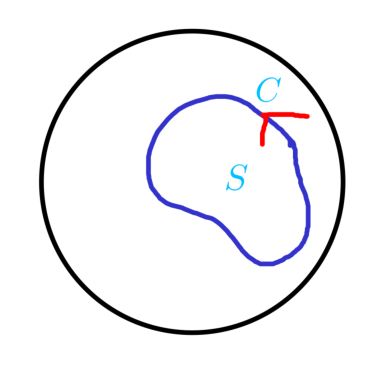
\includegraphics[width=0.4\linewidth]{berry-curv-as-magnetic}
	\caption{The geometric phase is the area integral of Berry curvature in the space of parameters, and also the line integral of Berry connection in the parameter space.}
	\label{fig:berry-curv-as-magnetic}
\end{figure}
Now, we can apply Stokes' theorem (in the manifold of the parameter space), and use the fact that the Berry curvature is the curl of the Berry connection, $\gamma = \int_S \vec{\Omega} \cdot d \vec{a}$.

This is analogous to the relation that the magnetic flux enclosed by a loop is the area integral of the magnetic field, $\Phi = \int \vec{B} \cdot d\vec{a}$.

The Berry phase can be regarded as the flux of the Berry curvature. Just like the magnetic field, the Berry curvature is gauge invariant \cite{BerryQuantalPhase1984}, it does not depend on the choice of the global phases of the eigenstate. Moreover, being the curl of a quantity (the Berry connection) the Berry curvature is divergenceless, $\nabla_{_{\vec{\lambda}}} \cdot \vec{\Omega} = 0$, just as the magnetic field, $\nabla_{_{\vec{r}}} \cdot \vec{B} = 0$. The similarity does not end here. We would soon see that the Berry curvature in the reciprocal space acts just like a magnetic field in reciprocal space, and it can give rise to Anomalous Hall response in absence of a (real space) magnetic field.

Although magnetic monopoles have not been found, the Berry curvature can often have a net non-zero flux through a closed surface in the parameter space, as if, it is due to a monopole in the parameter space \cite{tong2016lectures}. In reciprocal space, a Dirac cone with a mass can act like such a monopole.


\subsection{Geometric phase of electrons in a lattice}
Now, let us consider an electron in a periodic potential $V(\vec{r})$ (e.g. the potential due to a lattice, without any external electromagnetic fields). Its Hamiltonian is given by $\hat{H} = \frac{{\hat{\vec{p}}}^2}{2 m} + V(\hat{\vec{r}})$.

The eigenfunctions of this Hamiltonian are of the form,
$$\psi_{n, \vec{k}} (\vec{r}) = e^{i \vec{k}\cdot \vec{r}} u_{n,\vec{k}} (\vec{r})$$

Here $u_{n,\vec{k}} (\vec{r})$ is a function with the same periodicity as $V(\vec{r})$ (e.g. in a lattice, it would be periodic in every unit cell). The quantity $\hbar \vec{k}$ is known as the crystal momentum and $n$ is the band index. This result is known as \textit{Bloch's theorem} (See chapter 8 of \cite{book:AshcroftMermin76}). The crystal momentum is a good quantum number for an electron in a lattice, and it is conserved up to a reciprocal lattice vector (times $\hbar$).
Now, we can rewrite the eigenvalue equation $\left[-\frac{\hbar^2}{2m}\nabla^2 + V(\vec{r}) \right] \psi_{n, \vec{k}}(\vec{r}) = \varepsilon_{n,\vec{k}} \psi_{n, \vec{k}}(\vec{r})$ as,
\begin{equation}~\label{Eq:effectiveBlochEquation}
	\left[\frac{\hbar^2}{2m}(\vec{k} - i \nabla)^2 + V(\vec{r}) \right]u_{n,\vec{k}} (\vec{r}) = \varepsilon_{n,\vec{k}} u_{n,\vec{k}} (\vec{r})
\end{equation}

In this equation, $\vec{k}$ is just a parameter in the effective Hamiltonian. When we apply an external electromagnetic field, the crystal momentum is not anymore a good quantum number. Its evolution is governed by the Lorenz force, (See \cite{ralph2020berry} for derivation)

\begin{equation} \label{Eq:evolution-of-k}
	\boxed{\hbar \dot{\vec{k}} = -e\left(\vec{E} + \langle\dot{\vec{r}}\rangle \times \vec{B} \right)}
\end{equation}

As $\vec{k}$ (now a parameter of the effective Hamiltonian in Eq. \eqref{Eq:effectiveBlochEquation}) changes, it would give rise to a geometric phase, just like Eq. \eqref{Eq:BerryPhaseOriginal}. After a small time interval $\Delta t$, $\vec{k}$ would evolve to $\vec{k} + \dot{\vec{k}} \Delta t$ (we write $\dot{\vec{k}} \Delta t = \Delta \vec{k} $), and the periodic part of the Bloch wavefunction labeled with $\vec{k}$ would evolve as 
\begin{equation}\label{Eq:u-n-k-time-evolution}
	u_{n, \vec{k}} \rightarrow e^{i \gamma_{_{\vec{k}}}(\Delta t)} e^{-i \frac{\varepsilon_{_{\vec{k}}} \Delta t}{\hbar}} u_{n, \vec{k}+\Delta \vec{k}},
\end{equation} where $\gamma_{_{\vec{k}}}(\Delta t) =\vec{A}(\vec{k}) \cdot \Delta \vec{k}$, and $ \vec{A}(\vec{k})=i \bra{u_{n,\vec{k}}}\nabla_{_{\vec{k}}} \ket{u_{n,\vec{k}}}$ is the Berry connection \footnote{ $\bra{u_{n,\vec{k}}}\nabla_{_{\vec{k}}} \ket{u_{n,\vec{k}}}$ stands for $\int_\text{unit cell} d\vec{r} u^*_{n,\vec{k}} (\vec{r}) \nabla_{_{\vec{k}}} u_{n,\vec{k}}(\vec{r})$, where the normalization of $u_{n,\vec{k}}(\vec{r})$ is chosen such that $\int_\text{unit cell} d\vec{r} |u_{n,\vec{k}} (\vec{r})|^2 = 1$.} in the reciprocal space. Again, for a state labeled with a single $\vec{k}$, this geometric phase is an overall global phase, which would not show up in physical observables. However, if we take a linear superposition of Bloch wavefunctions with different values of $\vec{k}$, each of them would evolve with a different geometric phase $\gamma_n (\vec{k}) = \int_{0}^{t} dt' \vec{A(\vec{k})} \cdot \frac{d \vec{k}}{dt'} $, and we would soon see that the interference of such phase factors would lead to many interesting effects.

After all, this geometric phase is an effect of the Hamiltonian not commuting with itself at different times, for different values of the parameter $\vec{k}$. It can be easily verified that the commutator of the effective Hamiltonian with itself, for two different values of $\vec{k}$, namely, $\vec{k}_1$ and $\vec{k}_2$,
$$
\left[\frac{\hbar^2}{2m}(\vec{k}_1 - i \nabla)^2 + V(\vec{r}), \frac{\hbar^2}{2m}(\vec{k}_2 - i \nabla)^2 + V(\vec{r}) \right] = -\frac{i \hbar^2}{m} (\vec{k}_1 - \vec{k}_2)\cdot\nabla V(\vec{r})
$$

\section{Effects of Berry Curvature}
\subsection{Modification of semiclassical equations of motion of a wavepacket}\label{sec:Modification-semiclassical}
The probability density of the wavefunction $\psi_{n, \vec{k}} (\vec{r}) = e^{i \vec{k}\cdot \vec{r}} u_{n,\vec{k}} (\vec{r})$ is not localized anywhere, it is periodic over all unit cells (the blue curve in Fig. \ref{fig:wavepacket-and-bloch-wave}). We can construct a wave packet by forming a linear superposition of many such states, such that the wavepacket is localized at some point $\vec{r}_0$ in the real space (the red curve in Fig. \ref{fig:wavepacket-and-bloch-wave}), and its crystal momentum is also localized around a value of $\hbar \vec{k}_0$.

Although this wavepacket is localized in both real space and (crystal) momentum space, it does not violate Heisenberg's uncertainty relation, because for this wave packet, the product of the uncertainties in position and (crystal) momentum, $\Delta \vec{r} \Delta \vec{k}$ is still greater than $\frac{1}{2}$. While the wavepacket is spread over many unit cells, its spatial variation $\Delta \vec{r}$ is much smaller than the dimensions of the system, and $\Delta \vec{k}$ is much smaller than the dimensions of the Brillouin zone. As a result, in laboratory scale, the wavepacket behaves like a classical particle, with an almost localized value of position and crystal momentum.

\begin{figure}[h!]
	\centering
	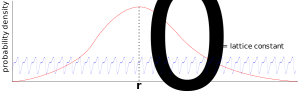
\includegraphics[width=0.7\linewidth]{wavepacket-and-Bloch-wave}
	\caption{The blue curve shows the probability density of a Bloch wavefunction. It is periodic over unit cells. The red curve shows a wavepacket which is localized in real space (although it is spread over many unit cells, it is localized compared to the dimensions of the system), as well as in crystal momentum space.}
	\label{fig:wavepacket-and-bloch-wave}
\end{figure}

It can be shown \cite{ralph2020berry} that for such a wavepacket, the expectation value of the position of its center evolves as \footnote{Note that this is the (group) velocity of the wavepacket. A single Bloch eigenstate does not have a definite velocity, because its density is periodic over every unit cell -- it does not have an well defined position, which could move with a certain velocity.},
\begin{equation}\label{Eq:evolution-of-r}
	\boxed{\langle\dot{\vec{r}}\rangle = \frac{1}{\hbar} \nabla{_{_{\vec{k}}}} \varepsilon_{_{\vec{k}}} - \langle\dot{\vec{k}}\rangle \times \vec{\Omega(\vec{k})}}
\end{equation}
Here, $\vec{\Omega(\vec{k})} = \nabla_{_{\vec{k}}} \times \vec{A(\vec{k})} = i \bra{\nabla_{_{\vec{k}}} u_{n,\vec{k}}}\times \ket{\nabla_{_{\vec{k}}} u_{n,\vec{k}}}$ is the Berry curvature in the reciprocal space. Also, here the energy eigenvalues are modified due to orbital magnetic moment $\vec{m}_{_{\vec{k}}}$ of an wavepacket (more about it in Section \ref{sec:OrbMagMom}) , $\varepsilon_{_{\vec{k}}} = \varepsilon_0(\vec{k}) - \vec{m}_{_{\vec{k}}} \cdot \vec{B}$, where $\varepsilon_0(\vec{k})$ is the original bandstructure energy at zero magnetic field.

In popular Solid State Physics textbooks, the second term in the RHS of Eq. \eqref{Eq:evolution-of-r}, involving the Berry curvature is omitted (e.g. see Eq. 8.51 of \cite{book:AshcroftMermin76}). This is most likely because people thought that the overall phase factor is unimportant. Also, we would soon see that the Berry curvature is identically zero unless certain symmetries are broken, and this is why its effects cannot be experimentally observed in most systems. 

This new term $- \langle\dot{\vec{k}}\rangle \times \vec{\Omega(\vec{k})}$ is known as the \textit{anomalous velocity}. To see why this term appears, let us first investigate how we can produce such a wavepacket, which is localized in both position space and crystal momentum space. This discussion is based on Section I. of \cite{ralph2020berry}. To make the wavepacket localized near $\vec{k}_0$ in the reciprocal space, consider a \textit{real} weight function $w(\vec{k} - \vec{k}_0)$, which is sharply localized about $\vec{k} = \vec{k}_0$. Now consider a linear superposition of the Bloch wavefunctions, of the form, $\int d\vec{k} w(\vec{k} - \vec{k}_0) e^{-i \vec{k} \cdot \vec{r}_0 } \left(e^{i \vec{k} \cdot\vec{r}} u_{n,\vec{k}}(\vec{r})\right)$. The expectation value of $\vec{k}$ of this wavefunction should be localized about $\vec{k}_0$. Then, near $\vec{r} = \vec{r}_0$, the functions $e^{i \vec{k} \cdot (\vec{r} -\vec{r}_0 )}$ constructively interfere, and we would expect the wavepacket to have a high probability density at $\vec{r}_0$. However, the functions $u_{n,\vec{k}}(\vec{r})$ may have different phases for different values of $\vec{k}$ at the same $\vec{r} = \vec{r}_0$, and then the waves would not constructively interfere.
After properly taking account of this (See Appendix \ref{app:calculation-of-<r>}), the wavefunction that is localized around $\expval{\vec{r}} = \vec{r}_0$, and peaked at crystal momentum $\hbar \vec{k}_0$ is found to be,
\begin{equation}\label{Eq:wavefunction-wavepacket}
	\psi(\vec{r}, t=0) = \int d\vec{k} w(\vec{k} - \vec{k}_0) e^{i \vec{A}(\vec{k_0})\cdot (\vec{k} - \vec{k}_0)} e^{-i \vec{k} \cdot \vec{r}_0 } \left(e^{i \vec{k} \cdot\vec{r}} u_{n,\vec{k}}(\vec{r})\right).
\end{equation}
Here $\vec{A}$ is again the Berry connection. After a small time $\Delta t$, the individual Bloch wavefunctions would then evolve as in Eq. \eqref{Eq:u-n-k-time-evolution}, and the wavefunction of the wavepacket would be,
$$\psi(\vec{r}, t=\Delta t) = \int d\vec{k} w(\vec{k} - \vec{k}_0) e^{i \vec{A}(\vec{k_0})\cdot (\vec{k} - \vec{k}_0)} e^{-i \vec{k} \cdot \vec{r}_0 } \left(e^{i (\vec{k} + \Delta\vec{k})\cdot\vec{r}} e^{i \vec{A}\cdot \vec{\Delta{k}}} e^{-i \frac{\varepsilon_{_{\vec{k}}} \Delta t}{\hbar}} u_{n, \vec{k}+\Delta \vec{k}} \right).$$
It can be shown (See Appendix. \ref{app:center-at-new-time}), that for this state, the expectation value of position is located at
$$\langle \vec{r} \rangle = \vec{r}_0 +  \frac{\Delta t}{\hbar} \nabla{_{_{\vec{k}}}} \varepsilon_{_{\vec{k}}}|_{_{\vec{k} = \vec{k}_0}} - \Delta \vec{k}_0 \times \vec{\Omega(\vec{k}_0)}.$$
The change in the expectation value of position after time $\Delta t$ is then, $\frac{\Delta t}{\hbar} \nabla{_{_{\vec{k}}}} \varepsilon_{_{\vec{k}}}|_{_{\vec{k} = \vec{k}_0}} - \Delta \vec{k}_0 \times \vec{\Omega(\vec{k}_0)}$. After dividing the change in position in $\langle{\vec{r}}\rangle$ by $\Delta t$, the expression of velocity in Eq. \eqref{Eq:evolution-of-r} follows.
\subsection{Violation of Liouville's theorem and Modification of phase space density}
We now drop the notation $\expval{\cdot}$ of expectation values, and denote $\expval{\vec{r}} \equiv \vec{r}$ and $\expval{\vec{k}} \equiv \vec{k}$ for a wavepacket localized at $\vec{r}$ and $\vec{k}$. Consider a point $\left(\vec{r},\vec{k}\right)$ in the phase space, with a small volume element $\Delta V_0$ around it. The points inside the volume element $\Delta V_0$ evolve as governed by the semiclassical equations of motion,
\begin{equation}\label{Eq:evolution-of-R}
	\boxed{\dot{\vec{r}} = \frac{1}{\hbar} \nabla{_{_{\vec{k}}}} \varepsilon_{_{\vec{k}}} - \dot{\vec{k}} \times \vec{\Omega(\vec{k})}}
\end{equation}

\begin{equation}\label{Eq:evolution-of-K}
	\boxed{\hbar \dot{\vec{k}} = -e\left(\vec{E} + \dot{\vec{r}} \times \vec{B} \right)}
\end{equation}
and suppose, they occupy a new volume $\Delta V(t)$ around the point $\left(\vec{r'},\vec{k'}\right)$ after time $t$. Then, the quantity $$\Delta V(t) \left(1 + \frac{e}{\hbar} \vec{B}\left(\vec{r}(t)\right) \cdot  \vec{\Omega}\left(\vec{k}(t)\right)\right)$$ remains a constant of motion \cite{BerryCorrectionPhaseSpaceNiu2005}(See Appendix \ref{app:phase-space-volume-evolution} for proof).

Liouville's theorem states that the volume $\Delta V$ occupied by a fixed number of points in the phase space remains invariant as the point $\left(\vec{r},\vec{k}\right)$ flows following the equations of motion (which are obtained from a classical Hamiltonian). In other words, the phase space density remains invariant. Here, that does not hold anymore (unless either of $\vec{B}$ or $\vec{\Omega}$ is zero, or they are orthogonal so that their dot product is zero). Note that the quantity defined above is a function of the local coordinates ($\vec{r}(t), \vec{k}(t)$), and does not depend on the trajectory.

Since the number of phase space points in the volume element $\Delta \vec{k} \Delta \vec{r} \left(1 + \frac{e}{\hbar} \vec{B}\left(\vec{r}(t)\right) \vec{\Omega}\left(\vec{k}(t)\right)\right)$ remains constant in time, if the magnetic field was initially zero, and we gradually turn on a homogeneous magnetic field, the number of states in the volume $\Delta \vec{k} \Delta \vec{r} \left(1 + \frac{e}{\hbar} \vec{B}(t) \cdot \vec{\Omega}\left(\vec{k}\right)\right)$ would be equal to the number of states in the initial volume $\Delta \vec{k} \Delta \vec{r}$.

As a result, when we calculate the expectation value of any operator $\mathcal{O}$ over all states, we would have to introduce an additional factor of $\left(1 + \frac{e}{\hbar} \vec{B} \cdot \vec{\Omega}\left(\vec{k}\right)\right)$ in the integrand, to correctly take account of all the states.
\begin{equation}~\label{Eq:operator-expval}
\expval{\mathcal{O}} = \int \frac{d\vec{k}}{(2\pi)^d} \left(1 + \frac{e}{\hbar} \vec{B} \cdot  \vec{\Omega}\left(\vec{k}\right)\right) \expval{\mathcal{O}}_{_{\vec{k}}} \tilde{g}_{\vec{k}}
\end{equation}
Here $\tilde{g}_{\vec{k}}$ is known as the distribution function, and counts the occupation number of electrons in a state labeled with $\vec{k}$. When no external fields are applied, in thermodynamic equilibrium, it is the Fermi distribution function, $\tilde{g}_{_{\vec{k}}} = f_{_{\vec{k}}} = \frac{1}{e^{\beta \left(\varepsilon_{_{\vec{k}}} - \mu \right)} + 1}$. When an electromagnetic field is applied, this equilibrium is disturbed, and we write the distribution function as $\tilde{g}_{_{\vec{k}}} = f_{_{\vec{k}}} + g_{_{\vec{k}}}$, where $g_{_{\vec{k}}}$ is the non-equilibrium part of the distribution (it is zero when there is no external electric field, or temperature gradient, or chemical potential gradient). We will see how to calculate it in Section \ref{sec:BTE-and-solution}.

Also, since Liouville's theorem does not hold anymore, we cannot obtain the equations of motion \eqref{Eq:evolution-of-R} and \eqref{Eq:evolution-of-K} from any (classical) effective Hamiltonian. 

\section{When do we get a non-zero Berry Curvature?}
\subsection{Spatial Inversion Symmetry}
Under spatial inversion symmetry, the polar vectors change sign, $\vec{r} \rightarrow -\vec{r}$, $\vec{k} \rightarrow -\vec{k}$, $\vec{E} \rightarrow -\vec{E}$, but axial vectors like $\vec{B} \rightarrow \vec{B}$ remain unchanged. Also, since $\vec{\Omega} = \nabla_{_{\vec{k}}} \times A$ itself is an axial vector, under spatial inversion it changes as, $\vec{\Omega(\vec{k})} \rightarrow \vec{\Omega(\vec{-k})}$.

Then, if we apply the spatial inversion operator, the LHS of Eq. \eqref{Eq:evolution-of-r} changes sign, and then the RHS must change sign too. Then, $\dot{\vec{k}}\times \vec{\Omega(\vec{k})}$ must also change overall sign. But, under spatial inversion,  $\dot{\vec{k}}\times \vec{\Omega(\vec{k})} \rightarrow (-\vec{\dot{k}})\times \vec{\Omega(\vec{-k})}$, and this must be equal to $-\dot{\vec{k}}\times \vec{\Omega(\vec{k})}$, and we must have, 
\begin{equation}\label{Eq:OmegaSpatialInversion}
	\vec{\Omega}(-\vec{k}) = \vec{\Omega}(\vec{k}),
\end{equation}
when spatial inversion symmetry is present.\\\\

\subsection{Time Reversal Symmetry}
Under time reversal, the quantities $\vec{\dot{r}} \rightarrow -\vec{\dot{r}}$, $\vec{k} \rightarrow -\vec{k}$ change sign, whereas $\vec{\dot{k}} \rightarrow \vec{\dot{k}}$ remains the same. The spin of the electron also flips, $\vec{\sigma} \rightarrow -\vec{\sigma}$.

If we apply the time reversal operator, the LHS of Eq. \eqref{Eq:evolution-of-r} changes sign, and then $\dot{\vec{k}}\times \vec{\Omega(\vec{k})}$ must change an overall sign too. In general, the Berry curvature depends on the band index and the spin, and it follows that when time reversal symmetry is present,
\begin{equation}\label{Eq:OmegaTimeReversal}
	\vec{\Omega}_{n,\sigma}(-\vec{k}) = -\vec{\Omega}_{n,-\sigma}(\vec{k}).
\end{equation}

When there is no spin orbit coupling, the spatial parts of the wavefunctions for up and down spins are the same, consequently the Berry curvatures are the same too (because the Berry Curvature $\vec{\Omega}(\vec{k}) = i \bra{\nabla_{_{\vec{k}}} u_{n,\vec{k}}}\times \ket{\nabla_{_{\vec{k}}} u_{n,\vec{k}}}$ is a function of the spatial part of the wavefunction).

Then, when the spin orbit coupling is negligible, under time reversal symmetry,
\begin{equation}\label{Eq:OmegaTimeReversalzeroSpinOrbit}
	\vec{\Omega}_{n,\sigma}(-\vec{k}) = -\vec{\Omega}_{n,\sigma}(\vec{k}).
\end{equation}
\textbf{Note}: Even when the time reversal symmetry is broken due to an external magnetic field, we continue to have the same Bloch wavefunctions (when the magnetic field is low enough), and since the Berry curvature is a function of the Bloch wavefunctions, in case there was time reversal symmetry before applying the magnetic field, the result (Eq. \eqref{Eq:OmegaTimeReversalzeroSpinOrbit}) continues to hold even after applying it (until the magnetic field is so high that the bandstructure is heavily modified, and we enter the regime of Landau levels).

\subsection{Conditions for non-Zero Berry Curvature}
As a result, when both spatial inversion and time reversal symmetry exist, and spin orbit coupling is negligible, then, combining Eq. \eqref{Eq:OmegaSpatialInversion} and Eq. \eqref{Eq:OmegaTimeReversalzeroSpinOrbit} $\vec{\Omega}_{n,\sigma}(-\vec{k}) = \vec{\Omega}_{n,\sigma}(\vec{k}) = -\vec{\Omega}_{n,\sigma}(\vec{k})$, i.e. $\vec{\Omega} \equiv 0$ for any $\vec{k}$.

Then, to get a non-zero Berry curvature \cite{ralph2020berry}, either time reversal or spatial inversion symmetry must be broken, or there must be significant spin orbit coupling. Note that these conditions are necessary to get a non-zero Berry curvature, but they may not be sufficient.

In any metal, time reversal symmetry is already present, and the spatial inversion symmetry is present in BCC, FCC and simple cubic lattices. As a result, the Berry curvature is identically zero in most metals. Now we understand why the effects (e.g see section \ref{sec:AHE}) of the additional term in Eq. \eqref{Eq:evolution-of-R} were not seen in early transport experiments, and were not described in elementary solid state physics textbooks.
 
A non-zero Berry curvature can present in biased Bilayer graphene \cite{PhysRevB.79.245424, PhysRevLett.99.236809}, and also in topological materials like Chern Insulator and Weyl semimetal. These materials were not experimentally realized before 21\textit{st} century.
 
\section{Decoupling of the equations of motion and their simplification}

The coupled differential equations of motion for $\dot{\vec{r}}$ and $\dot{\vec{k}}$ (Eq. \eqref{Eq:evolution-of-R} and Eq. \eqref{Eq:evolution-of-K}) can be easily decoupled with some vector algebra (See Appendix \ref{app:decoupling-of-eom}), and the resulting decoupled equations are,

\begin{equation}~\label{Eq:SC_EOM_r_dot}
	\dot{\vec{r}} = \frac{\frac{1}{\hbar} \frac{\partial \varepsilon}{\partial \vec{k}} + \frac{e}{\hbar} (\vec{E}\times\vec{\Omega}) + \frac{e}{\hbar^2} (\vec{\Omega} \cdot \frac{\partial \varepsilon}{\partial \vec{k}} )\vec{B}}{1 + \frac{e}{\hbar} \vec{B}\cdot\vec{\Omega}}
\end{equation}

\begin{equation}~\label{Eq:SC_EOM_k_dot}
	\dot{\vec{k}} = -\frac{\frac{e}{\hbar} \vec{E} +\frac{e}{\hbar^2} \frac{\partial \varepsilon}{\partial \vec{k}} \times \vec{B} + \frac{e^2}{\hbar^2} (\vec{E}\cdot\vec{B}) \vec{\Omega}}{1 + \frac{e}{\hbar} \vec{B}\cdot\vec{\Omega}}
\end{equation}
In a \textit{2D sample}, $\vec{\Omega}$ is along the $z$ axis, while $\frac{\partial \varepsilon}{\partial \vec{k}}$ is in the $xy$ plane, then $\vec{\Omega} \cdot \frac{\partial \varepsilon}{\partial \vec{k}} = 0$. Also, in \textit{2D}, $\vec{\Omega}$ is along the $z$ axis, whereas $\vec{k}$ is restricted to the $xy$ plane. Then we can neglect the term $(\vec{E}\cdot\vec{B}) \vec{\Omega}$ in the expression of $\dot{\vec{k}}$.
Then the equations \eqref{Eq:SC_EOM_r_dot} and \eqref{Eq:SC_EOM_k_dot} simplify to,
\begin{equation}~\label{Eq:SC_EOM_r_dot_decoupled}
	\boxed{\dot{\vec{r}} = \frac{\frac{1}{\hbar} \frac{\partial \varepsilon}{\partial \vec{k}} + \frac{e}{\hbar} (\vec{E}\times\vec{\Omega})}{1 + \frac{e}{\hbar} \vec{B}\cdot\vec{\Omega}}}
\end{equation}

\begin{equation}~\label{Eq:SC_EOM_k_dot_decoupled}
	\boxed{\dot{\vec{k}} = -\frac{\frac{e}{\hbar} \vec{E} +\frac{e}{\hbar^2} \frac{\partial \varepsilon}{\partial \vec{k}} \times \vec{B}}{1 + \frac{e}{\hbar} \vec{B}\cdot\vec{\Omega}}}
\end{equation}
\chapter{Strategy of Calculation of Thermal and Heat Currents}
To calculate the total electric current density, we need to sum the expectation value of the electric current operator \footnote{\textbf{Convention}: Charge of electron is $-e$ everywhere in the thesis.}, $\hat{\vec{j}_e} = -e \hat{\dot{\vec{r}}}$ over all states, and we substitute $\expval{\hat{\dot{\vec{r}}}}_{_{\vec{k}}}$ with its value in Eq. \eqref{Eq:SC_EOM_r_dot_decoupled}. Without the Berry curvature, the current density would be, $\expval{\hat{\vec{j}}_e} = \int \frac{d\vec{k}}{(2\pi)^d} (- e \dot{\vec{r}})_{_{\vec{k}}} ({f}_{\vec{k}} + {g}_{\vec{k}})$, but in presence of the Berry curvature, we need to take account of the phase space volume correction (see Eq. \eqref{Eq:operator-expval}), and the expression for the current density is,

\begin{equation} \label{Eq:electric-current}
	\expval{\hat{\vec{j}}_e} = \int \frac{d\vec{k}}{(2\pi)^d} \left(1 + \frac{e}{\hbar} \vec{B} \cdot  \vec{\Omega}\left(\vec{k}\right)\right) (- e \dot{\vec{r}})_{_{\vec{k}}} ({f}_{\vec{k}} + {g}_{\vec{k}})
\end{equation}

To calculate the heat current operator, consider a closed surface in a system, through which it can exchange energy in the form of heat, and also particles. From the first law of thermodynamics we know that the heat gained by the system inside this volume satisfies, $dQ = dE - \mu dN$, where $\mu$ is the chemical potential, $E$ is the energy of the system enclosed by the surface, and $N$ is the number of particles inside the surface. From this relation, it follows that $\vec{j}_Q = \vec{j}_E - \mu \vec{j}_N$, where $\vec{j}_Q$, $\vec{j}_E$, and $\vec{j}_N$ are the heat current density, energy current density, and number current density \footnote{the electric current density is just the electron charge times the number current density, $\vec{j}_e = -e \vec{j}_N$}, respectively. Now we promote the current densities to their respective operators, and obtain the relation,
\begin{equation} 
	\expval{\hat{\vec{j}}_Q}_{_{\vec{k}}} = \expval{\hat{\vec{j}}_E}_{_{\vec{k}}} - \mu \expval{\hat{\vec{j}}_N}_{_{\vec{k}}} = \varepsilon_{_{\vec{k}}} \expval{\dot{\vec{r}}}_{_{\vec{k}}} - \mu \expval{\dot{\vec{r}}}_{_{\vec{k}}}
\end{equation}

The total heat current is then given by,
\begin{equation} \label{Eq:heat-current}
	\expval{\hat{\vec{j}}_Q} = \int \frac{d\vec{k}}{(2\pi)^d} \left(1 + \frac{e}{\hbar} \vec{B} \cdot  \vec{\Omega}\left(\vec{k}\right)\right) (\varepsilon_{_{\vec{k}}} - \mu) \dot{\vec{r}}_{_{\vec{k}}} ({f}_{\vec{k}} + {g}_{\vec{k}})
\end{equation}

We can now put $d = 2$ and use the expression of $\dot{\vec{r}}$ in Eq. \eqref{Eq:SC_EOM_r_dot_decoupled} to further simplify Eq. \eqref{Eq:electric-current} and Eq. \eqref{Eq:heat-current}, and obtain \footnote{\textbf{This is not the complete story}. There are more terms because the electron is not completely localized in the center of the wavepacket, and there can be circulating magnetization current, which play an important role. More about that in section \ref{chap:OrbMag}.},
\begin{equation}~\label{Eq:electric-current-simplified}
	\expval{\hat{\vec{j}}_e} = -e \int \frac{d\vec{k}}{(2\pi)^2} ({f}_{\vec{k}} + {g}_{\vec{k}}) \left[\frac{1}{\hbar} \frac{\partial \varepsilon_{_{\vec{k}}}}{\partial \vec{k}} + \frac{e}{\hbar} (\vec{E}\times\vec{\Omega}(\vec{k}))\right]
\end{equation}

\begin{equation} \label{Eq:heat-current-simplified}
	\expval{\hat{\vec{j}}_Q} = \int \frac{d\vec{k}}{(2\pi)^2} (\varepsilon_{_{\vec{k}}} - \mu) ({f}_{\vec{k}} + {g}_{\vec{k}}) \left[\frac{1}{\hbar} \frac{\partial \varepsilon_{_{\vec{k}}}}{\partial \vec{k}} + \frac{e}{\hbar} (\vec{E}\times\vec{\Omega}(\vec{k}))\right]
\end{equation}

\section{An analysis of contribution of different terms in the above integrals}
\subsection{The contribution from the equilibrium part of the distribution, and the band structure part of the velocity is \textbf{zero}}~\label{sec:zeroCont}
$\varepsilon_0 (\vec{k})$ is usually an even function of $\vec{k}$, when the system has time reversal symmetry. Then the Fermi distribution $f_{_{\vec{k}}} = \frac{1}{1+ e^{\beta\left(\varepsilon_0 (\vec{k}) - \mu\right)}}$ is also an even function, and the band structure part of the velocity, $\frac{\partial \varepsilon_0 (\vec{k})}{\partial \vec{k}}$ is an odd function of $\vec{k}$. Then, the integrals $\int d\vec{k} f_{_{\vec{k}}} \frac{\partial \varepsilon_0 (\vec{k})}{\partial \vec{k}}$ and $\int d\vec{k} f_{_{\vec{k}}} \left(\varepsilon_0 (\vec{k}) - \mu\right) \frac{\partial \varepsilon_0 (\vec{k})}{\partial \vec{k}}$ in the expressions of the electric and heat currents are zero, because the overall integrand is an odd function.

When there is a magnetic field, we get a modified energy $\varepsilon_{_{\vec{k}}} = \varepsilon_0 (\vec{k}) - \vec{m}_{\vec{k}} \cdot \vec{B}$, and this simple argument does not hold anymore. We would still expect the net transport current to be zero, when there is no external electric field or chemical potential gradient or temperature gradient, but there is a non-zero magnetic field.
Then, the modified Fermi distribution function would be,
$f_{\vec{k}} = f(\varepsilon_0(\vec{k})) - \vec{m}\cdot\vec{B}) = f(\varepsilon_0(\vec{k}) + \sum_{n=1}^{\infty} (-1)^n \frac{\partial^n f}{\partial {\varepsilon_0}^n} \frac{(\vec{m}\cdot \vec{B})^n}{n!}$.

Then, the relevant term in the electric current density would be,
$$
\int \frac{d\vec{k}}{(2\pi)^d} \left[f(\varepsilon_0(\vec{k})) + \sum_{n=1}^{\infty} (-1)^n \frac{\partial^n f}{\partial {\varepsilon_0}^n} \frac{(\vec{m}\cdot \vec{B})^n}{n!}\right] \left[\frac{\partial \varepsilon_0 (\vec{k})}{\partial \vec{k}} - \frac{\partial }{\partial \vec{k}}(\vec{m}\cdot\vec{B}) \right]
$$

The zeroeth order term in magnetic field is 0, as $\int \frac{d\vec{k}}{(2\pi)^d} f(\varepsilon_0(\vec{k})) \frac{\partial \varepsilon_0} {\partial \vec{k}} = 0$, as the overall integrand is an odd function of $\vec{k}$, as explained in the previous paragraph.
	
Consider the term $n$-th order in the magnetic field,

$$
\begin{aligned}
	& \int_{\text{BZ}} \frac{d\vec{k}}{(2\pi)^d} (-1)^{n} \frac{\partial^{n} f}{\partial \varepsilon_{0}^{n}} \frac{(\vec{m} \cdot \vec{B})^n}{n !}\frac{\partial \varepsilon_0 (\vec{k})}{\partial \vec{k}} - (-1)^{(n-1)}  \frac{\partial^{n-1} f}{\partial \varepsilon_{0}^{n-1}} \frac{(\vec{m} \cdot \vec{B})^{n-1}}{(n-1) !} \frac{\partial }{\partial \vec{k}}(\vec{m}\cdot\vec{B}) \\
	= & (-1)^n \int_{\text{BZ}} \frac{d\vec{k}}{(2\pi)^d} \left(\frac{\partial}{\partial \vec{k}}\frac{\partial^{n-1} f}{\partial \varepsilon_{0}^n}\right) \frac{(\vec{m} \cdot \vec{B})^n}{n !} + \frac{\partial^{n-1} f}{\partial \varepsilon_{0}^{n-1}} \frac{(\vec{m} \cdot \vec{B})^{n-1}}{(n-1) !} \frac{\partial }{\partial \vec{k}}(\vec{m}\cdot\vec{B}) \\
	= & (-1)^n \int_{\text{BZ}} \frac{d\vec{k}}{(2\pi)^d} \frac{\partial}{\partial \vec{k}} \left[\frac{\partial^{n-1} f}{\partial \varepsilon_{0}^n} \frac{(\vec{m} \cdot \vec{B})^n}{n !}\right] = 0 ,
\end{aligned}
$$
because the integral of the gradient of a periodic scalar, over the Brillouin Zone is zero (see Appendix I of \cite{book:AshcroftMermin76} for proof).
Similarly, it can be shown that the similar term for energy current is zero up to all orders in magnetic field.

These results are expected because there should not be any transport currents in equilibrium (in absence of electric field, chemical potential gradient or temperature gradient).
\subsection{Terms contributing to quadratic order  in external fields (we neglect them)}~\label{sec:quadCont}
In Eq. \eqref{Eq:gnonzeroE} and Eq. \eqref{Eq:g_non_zero_chem_temp_grad} it has been shown that up to leading order, the non-equilibrium part of the distribution function, ${g}_{\vec{k}}$ is a linear function of the electromagnetic field and the gradients of chemical potential and temperature. Then, the term ${g}_{\vec{k}} (\vec{E}\times\vec{\Omega}(\vec{k}))$ is a quadratic function of the externally applied fields, and we neglect its contribution in the expressions of electric and heat current densities.
\subsection{Terms contributing to linear order in external fields}~\label{sec:linearCont}
The rest of the terms ($ {f}_{\vec{k}} (\vec{E}\times\vec{\Omega}) $ and ${g}_{\vec{k}} \frac{\partial \varepsilon_{_{\vec{k}}}}{\partial \vec{k}}$) are linear in the external electric field, and chemical potential gradient, and temperature gradient, and henceforth, we would only consider these terms.
\section{An illustration of the above procedure: the Anomalous Hall effect and quantized off-diagonal electric conductivity}~\label{sec:AHE}
When there is a non-zero Berry curvature, a sample can show a Hall response even in absence of a magnetic field, and more astonishingly, the Hall conductance is quantized. This is known as the anomalous Hall effect.

Suppose we apply an electric field along $x$ direction on a 2D sample, and the magnetic field $\vec{B} = 0$. There are no temperature gradient or chemical potential gradient.

It can be shown that  $g_{\vec{k}} = \frac{\partial f} {\partial \varepsilon}
\frac{\tau}{\hbar} \frac{\partial \varepsilon}{\partial \vec{k}}\cdot e \vec{E}$, up to linear order in $\vec{E}$ (this is a special case of Eq. \eqref{Eq:gnonzeroE}, with $\vec{B} = 0$). Ignoring the terms with quadratic and zero contribution, (See section \ref{sec:quadCont} and \ref{sec:zeroCont}), the electric current $\expval{\hat{\vec{j}}_e} = -e \int \frac{d\vec{k}}{(2\pi)^2} \left[{f}_{\vec{k}} \frac{e}{\hbar} (\vec{E}\times\vec{\Omega(\vec{k})}) + {g}_{\vec{k}} \frac{1}{\hbar} \frac{\partial \varepsilon}{\partial \vec{k}}\right] $. The second term contributes to $\sigma_{xx}$, and it is nothing but a regular Ohmic response (analyzed in section \ref{subsubsec:regularOhmic}). The first term \footnote{It is to be noted that this is due to the intrinsic Fermi distribution function, and is independent of scattering (which is responsible for the non-equilibrium part of the distribution function, ${g}_{\vec{k}}$).} leads to a current perpendicular to the applied electric field,
$$\expval{\hat{\vec{j}}_e}_y = \frac{e^2}{2 \pi \hbar} \vec{E}_x \int \frac{d\vec{k}}{2\pi} {f}_{\vec{k}} \vec{\Omega}(\vec{k}) = \frac{e^2}{2 \pi \hbar} \vec{E}_x \int_{\text{filled}} \frac{d\vec{k}}{2\pi} \vec{\Omega}(\vec{k}).$$
For a fully filled band, the integral of $\frac{1}{2\pi}\Omega(\vec{k})$ over the first Brillouin zone is an integer, and it is called the first Chern Number (see \ref{sebsec:integer-chern-argument}), which we denote as $\mathcal{C}$. Then, the off-diagonal part of the conductivity tensor is \textit{quantized}\footnote{The factor of $(1 + \frac{e}{\hbar} \vec{B}\cdot\vec{\Omega})$ gets canceled in the numerator (from the phase space connection) and the denominator (from the expression of $\dot{\vec{r}}_{_{\vec{k}}}$), as seen in Eq. \eqref{Eq:electric-current-simplified} and Eq. \eqref{Eq:heat-current-simplified}, and the fact that the ``Anomalous Hall response is quantized'' holds true even when there is a non-zero magnetic field.},
$$\sigma_{xy} = \frac{\vec{j}_y}{\vec{E}_x} = \frac{e^2}{2\pi \hbar} \mathcal{C}.$$
Here we have a current along $y$ axis, while the external electric field is along the $x$ axis. This is like the Hall effect, but \textit{without} a magnetic field, hence it is called the \textit{Anomalous} Hall effect.
It can be similarly shown that
$$\sigma_{yx} = - \frac{e^2}{2\pi \hbar} \mathcal{C} = -\sigma_{xy}.$$

Note that this is \textit{not} the Quantum Hall Effect, where the diagonal conductivity $\sigma_{xx}$ also becomes quantized under very high magnetic fields, and the bandstructures are replaced by Landau levels. In this paper we are working in the low magnetic field regime, and in this particular context of anomalous Hall effect, the magnetic field is zero.
 
\subsection{When do we get non-zero Anomalous Hall response?}
When time reversal symmetry is present, the Berry curvature is an odd function, $\vec{\Omega}(\vec{k}) = - \vec{\Omega}(\vec{-k})$, and its integral over the Brillouin zone is zero (consequently, the Chern number is zero).
Therefore, we need a \textit{broken time reversal symmetry} to get Anomalous Hall Effect.


\section{Einstein and Onsager relations}~\label{sec:Einstein-Onsager}
In linear regime of thermoelectric transport, we 
can express the electric and thermal currents as,

\begin{equation}~\label{Eq:TrasportCoeffs}
	\begin{aligned}
		\expval{\hat{\vec{j}}_e} &= \stackrel{\leftrightarrow}{L}_{11} \cdot \left(\vec{E} + \nabla \frac{\mu}{e}\right) + \stackrel{\leftrightarrow}{L}_{12} \cdot (-\nabla{T})  \\
		\expval{\hat{\vec{j}}_Q} &= \stackrel{\leftrightarrow}{L}_{21} \cdot \left(\vec{E} + \nabla \frac{\mu}{e}\right)  + \stackrel{\leftrightarrow}{L}_{22} \cdot (-\nabla{T}) 
	\end{aligned}
\end{equation}
Here $\stackrel{\leftrightarrow}{L}_{i j}$ ($i,j \in {1,2}$) are tensors, they act on a vector to give a vector. $\stackrel{\leftrightarrow}{L}_{1 1}$ is the electric conductivity, $\stackrel{\leftrightarrow}{L}_{2 2}$ is the thermal conductivity\footnote{Here we denoted thermal conductivity as the heat current per unit temperature gradient, at zero electric field or zero chemical potential gradient. Sometimes, thermal conductivity is denoted as heat current per unit temperature gradient, when the net electric current is zero (an internal electrochemical potential gradient is generated to maintain zero electric current, but that internal electrochemical potential gradient in turn contributes to the heat current). In that case, it can be shown that (see Eq. 13.56 of \cite{book:AshcroftMermin76}) the heat current (i.e. the heat conductivity, because we set $\nabla T = 1$) is $\stackrel{\leftrightarrow}{L}_{22} - \stackrel{\leftrightarrow}{L}_{21} (\stackrel{\leftrightarrow}{L}_{11})^{-1} \stackrel{\leftrightarrow}{L}_{12}$. But this additional term is a small correction, it is of the order $\left(\frac{k_B T}{\varepsilon_F}\right)^2$.}, and $\stackrel{\leftrightarrow}{L}_{1 2}$, $\stackrel{\leftrightarrow}{L}_{2 1}$ are related to the Seebeck and Peltier coefficients.

The symmetry between $\vec{E} \longleftrightarrow \frac{1}{e}\nabla \mu$ is known as the \textit{Einstein relation}. Physically speaking, the thermoelectric response for an electric field and an equivalent chemical potential gradient would be identical.
 
Experimentally, it is found that
\begin{equation}\label{Eq:Onsager-relation}
	\stackrel{\leftrightarrow}{L}_{21} = T \stackrel{\leftrightarrow}{L}_{12}.
\end{equation}
Relations like this are known as \textit{Onsager reciprocal relation}s \cite{OnsagerPhysRev.37.405}. In this particular case, the Onsager relation is equivalent to the relation between the Seebeck and Peltier coefficients (See chapter \ref{chap:Seebeck-Peltier-Nernst}).

These quantities are often expressed \cite{Ussishkin_2002} in the alternative notation $\stackrel{\leftrightarrow}{L}_{1 1} = \stackrel{\leftrightarrow}{\sigma}$, $\stackrel{\leftrightarrow}{L}_{1 2} = \stackrel{\leftrightarrow}{\alpha}$, $\stackrel{\leftrightarrow}{L}_{2 1} = \stackrel{\leftrightarrow}{\tilde{\alpha}}$, $\stackrel{\leftrightarrow}{L}_{2 2} = \stackrel{\leftrightarrow}{\kappa}$.

\subsection{(Apparent) Violation of Einstein and Onsager Relations in presence of Berry Curvature}\label{sec:Einstein-Onsager-violation}
While the microscopic theoretical validations of the Einstein and the Onsager relations have been established (see chapter 7 of \cite{book:ZimanSolidState} and chapter 13 of \cite{book:AshcroftMermin76}), they are tricky to establish when a Berry curvature is present.

For an example, consider the Anomalous Hall effect. It happens due to the equilibrium part of the electronic distribution (the Fermi distribution function), and the Berry curvature part ($\vec{E} \times \vec{\Omega})$ of the velocity of the electron wavepacket. However, there are no terms like $\nabla \mu \times \vec{\Omega}$ or $\nabla T \times \vec{\Omega}$. As a result, apparently, there are no off-diagonal thermoelectric response when $\vec{E} = 0$ (but $\nabla \mu \neq 0$ or $\nabla T \neq 0$), and both Einstein and Onsager relations are violated.

\textbf{Resolution}: In presence of the Berry curvature, the Bloch wavepacket can have a orbital magnetic moment (see Chapter \ref{chap:OrbMag}), i.e., the electron density is circulating about its center of mass (more specifically, the local value of the momentum, $\psi^*(\vec{r}) (-i \hbar \nabla_{\vec{r}}) \psi(\vec{r})$ circulates about the center $\vec{r}_0$). This circulating current is known as the magnetization current, $\vec{j}_M = \nabla \times \vec{M}$, which cannot be measured in transport experiments. The current measured in transport experiments is the transport current, which is obtained by subtracting the magnetization current from the total current, $\vec{j}_{\text{tr}} = \vec{j} - \vec{j}_M$. It can be theoretically shown that the Onsager and the Einstein relations are valid for the transport electric current and the transport heat current.

In the next chapter, we show that the Einstein and the Onsager relations remain valid for current densities arising from the non-equilibrium part of the distribution, after which we would get back to resolving the issue of violation of the Einstein and Onsager relations for Anomalous Hall terms.

\chapter{Boltzmann Transport Equation and its solution}\label{sec:BTE-and-solution}
A Bloch wavefunction is an eigenstate of the periodic potential of a perfect lattice, as if, an electron in a Bloch wavefunction can move throughout the system without getting scattered by the ions. However, in a real system, there are lattice defects, lattice vibrations (phonons) and impurities, all of which scatter the electron to a different state. In equilibrium, the electron distribution function reduces to the Fermi distribution, $f_{_{\vec{k}}} = \frac{1}{e^{\beta \left(\varepsilon_{_{\vec{k}}} - \mu \right)} + 1}$. When an external electromagnetic field, or a chemical potential gradient, or a thermal gradient is applied, the local distribution is modified due to scattering between different states. When the system is perturbed slightly out of equilibrium (i.e. when the external electromagnetic fields are much smaller than the atomic fields), the distribution is slightly modified from the Fermi distribution, $\tilde{g}_{_{\vec{k}}} = f_{_{\vec{k}}} + g_{_{\vec{k}}}$, where $|g_{_{\vec{k}}}| \ll f_{_{\vec{k}}}$. To calculate $g_{_{\vec{k}}}$, we employ the following idea. Consider an electron wavepacket in the phase space point $(\vec{r},\vec{k})$, and it evolves according to the equations of motion. Then, the rate of change of the distribution function is given by the convective derivative in the phase space, $\left[\frac{\partial}{\partial t} +  \dot{\vec{k}}\cdot\frac{\partial}{\partial \vec{k}} + \dot{\vec{r}}\cdot\frac{\partial}{\partial \vec{r}} \right]\tilde{g}_{_{\vec{k}}}$. The scattering processes would try to bring it back to the local equilibrium, and we expect it to be faster when the deviation from the equilibrium is more. Then, phenomenologically, we can write that the convective derivative is proportional to the deviation from equilibrium, with the proportional constant being the scattering timescale $\tau_{_{\vec{k}}}$, the timescale over which the distribution exponentially reaches a local equilibrium. This assumption is known as the relaxation time approximation, and under this approximation, the non-equilibrium part of the distribution function follows the Boltzmann Transport Equation (BTE), $\left[\frac{\partial}{\partial t} +  \dot{\vec{k}}\cdot\frac{\partial}{\partial \vec{k}} + \dot{\vec{r}}\cdot\frac{\partial}{\partial \vec{r}} \right]\tilde{g}_{_{\vec{k}}} = -\frac{g_{_{\vec{k}}}}{\tau}$. The scattering timescale can in general depend on $\vec{k}$. We would soon see that only the values of $\vec{k}$ on the Fermi surface would contribute a non-zero amount to the transport, and we assume that there is a constant scattering time $\tau$ on the Fermi surface. 

This formalism is based on Chapter 7 of \cite{book:ZimanSolidState}, where the author has calculated the electric and thermal conductance tensors in the absence of Berry curvature. Here, we extend the formalism for a non-zero Berry curvature. When the external fields are time independent, we can drop the explicit partial derivative with respect to time, and the Boltzmann Transport Equation can be cast into the form,
\begin{equation}~\label{Eq:BTE2}
	\frac{g}{\tau} + \dot{\vec{k}}\cdot\frac{\partial}{\partial \vec{k}} g + \dot{\vec{r}}\cdot\frac{\partial}{\partial \vec{r}} g = -\dot{\vec{k}}\cdot\frac{\partial}{\partial \vec{k}}f - \dot{\vec{r}}\cdot\frac{\partial}{\partial \vec{r}}f.
\end{equation}
Using the decoupled equations of motion, right hand side of Eq. \eqref{Eq:BTE2} simplifies to (see Appendix \ref{app:sec:BTE_simp_RHS}),
$$\frac{\partial f}{\partial \varepsilon}\frac{1}{1 + \frac{e}{\hbar} \vec{B}\cdot\vec{\Omega}}
\frac{1}{\hbar} \frac{\partial \varepsilon}{\partial \vec{k}}\cdot\left[e \vec{E} + \nabla{\mu} + \nabla T \frac{\varepsilon - \mu}{T}\right] .
$$
Here we see that we can exchange $\vec{E} \leftrightarrow \nabla \mu$, i.e., the Einstein relation holds. We would show that the Onsager relation holds as well.
We assume that the fields are constant in space, and drop the term containing $\frac{\partial{g}}{\partial \vec{r}}$.

\textbf{Validity of neglecting this term}: When we solve the equation after discarding this term, we would find that (See Eq. ~\eqref{Eq:gnonzeroE}) this term ($\dot{\vec{r}} \cdot 
 \frac{\partial{g}}{\partial \vec{r}}$) is second order in the applied fields. Then up to linear order, we can discard this term. Then, the BTE becomes,
\begin{equation}~\label{Eq:BTE_semiFinal_Form}
	\frac{g}{\tau} -\frac{\frac{e}{\hbar} \vec{E} + \frac{e}{\hbar^2} \frac{\partial \varepsilon}{\partial \vec{k}} \times \vec{B}}{1 + \frac{e}{\hbar} \vec{B} \cdot \vec{\Omega}} \cdot\frac{\partial}{\partial \vec{k}} g = \frac{\partial f}{\partial \varepsilon}\frac{1}{1 + \frac{e}{\hbar} \vec{B} \cdot \vec{\Omega}}
	\frac{1}{\hbar} \frac{\partial \varepsilon}{\partial \vec{k}}\cdot\left[e \vec{E} + \nabla{\mu} + \nabla T \frac{\varepsilon - \mu}{T}\right]
\end{equation}
We can further simplify this equation. If we neglect the term $\vec{E} \cdot \frac{\partial g}{\partial \vec{k}}$ in the LHS, we would find (in the next section) that $g$ is a linear function of the electric field, the chemical potential gradient, and the temperature gradient. Then, $\vec{E} \cdot \frac{\partial g}{\partial \vec{k}}$ would be quadratic in the applied fields, and the solution would remain self-consistent if we neglect it. In other words, if we first neglect it, find the solution, and treat this terms as a perturbation, it would turn out to be quadratic, and we would neglect it anyway. Finally, the equation we would have to solve is,
\begin{equation}~\label{Eq:BTE_Final_Form}
	\boxed{\frac{g}{\tau} -\underbrace{\frac{\frac{e}{\hbar^2} \frac{\partial \varepsilon}{\partial \vec{k}} \times \vec{B}}{1 + \frac{e}{\hbar} \vec{B} \cdot \vec{\Omega}} \cdot\frac{\partial}{\partial \vec{k}} g}_{\text{treated as a perturbation}} = \frac{\partial f}{\partial \varepsilon}\frac{1}{1 + \frac{e}{\hbar} \vec{B} \cdot \vec{\Omega}}
	\frac{1}{\hbar} \frac{\partial \varepsilon}{\partial \vec{k}}\cdot\left[e \vec{E} + \nabla{\mu} + \nabla T \frac{\varepsilon - \mu}{T}\right]}
\end{equation}
We treat the second term in the LHS as a perturbation. An order of the magnitude estimate in Appendix \ref{app:perturbation_validation} shows that the magnetic field needs to be of the order of hundreds of Tesla for this term to be of the same magnitude as the other term, $\frac{g}{\tau}$. Since the magnetic field in the laboratories are much less than that, we can treat it as a perturbation. We would see that this term gives rise to the (ordinary) Hall effect, that is why we would not completely neglect it.

%\subsection{Solution at $\vec{B}=0$, $\vec{\Omega}=0$}
%\subsection{Solution at $\vec{B}\neq0$, $\vec{\Omega}=0$}
%\subsection{Solution at $\vec{B}\neq0$, $\vec{\Omega}\neq 0$, $\vec{E} \neq 0$, $\vec{\mu}

\subsection{Solution for $\vec{B}\neq0$, $\vec{\Omega}\neq 0$, $\vec{E} \neq 0$, $\nabla \mu = \nabla T = 0$}
The solution of the equation \eqref{Eq:BTE_Final_Form} is (see Appendix \ref{app:sec:BTE_sol_nonzeroE}),
\begin{equation}\label{Eq:gnonzeroE}
	g = \frac{\partial f} {\partial \varepsilon}\frac{1}{1 + \frac{e}{\hbar} \vec{B}\cdot\vec{\Omega}}
	\frac{\tau}{\hbar} \frac{\partial \varepsilon}{\partial \vec{k}}\cdot e \vec{E} + \frac{\frac{e \tau}{\hbar^2} }{1 + \frac{e}{\hbar} \vec{B}\cdot\vec{\Omega}} \frac{\partial \varepsilon}{\partial \vec{k}} \cdot \vec{B} \times \left[ \frac{\partial}{\partial \vec{k}} \left[ \frac{\frac{\partial f} {\partial \varepsilon} \tau}{1 + \frac{e}{\hbar} \vec{B}\cdot\vec{\Omega}}
	\right] \frac{e \vec{E}}{\hbar} \cdot \frac{\partial \varepsilon}{\partial \vec{k}} + \frac{\frac{\partial f} {\partial \varepsilon} \tau}{1 + \frac{e}{\hbar} \vec{B}\cdot\vec{\Omega}} \left[\left(\frac{e}{\hbar} \vec{E}\cdot \frac{\partial }{\partial \vec{k}} \right)\frac{\partial \varepsilon}{\partial \vec{k}} \right] \right]
\end{equation}
Verification: When $\vec{\Omega} = 0$, and $\varepsilon = \frac{\hbar^2 k^2}{2 m^*}$, this term produces an electric conductivity tensor, $\stackrel{\leftrightarrow}{\sigma} = \frac{n e^2 \tau}{m^*} \begin{pmatrix}
	1 & \omega_c \tau \\
	-\omega_c \tau & 1 
\end{pmatrix}$.

\subsubsection{Regular Ohmic conduction:}\label{subsubsec:regularOhmic}
 When $\vec{B} = 0$, we get $ g = \frac{\partial f} {\partial \varepsilon}
\frac{\tau}{\hbar} \frac{\partial \varepsilon}{\partial \vec{k}}\cdot  \vec{E}
$. When the band is parabolic, with an effective mass $m^*$, this leads to $\sigma_{\mu \nu} = \frac{n e^2 \tau}{m^*} \delta_{\mu \nu}$.

\subsection{Solution for $\vec{B}\neq0$, $\vec{\Omega}\neq 0$, $\vec{E} = 0$, $\nabla \mu \neq 0$, $\nabla T \neq 0$}

Here the solution of \eqref{Eq:BTE_Final_Form} up to linear order in external fields is (see Appendix \ref{app:sec:BTE_sol_nonzeroGradMuGradT}),
\begin{equation}\label{Eq:g_non_zero_chem_temp_grad}
	g = \frac{\partial f} {\partial \varepsilon}\frac{1}{1 + \frac{e}{\hbar} \vec{B}\cdot\vec{\Omega}}
	\frac{\tau}{\hbar} \frac{\partial \varepsilon}{\partial \vec{k}}\cdot  \vec{S} + \frac{\frac{e \tau}{\hbar^2} }{1 + \frac{e}{\hbar} \vec{B}\cdot\vec{\Omega}} \frac{\partial \varepsilon}{\partial \vec{k}} \cdot \vec{B} \times \left[ \frac{\partial}{\partial \vec{k}} \left[ \frac{\frac{\partial f} {\partial \varepsilon} \tau}{1 + \frac{e}{\hbar} \vec{B}\cdot\vec{\Omega}}
	\right] \frac{\vec{S}}{\hbar} \cdot \frac{\partial \varepsilon}{\partial \vec{k}} + \frac{\frac{\partial f} {\partial \varepsilon} \tau}{1 + \frac{e}{\hbar} \vec{B}\cdot\vec{\Omega}} \left[\left(\frac{1}{\hbar} \vec{S}\cdot \frac{\partial }{\partial \vec{k}} \right)\frac{\partial \varepsilon}{\partial \vec{k}} \right] \right]
\end{equation}
with $\vec{S} = \nabla \mu + \frac{\varepsilon - \mu}{T} \nabla T$.

Since the Boltzmann Transport Equation \eqref{Eq:BTE_Final_Form} is linear, when there is a non-zero electric field as well as a chemical potential gradient and temperature gradient, we can add the solutions in Eq. \eqref{Eq:gnonzeroE} and Eq. \eqref{Eq:g_non_zero_chem_temp_grad}. In other words, the form of Eq. \eqref{Eq:g_non_zero_chem_temp_grad} remains the same, and we only need to substitute $\vec{S} = e \vec{E} + \nabla \mu + \frac{\varepsilon - \mu}{T} \nabla T$.

\subsection{Validity of the Einstein and Onsager relations due to the non-equilibrium part of the distribution}\label{sec:non-eq-Einstein-Onsager}
\textit{Einstein Relation}: We can interchange $e\vec{E}$ and $\nabla \mu$, and the form of the equations \eqref{Eq:gnonzeroE} and \eqref{Eq:g_non_zero_chem_temp_grad} remain the same. Then, the Einstein relation holds for the currents arising from the non-equilibrium part of the distribution.\\
\textit{Onsager Relation}: In Eq. \eqref{Eq:g_non_zero_chem_temp_grad}, $\nabla T$ always comes with a factor of $\frac{\varepsilon - \mu}{T}$, and to find the heat current, we need to multiply with an additional factor of $({\varepsilon - \mu})$ (see Eq. \eqref{Eq:heat-current}). It follows that the contribution to $\stackrel{\leftrightarrow}{L}_{12}$ and $\stackrel{\leftrightarrow}{L}_{21}$ are the same up to a factor of $\frac{1}{T}$, and the Onsager relation (see Eq. \eqref{Eq:Onsager-relation}) holds for these contributions.

\chapter{Resolution of the Apparent Violation of Einstein and Onsager Relations with Orbital Magnetization}~\label{chap:OrbMag}

\section{Orbital Magnetic Moment} \label{sec:OrbMagMom}
\begin{figure}
	\centering
	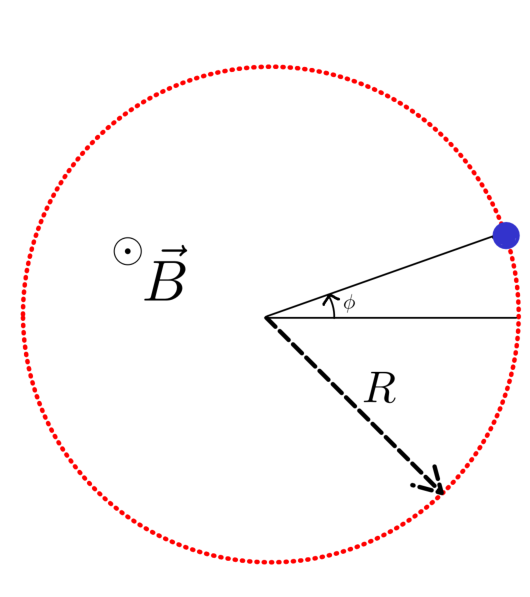
\includegraphics[width=0.3\linewidth]{particle-on-a-ring}
	\caption{A free particle on a ring. A magnetic field $\vec{B}$ is applied perpendicular to the plane of the ring.}
	\label{fig:particle-on-a-ring}
\end{figure}
While an wavepacket like that in Eq. \eqref{Eq:wavefunction-wavepacket} is localized around a point (say, $\vec{r}_0$), it the electron is not completely localized at that point, and can have an angular momentum due to the rotation about that point (in classical sense). As an analogy, if we could replace the electron probability density with the density of a classical charged fluid, that fluid could rotate about its center of mass, and would have an angular momentum due to that rotation, and consequently, a non-zero magnetic moment. We call this the orbital magnetic moment of an electron wavepacket,
\begin{equation}\label{Eq:OrbitalMagneticMomentExpression}
	\vec{m}_{\vec{k}} = -\frac{e}{2 m} \bra{\psi_{\vec{k}, \vec{r}_0}}(\hat{\vec{r}} - \vec{r}_0)\times\hat{\vec{p}}\ket{\psi_{\vec{k}, \vec{r}_0}}
\end{equation}
This is just a generalization of the formula $\vec{m} = (-e)g \frac{\vec{L}}{2 m}$, with the Lande-$g$ factor set to 1, as this magnetic moment is due to the spatial motion of the electron, and not due to its spin angular momentum.
Note that $m$ is the bare electron mass (not the effective mass of a Bloch state).\footnote{See Appendix \ref{app:mass-of-wavepackets} for some discussion on the mass present in different relations.}

\subsection{An example}

For a free electron moving in a ring of radius $R$ (Fig. \ref{fig:particle-on-a-ring}), the eigenfunctions of the Hamiltonian are $\psi_n(\phi) = \frac{1}{2 \pi R} e^{i n \phi}$, with energy eigenvalue, $\varepsilon_{0}(n) = \frac{\hbar^2 n^2}{2 m R^2}$ It has an orbital angular momentum $n\hbar$ about the center of the ring, and a magnetic moment $m_z = -\frac{e}{2m} n\hbar$.
When a magnetic field perpendicular to the center of mass is applied, the eigenfunctions remain the same, but the energy eigenvalues are modified to,
$\varepsilon(n) = \frac{1}{2 m R^2} (n\hbar + \frac{eBR^2}{2})^2$. Then, up to linear order in the magnetic field, the energy eigenvalue is, $\varepsilon(n) = \frac{1}{2 m R^2} (n^2\hbar^2 + n \hbar eBR^2) = \varepsilon_{0}(n) - m_z B$.


While the density of this wavefunction is spread over all the ring, we can consider a localized wavepacket with the most significant contribution from this wavefunction, and that wavepacket would have almost the same magnetic moment, and the same energy eigenvalue.

\section{Is the orbital magnetic moment caused by the Berry Curvature?}
\textbf{No}. Consider a free particle moving in a ring. The eigenfunctions would have zero Berry curvature, but there is a net magnetic moment.
\section{Modified Expression for Electric Current Density}
Let us look back and try to see why we got an apparent violation of the Einstein and Onsager relations for the Anomalous Hall Effect, in Section \ref{sec:Einstein-Onsager-violation}. In the anomalous Hall effect, we got a term like $\vec{E} \times \int d\vec{k} \vec{\Omega}(\vec{k}) $, but there were no terms like $\nabla \mu \times \vec{\Omega}(\vec{k}) $, or $\nabla T \times \vec{\Omega}(\vec{k}) $. The electric field enters through the solution of the semiclassical equation o f velocity, whereas the gradient of the chemical potential and the gradient of the temperature entered through the out of equilibrium part of the distribution function.

To get this term, we need to use the statement that the wavepacket has a finite width, an electron in a Bloch wavepacket centered at $\vec{r}_0$ can be found at $\vec{r}_1 \neq \vec{r}_0$, and it can contribute to the current at $\vec{r}_1$ ($\neq \vec{r}_0$). As an analogy, the total electron density near an atom in a insulator is not just the electron density of that atom, but the sum of electron densities belonging to all the atoms, evaluated at that point. Of course, atoms far away from the point would contribute very less, but nearby atoms can contribute significantly. Previously, when we calculated $\expval{j}(\vec{r}_1)$, we only considered the contribution of the  Bloch wavepacket localized at $\vec{r}$.

Let us try to find the expectation value of a general operator $\mathcal{O}$ at a point $\vec{r}_1$. We would consider the sum of the contributions of all wavepackets centered at a point $\vec{r}_0$, and sum over all $\vec{r}_0$ \cite{XiaoElecPropertiesReview2010}. That is,

$$
	\expval{\hat{\mathcal{O}}}(\vec{r}_1) = \int d\vec{r}_0 \int  \frac{d\vec{k}}{(2\pi)^d} (f+g) (1+\frac{e}{\hbar} \vec{B}\cdot\vec{\Omega})
	\bra{\psi_{\vec{k},\vec{r}_0}} \frac{1}{2}\{\hat{\mathcal{O}}, \delta(\vec{\hat{r}} - \vec{r}_1)\} \ket{\psi_{\vec{k},\vec{r}_0}} 
$$
Here $\vec{\hat{r}}$ is the position operator that acts on the states. $\vec{r}_1$ is just a parameter, and here $\vec{r}_1$ acting on a state has to be understood as the operator $\vec{r}_1 \mathcal{I}$, with $\mathcal{I}$ being the identity operator acting on the Hilbert space. And,
$\frac{1}{2}\{\hat{\mathcal{O}}, \delta(\vec{\hat{r}} - \vec{r}_0)\}$ denotes the Hermitized operator $\frac{\hat{\mathcal{O}}  \delta(\vec{\hat{r}} - \vec{r}_1) + \delta(\vec{\hat{r}} - \vec{r}_1)\hat{\mathcal{O}}  }{2}$, in case $\hat{\vec{r}}$ and $\hat{\mathcal{O}}$ does not commute. $\ket{\psi_{\vec{k},\vec{r}_0}}$ is the Bloch wavepacket with the expectation values of position and crystal momentum being $\vec{r}_0$, and $\vec{k}$, respectively.

Now, since the state is spread around $\vec{r}_0$, we can take that into account by expanding the delta function (up to leading order),
$$
\delta(\vec{r}_1 - \vec{\hat{r}}) = \delta((\vec{r}_1 - \vec{r}_0) - (\vec{\hat{r}} - \vec{r}_0)) \approx \delta(\vec{r}_1 - \vec{r}_0) - (\vec{\hat{r}} - \vec{r}_0) \cdot \nabla_{\vec{r}_1} \delta(\vec{r}_1 - \vec{r}_0)
$$
Using this, we get,
\begin{equation}\label{Eq:expectation-value-of-general-operator-O}
	\begin{aligned}
	\expval{\hat{\mathcal{O}}}(\vec{r}_1) &= \int  \frac{d\vec{k}}{(2\pi)^d} (f+g) (1+\frac{e}{\hbar} \vec{B}\cdot\vec{\Omega})
	\bra{\psi_{\vec{k},\vec{r}_1}} \hat{\mathcal{O}} \ket{\psi_{\vec{k},\vec{r}_1}} \\
	& -\nabla_{\vec{r}_1} \cdot \int \frac{d\vec{k}}{(2\pi)^d} (f+g) (1+\frac{e}{\hbar} \vec{B}\cdot\vec{\Omega})
	\bra{\psi_{\vec{k},\vec{r}_1}} \frac{1}{2}\{\hat{\mathcal{O}}, (\vec{\hat{r}} - \vec{r}_1)\} \ket{\psi_{\vec{k},\vec{r}_1}} 
	\end{aligned} 
\end{equation}
We would work with this leading order expansion of the Delta function. For the current density operator, we need to separately take the three components of $\vec{\hat{j}} = -e\frac{\hat{\vec{p}}}{m}$ to be $\hat{\mathcal{O}}$.

Let us define the tensor,
$$\mathcal{M}_{i,j} = \bra{\psi_{\vec{k},\vec{r}_1}} \frac{1}{2}\{-e\frac{\hat{p}_j}{m}, (\vec{\hat{r}} - \vec{r}_1)_i\} \ket{\psi_{\vec{k},\vec{r}_1}} 
$$
where $i,j$ runs from $1,2, \dots d$. It can be shown that (see Appendix \ref{app:all-about-mag-mom}) $\mathcal{M}_{i,j}$ is completely antisymmetric \cite{PhysRevLett.124.066601}. Then, in 3D universe (the sample can still be 2 dimensional), we can construct a vector, whose components are, $m_i = \frac{1}{2} \epsilon_{ijk} \mathcal{M}_{j k}$ (\cite{PhysRevLett.124.066601}). It can be shown (see Appendix \ref{app:all-about-mag-mom}) that this is nothing but the orbital magnetic moment, defined in Eq. \eqref{Eq:OrbitalMagneticMomentExpression}. We can also invert the relation, $\mathcal{M}_{jk} = m_i \epsilon_{ijk}$.

Note that we can rewrite the new term as,
$$
\begin{aligned}
&-\nabla_{\vec{r}_1} \cdot \int \frac{d\vec{k}}{(2\pi)^d} (f+g) (1+\frac{e}{\hbar} \vec{B}\cdot\vec{\Omega})
\bra{\psi_{\vec{k},\vec{r}_1}} \frac{1}{2}\{\hat{\mathcal{O}}, (\vec{\hat{r}} - \vec{r}_1)\} \ket{\psi_{\vec{k},\vec{r}_1}}\\ &= -\partial_i \int \frac{d\vec{k}}{(2\pi)^d} (f+g) (1+\frac{e}{\hbar} \vec{B}\cdot\vec{\Omega})
\bra{\psi_{\vec{k},\vec{r}_1}} \frac{1}{2}\{\hat{\mathcal{O}}, (\vec{\hat{r}} - \vec{r}_1)_i\} \ket{\psi_{\vec{k},\vec{r}_1}},
\end{aligned}$$ with sum over $i$ implied. Then to get the $\mu$-th component of $\expval{\vec{\hat{j}}}$, we take $\mathcal{\hat{O}} = -e\frac{\hat{{p}_\mu}}{m}$. We denote $[dk] = \frac{d\vec{k}}{(2\pi)^d} (1+\frac{e}{\hbar} \vec{B}\cdot\vec{\Omega})$. We get,
$$\begin{aligned}
	&-\partial_i \int [dk] (f+g) \mathcal{M}_{i \mu}\\
&= -\partial_i \int [dk] (f+g) m_{\nu} \epsilon_{\nu i \mu}\\
&= +\partial_i \int [dk] (f+g) m_{\nu} \epsilon_{ i \nu \mu}
\end{aligned}
$$
This is the $\mu$-th component of $\nabla \times \int \frac{d\vec{k}}{(2\pi)^d} (f+g) (1+\frac{e}{\hbar} \vec{B}\cdot\vec{\Omega}) \vec{m}_{\vec{k}}$. When the electric field, chemical potential gradient and the temperature gradients are constant, we can drop the term $\nabla \times \int d\vec{k} g (1+\frac{e}{\hbar} \vec{B}\cdot\vec{\Omega}) \vec{m}_{\vec{k}}$, because $g$ is already a linear function of $\vec{E}$, $\nabla \mu$ and $\nabla T$.

Finally we get,
\begin{equation}~\label{Eq:electric-current-simplified-magnetization-included}
	\expval{\hat{\vec{j}}_e} = -e \int \frac{d\vec{k}}{(2\pi)^d} {g}_{\vec{k}} \frac{1}{\hbar} \frac{\partial \varepsilon_{_{\vec{k}}}}{\partial \vec{k}} + {f}_{\vec{k}} \frac{e}{\hbar} (\vec{E} \times \vec{\Omega}(\vec{k})) + \nabla \times \int \frac{d\vec{k}}{(2\pi)^d} f_{\vec{k}} \left(1+\frac{e}{\hbar} \vec{B}\cdot\vec{\Omega}\right) \vec{m}_{\vec{k}}.
\end{equation}
This equation has a simple interpretation. The net current is the contribution of the center of mass movements of the wavepackets, as well as due to the rotation about their individual centers of mass.
We want to calculate the properties of the anomalous Hall effect, where $\vec{B} = 0$. Then the expression simplifies to \begin{equation}~\label{Eq:electric-current-simplified-magnetization-included-zeromagfield}
	\left. \expval{\hat{\vec{j}}_e}\right|_{\vec{B} = 0} 
	= -e \int \frac{d\vec{k}}{(2\pi)^d} {g}_{\vec{k}} \frac{1}{\hbar} \frac{\partial \varepsilon_0({{\vec{k}}})}{\partial \vec{k}} + {f}_{\vec{k}} \frac{e}{\hbar} (\vec{E} \times \vec{\Omega}(\vec{k})) + \nabla \times \int \frac{d\vec{k}}{(2\pi)^d} f_{\vec{k}}  \vec{m}_{\vec{k}}.
\end{equation}

\section{Total Magnetization of the system}
Due to the orbital moment of the Bloch wavepackets, the system gets a net non-zero magnetization, which leads to circulating along its edges.
However, the net magnetization density is slightly different from the sum of the individual orbital magnetic moments. This is because, the phase space density changes when as we turn on a magnetic field (even in the limit of a zero magnetic field, see the expression of $\vec{M}^e$ below).
Under zero external electric field, and zero chemical potential gradient and temperature gradient, the Gibbs free energy of the system is \cite{PhysRevLett.97.026603}, 

$\begin{aligned}
G &= -\frac{1}{\beta} \sum_{\vec{k}} \log(1 + e^{-\beta(\varepsilon_{_{\vec{k}}} - \vec{m}_{\vec{k}}\cdot \vec{B} - \mu)}) \\
&= -\frac{1}{\beta} \int  \frac{d\vec{k}}{(2\pi)^d} \left(1+\frac{e}{\hbar} \vec{B}\cdot\vec{\Omega}\right) \log(1 + e^{-\beta(\varepsilon_{_{\vec{k}}} - \vec{m}_{\vec{k}}\cdot \vec{B} - \mu)})
\end{aligned}$

Then the magnetization is,
\begin{equation}\label{Eq:electric-magnetization}
	\begin{aligned}
		\vec{M}^e &= \left.\frac{\partial G}{\partial \vec{B}}\right|_{\vec{B}=0} \\
		&= \frac{1}{\beta} \int  \frac{d\vec{k}}{(2\pi)^d}  \frac{e}{\hbar} \vec{\Omega}(\vec{k}) \log(1 + e^{-\beta(\varepsilon_0(\vec{k}) - \mu)}) + \int  \frac{d\vec{k}}{(2\pi)^d} f \vec{m}_{\vec{k}}
	\end{aligned}
\end{equation}
The circulating magnetization current is,
\begin{equation}
\begin{aligned}
	\vec{j}^e_M &= \nabla \times \vec{M}^e \\
	&= \nabla \times \int \frac{d\vec{k}}{(2\pi)^d} f \vec{m}_{\vec{k}} + \nabla \mu \times \int  \frac{d\vec{k}}{(2\pi)^d} \frac{e}{\hbar} \vec{\Omega}(\vec{k}) f + \frac{\nabla T}{T}  \times \int  \frac{d\vec{k}}{(2\pi)^d} \frac{e}{\hbar} \vec{\Omega}(\vec{k}) f_{\vec{k}} (\varepsilon_0(\vec{k}) - \mu) \\
	&+ \frac{\nabla T}{T}  \times \int  \frac{d\vec{k}}{(2\pi)^d} \frac{e}{\hbar} \vec{\Omega}(\vec{k}) k_B T \log(1 + e^{-\beta(\varepsilon_0(\vec{k}) - \mu)})
\end{aligned}
\end{equation}
We cannot measure this circulating magnetization current in transport experiments, what we measure is the transport current, which is obtained by subtracting the magnetization current from the total current,
\begin{equation}~\label{Eq:transport-electric}
	\boxed{\begin{aligned}
	{{\vec{j}}^e}_{\text{transport}} &= \expval{\hat{\vec{j}}_e} - {\vec{j}^e}_{M} \\
	&= \int \frac{d\vec{k}}{(2\pi)^d} (-e){g}_{\vec{k}} \frac{1}{\hbar} \frac{\partial \varepsilon_0({{\vec{k}}})}{\partial \vec{k}} - {f}_{\vec{k}} \frac{e^2}{\hbar} \left(\left[\vec{E} + \frac{\nabla \mu}{e} \right] \times \vec{\Omega}(\vec{k})\right) \\
	&- \frac{\nabla T}{T}  \times \int  \frac{d\vec{k}}{(2\pi)^d} \frac{e}{\hbar} \vec{\Omega}(\vec{k}) \left[f_{\vec{k}} (\varepsilon_0(\vec{k}) - \mu) + k_B T \log(1 + e^{-\beta(\varepsilon_0(\vec{k}) - \mu)})\right]
	\end{aligned}}
\end{equation}
We now see that the \textit{Einstein relation} is valid because we can exchange $\vec{E} \leftrightarrow \frac{\nabla \mu}{e}$ (the validity of the Einstein relation in the non-equilibrium distribution $g_{\vec{k}}$ has already been shown in section \ref{sec:non-eq-Einstein-Onsager}). To show that the Onsager relation is valid, we need to find the modified expression of the heat current, taking into account of the magnetization density.

\section{Modified Expression for Heat Current Density}
We can use a similar approach for the heat current density, and it can be shown that \cite{PhysRevLett.97.026603} the total heat current is,
\begin{equation} \label{Eq:heat-current-simplified-including-magnetization}
	\expval{\hat{\vec{j}}_Q} = \int \frac{d\vec{k}}{(2\pi)^d} (\varepsilon_0(\vec{k}) - \mu) \left[ {g}_{\vec{k}} \frac{1}{\hbar} \frac{\partial \varepsilon_0(\vec{k})}{\partial \vec{k}} + \frac{e}{\hbar} {f}_{\vec{k}} (\vec{E}\times\vec{\Omega}(\vec{k}))\right]
	- \vec{E} \times \int \frac{d\vec{k}}{(2\pi)^d}
	 f_{\vec{k}} \vec{m}_{\vec{k}}
\end{equation}
Here the magnetic field has been set to zero, and terms up to linear order in Electric field has been taken. This is the total energy current density, and is the sum of transport and magnetization energy currents. Just like the case of electric current, the magnetization current is the curl of energy magnetization, which is \cite{CooperHalperin1997}, $\vec{M}^E = \vec{M}_0^E + \phi(\vec{r}) \vec{M}^N$. Here $\vec{M}_0^E$ is the energy magnetization at zero electric field (we call it the bare energy magnetization), and $\vec{M}^N$ is the number density magnetization (whose curl is the number current density, i.e. the electric current density divided by the electric charge), and $\phi(\vec{r}) = e \vec{E} \cdot \vec{r}$ is the potential energy due to the electric field. In presence of an electric field, we need to add this additional term because the charges would carry the potential energy. Both the bare energy magnetization $\vec{M}_0^E$ and the number density magnetization $\vec{M}^N = \frac{\vec{M}^e}{-e}$ are functions of the chemical potential $\mu$ and temperature $T$. Then we can rewrite the energy magnetization as, $\vec{M}^E = \vec{M}_0^E - (\vec{E}\cdot\vec{r}) \vec{M}^e$. Here $\vec{M}_0^E$

Then, the magnetization energy current density is,
$$
\begin{aligned}
	\vec{j}^E_M = \nabla \times \vec{M}_0^E - \vec{E} \times \vec{M}^e - \underbrace{(\vec{E} \cdot \vec{r}) \nabla \times \vec{M}^e}_{\text{2nd order quantity}}
\end{aligned}
$$
Here $\nabla \times \vec{M}^e$ is already a function of $\nabla \mu$ and $\nabla T$, and the term $(\vec{E} \cdot \vec{r}) \nabla \times \vec{M}^e$ is of the second order, and we drop it. It follows that, 
$$\begin{aligned}
	\vec{j}^E_M &= \nabla \mu \times \frac{\partial \vec{M}_{0}^{E}}{\partial \mu}+\nabla T \times \frac{\partial \vec{M}_{0}^{E}}{\partial T}-\vec{E} \times \vec{M}^{e}\\
	&= \nabla \mu \times \frac{\partial \vec{M}_{0}^{E}}{\partial \mu}+\nabla T \times \frac{\partial \vec{M}_{0}^{E}}{\partial T} -\vec{E} \times \int \frac{d\vec{k}}{(2\pi)^d} \vec{m}(\vec{k}) f_{k}+k_{B} T \frac{e \vec{\Omega}}{\hbar} \log(1 + e^{-\beta(\varepsilon_0(\vec{k}) - \mu)})
\end{aligned}$$
Then, the transport energy current density is,
$$
\begin{aligned}
	\vec{j}_{\text {transport }}^{E} &=\vec{j}_{\text {total }}^{E}-\nabla \times \vec{M}^{E} \\
	&=\int \frac{d\vec{k}}{(2\pi)^d} \varepsilon_0(\vec{k}) \left[ {g}_{\vec{k}} \frac{1}{\hbar} \frac{\partial \varepsilon_0(\vec{k})}{\partial \vec{k}} + \frac{e}{\hbar} {f}_{\vec{k}} (\vec{E}\times\vec{\Omega}(\vec{k}))\right] \\
	& + \vec{E} \times \int \frac{d\vec{k}}{(2\pi)^d}k_{B} T \frac{e \vec{\Omega}}{\hbar} \log(1 + e^{-\beta(\varepsilon_0(\vec{k}) - \mu)}) -\nabla \mu \times \frac{\partial \vec{M}_{0}^{E}}{\partial \mu}-\nabla T \times \frac{\partial \vec{M}_{0}^{E}}{\partial T}
\end{aligned}
$$
And the transport heat current density is,
\begin{equation}\label{Eq:heat-current-density-transport}
	\boxed{\begin{aligned}
	\vec{j}_{\text {transport }}^{Q} &=\vec{j}_{\text {transport }}^{E}-\mu \vec{j}_{\text {transport }}^{N}  = \vec{j}_{\text {transport }}^{E}-\frac{\mu}{-e} \vec{j}_{\text {transport }}^{e}\\
	&=\int \frac{d\vec{k}}{(2\pi)^d}(\varepsilon_0(\vec{k})-\mu) \frac{1}{\hbar} \frac{\partial \varepsilon_0(\vec{k})}{\partial \vec{k}} g_{k} \\
	&+\vec{E} \times \int \frac{d\vec{k}}{(2\pi)^d} \left[(\varepsilon_0(\vec{k})-\mu) \frac{e}{\hbar} \vec{\Omega} f_{k} + k_{B} T \frac{e \vec{\Omega}}{\hbar} \log(1 + e^{-\beta(\varepsilon_0(\vec{k}) - \mu)})\right] \\
	&+ \int \frac{d\vec{k}}{(2\pi)^d} (-\mu) \frac{1}{\hbar} \nabla \mu \times \vec{\Omega} f_{k} \\
	&-\frac{\mu}{\hbar} \int \frac{d\vec{k}}{(2\pi)^d} \frac{\nabla T}{T} \times \vec{\Omega}\left[f_{k}\left(\varepsilon_0(\vec{k})_{k}-\mu\right)+k_{B} T \log(1 + e^{-\beta(\varepsilon_0(\vec{k}) - \mu)})\right] \\
	&-\nabla \mu \times \frac{\partial \vec{M}_{0}^{E}}{\partial \mu}-\nabla T \times \frac{\partial \vec{M}_{0}^{E}}{\partial T}
\end{aligned}}
\end{equation}
\subsection{Validity of the Onsager relation, and the Einstein relation in the heat current density}
\subsubsection{Einstein Relation}
In the second and third terms, there is some asymmetry between $e \vec{E}$ and $\nabla \mu$. For the \textit{Einstein relation} (symmetry between $e \vec{E}$ and $\nabla \mu)$ to hold, we must have a term like $$(e\vec{E} + \nabla \mu) \times \int \frac{d\vec{k}}{(2\pi)^d}  \frac{ \vec{\Omega}}{\hbar} \left[(\varepsilon_0(\vec{k})-\mu) f_{k} + k_{B} T \log(1 + e^{-\beta(\varepsilon_0(\vec{k}) - \mu)})\right].$$
The missing terms must come from $-\nabla \mu \times \frac{\partial \vec{M}_{0}^{E}}{\partial \mu}$. 

We must have, for Einstein relation to hold, 

$-\nabla \mu \times \frac{\partial \vec{M}_{0}^{E}}{\partial \mu} =  \nabla \mu \times \int \frac{d\vec{k}}{(2\pi)^d}  \frac{ \vec{\Omega}}{\hbar} \left[\varepsilon_0(\vec{k}) f_{k} + k_{B} T \log(1 + e^{-\beta(\varepsilon_0(\vec{k}) - \mu)})\right]$,
i.e., 
\begin{equation}\label{Eq:energy-mag-condition}
	\boxed{-\frac{\partial \vec{M}_{0}^{E}}{\partial \mu}=\int \frac{d\vec{k}}{(2\pi)^d}  \frac{ \vec{\Omega}}{\hbar} \left[\varepsilon_0(\vec{k}) f_{k} + k_{B} T \log(1 + e^{-\beta(\varepsilon_0(\vec{k}) - \mu)})\right]}
\end{equation}

\subsubsection{Onsager Relation}
We have already seen in section (\ref{sec:non-eq-Einstein-Onsager}) that the Onsager relation is valid for the non-equilibrium distribution. For the equilibrium distribution, in the expression of $\vec{j}_{\text {transport }}^{Q}$ (Eq. \eqref{Eq:heat-current-density-transport}), we have the term, $\vec{E} \times \int \frac{d\vec{k}}{(2\pi)^d} \left[(\varepsilon_0(\vec{k})-\mu) \frac{e}{\hbar} \vec{\Omega} f_{k} + k_{B} T \frac{e \vec{\Omega}}{\hbar} \log(1 + e^{-\beta(\varepsilon_0(\vec{k}) - \mu)})\right]$, and in the expression of $\vec{j}_{\text {transport }}^{e}$ (Eq. \eqref{Eq:transport-electric}), we had, $-\frac{\nabla T}{T}  \times \int  \frac{d\vec{k}}{(2\pi)^d} \frac{e}{\hbar} \vec{\Omega}(\vec{k}) \left[f_{\vec{k}} (\varepsilon_0(\vec{k}) - \mu) + k_B T \log(1 + e^{-\beta(\varepsilon_0(\vec{k}) - \mu)})\right]$, and the Onsager relation is valid for the terms contributing to $\stackrel{\leftrightarrow}{L}_{12}$ and $\stackrel{\leftrightarrow}{L}_{21}$.

\chapter{Seebeck, Peltier and Nernst effects}~\label{chap:Seebeck-Peltier-Nernst}
In this chapter, we would review various thermoelectric effects. In this chapter, the discussion about Seebeck and Peltier effect are based on that in chapter 13 of \cite{book:AshcroftMermin76}.
\section{Seebeck Effect and Thermopower}

Suppose, we have two metal wires clamped together in one end, which is maintained at $T_1$, and the other end of both the metals is maintained at $t_0$. The temperature gradient will try to cause an electric current, but here there cannot be any electric current as the circuit is open. Due to the temperature gradient, the electrons would accumulate at the edges of the system, and there would be an internal electrochemical field, $\vec{\xi} = \vec{E} + \frac{1}{e} \nabla \mu$ due to them.
\begin{figure}[h!]
	\centering
	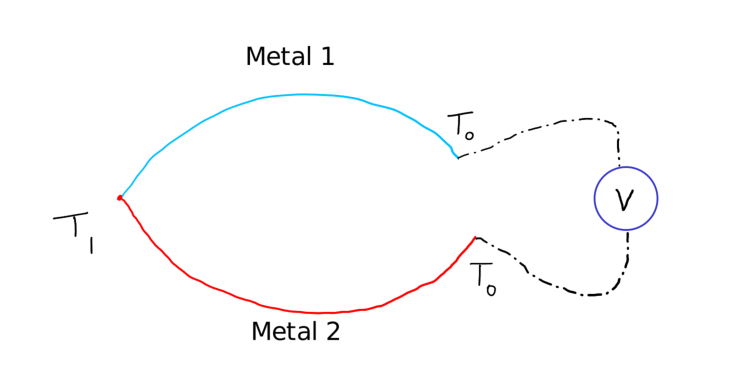
\includegraphics[width=0.7\linewidth]{seebeck}
	\caption{An illustration of Seebeck effect. The two ends are kept at constant temperatures $T_0$ and $T_1$, and a voltage is generated.}
	\label{fig:seebeck}
\end{figure}


We can measure the E.M.F. generated with a voltmeter, and experimentally, $\int_{\text{low temp}}^{\text{high temp}} \vec{\xi} \cdot d \vec{l} = Q \Delta T$, where $Q$ is known as the thermopower, or the Seebeck coefficient. We can rewrite $\Delta T = \int_{\text{low temp}}^{\text{high temp}} \nabla T \cdot d\vec{l}$.

Then, we can write, $\vec{\xi} = Q \nabla T$.

Since the electric current is zero, $\vec{j}=  \stackrel{\leftrightarrow}{L}_{11} \cdot \left(\vec{E} + \nabla \frac{\mu}{e}\right) + \stackrel{\leftrightarrow}{L}_{12} \cdot (-\nabla{T}) = 0$.

Then, $\stackrel{\leftrightarrow}{Q} = \vec{\xi} \cdot (\nabla T)^{-1} = {\stackrel{\leftrightarrow}{L}}^{-1}_{11} \stackrel{\leftrightarrow}{L}_{12}$.

\section{Peltier Effect}
Suppose, a circuit is made of two metallic plates, and a uniform electric current $\vec{j}_e$ is made through to through it, using a battery. Due to the electric field of the battery, there must be a heat current $\vec{j}_Q$, which would be different in the two metals. As a result, there would be accumulation of heat in one of the junction, and heat would evolve at another. We can couple this system to external reservoirs so that heat can be supplied at one junction, and dissipated at another. If the battery is connected as shown in the figure, we can assume that there would be negligible heat current through the lower plate, as there is a disconnection in between.
\begin{figure}[h!]
	\centering
	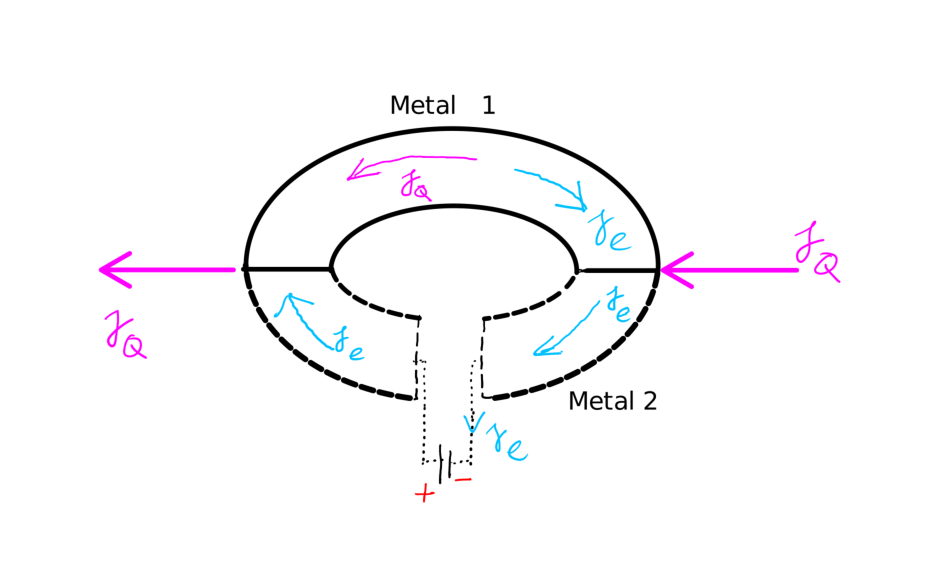
\includegraphics[width=0.7\linewidth]{peltier}
	\caption{An illustration of the Peltier Effect}
	\label{fig:peltier}
\end{figure}

Experimentally, it is found that $\vec{j}_Q = \stackrel{\leftrightarrow}{\Pi} \cdot \vec{j}_e$, where $\stackrel{\leftrightarrow}{\Pi}$ is the Peltier coefficient.

Since there is a uniform temperature, $\nabla T = 0$.

Then, with the relations $$\vec{j}_e = \stackrel{\leftrightarrow}{L}_{11} \cdot \left(\vec{E} + \nabla \frac{\mu}{e}\right) + \stackrel{\leftrightarrow}{L}_{12} \cdot (-\nabla{T}),$$  
$$\vec{j}_Q = \stackrel{\leftrightarrow}{L}_{21} \cdot \left(\vec{E} + \nabla \frac{\mu}{e}\right)  + \stackrel{\leftrightarrow}{L}_{22} \cdot (-\nabla{T}),$$ and $\nabla T = 0$, we find that $\stackrel{\leftrightarrow}{\Pi} =  \stackrel{\leftrightarrow}{L}_{21} {\stackrel{\leftrightarrow}{L}}^{-1}_{11}$.

From the Onsager relation, $\stackrel{\leftrightarrow}{L}_{21} = T \stackrel{\leftrightarrow}{L}_{12}$. Then, if $\stackrel{\leftrightarrow}{L}_{11}$ and $\stackrel{\leftrightarrow}{L}_{12}$ commute, it follows that $$\boxed{\stackrel{\leftrightarrow}{\Pi} =  T \stackrel{\leftrightarrow}{Q}}.$$

This relation between the Peltier and the Seebeck coefficient was first deduced by Lord Kelvin.
\section{Nernst Effect}
In Hall effect, an electric field generates a current, and a perpendicular magnetic field tries to rotate the direction of the current. However, since electrons cannot leave the sample, they accumulate at the edges, and an electrochemical field is set up, perpendicular to both the magnetic field and the original electric field. This electrochemical field leads to a Hall voltage, which can be measured.

In the previous sections we saw that a temperature gradient can give rise to electric current, just like an electric field. Then, if apply a temperature gradient, and a magnetic field perpendicular to that, we would expect a Hall-like voltage generated in the direction perpendicular to both the magnetic field and the temperature gradient. This is known as the Nernst effect.

Suppose, a temperature gradient $-\nabla T \hat{x}$ is set up, and a magnetic field $B \hat{z}$ is applied. And, the sample is connected to electrically insulating heat conductors in both side. Then, the $x$ and $y$ components of $\vec{j}_e$ would both be $0$.

Since ${\vec{j}_e}_x = 0$, $\sigma_{xx} \xi_x + \sigma_{xy} \xi_y + \alpha_{xx} (-\nabla T)_x = 0$. 

Since ${\vec{j}_e}_y = 0$, $\sigma_{yx} \xi_x + \sigma_{xx} \xi_y + \alpha_{y x} (-\nabla T)_x = 0$ (since $\sigma_{xx} = \sigma_{yy}$ in an isotropic sample).

Eliminating $\xi_x$ from the two equations, and using the relations $\alpha_{y x} = \alpha_{x y}$, and $\sigma_{y x} = \sigma_{x y}$, we get, $\frac{\xi_y}{(-\nabla T)_x} = \frac{\sigma_{xx} \alpha_{xy} - \sigma_{xy} \alpha_{xx}}{\sigma_xx ^2 + \sigma_xy ^2}$.

The Nernst response is defined \cite{Ussishkin_2002} as,
$$\nu = \frac{1}{B} \frac{\xi_y}{(-\nabla T)_x} = \frac{1}{B} \frac{\sigma_{xx} \alpha_{xy} - \sigma_{xy} \alpha_{xx}}{\sigma_{xx} ^2 + \sigma_{xy} ^2}.$$



\subsection{Anomalous Nernst Effect}
Just like anomalous Hall effect, the Berry curvature can create off diagonal response in absence of a magnetic field, resulting in an anomalous Nernst response,
$$\nu_\text{anomalous} = \frac{\xi_y}{(-\nabla T)_x} = \frac{\sigma_{xx} \alpha_{xy} - \sigma_{xy} \alpha_{xx}}{\sigma_{xx} ^2 + \sigma_{xy} ^2}.$$

In presence of Berry Curvature, $\alpha_{xy}$ and $\sigma_{xy}$ can be non-zero, and there can be a non-zero Nernst response, as long as time reversal symmetry is broken, either intrinsically, or by applying an circularly polarized electromagnetic wave.

It has been shown that the anomalous Nernst effect is also quantized \cite{QuantizedNernstNoky_2021}.
\chapter{Calculation of Berry Curvature and Chern Number in various models}\label{chap:ChernNumber}
We saw that the Anomalous Hall conductivity is proportional to the Chern Numner. In this section we would look at different systems, and discuss their Berry curvature and Chern numbers.
\section{Monolayer and Bilayer Graphene}
Graphene is a two dimensional sheet of Carbon atoms, arranged in a honeycomb lattice. It is actually a single layer of graphite, and indeed, graphene is created in lab by exfoliating a later of graphite with a scotch tape. Although previously used as a theoretical toy model, graphene was isolated and characterized by Geim and Novoselov et al. \cite{NovoselovGeimGraphene666} in 2004. It shows many wonderful electronic properties. Its band structure has a linear energy-momentum dispersion \cite{NovoselovGrapheneDirac2005} relation at certain points, like that of a massless relativistic particle. It can show integer, half-integer \cite{Zhang2005GrapheneQHEBerry} and fractional \cite{Bolotin2009GrapheneFQHE} Quantum Hall effects. Graphene is a semimetal. It has a gapless dispersion, but the density of states is zero at the band touching point.

We can stack two graphene sheets on top of each other, to form bilayer graphene and twist the two layers to some small angle. Twisted bilayer graphene can show superconductivity \cite{Cao2018TBLSuperconductivity} at some specific twist angles (e.g. $1.1^{\degree}$), known as magic angles.

\begin{figure}[h!]
	\centering
	\subfigure[]{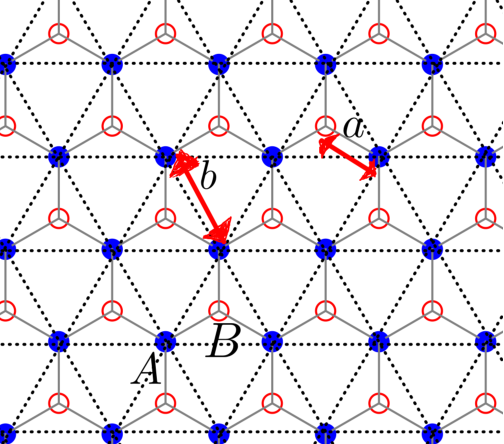
\includegraphics[width=0.3\linewidth]{graphene-lattice2.pdf}}
	\subfigure[]{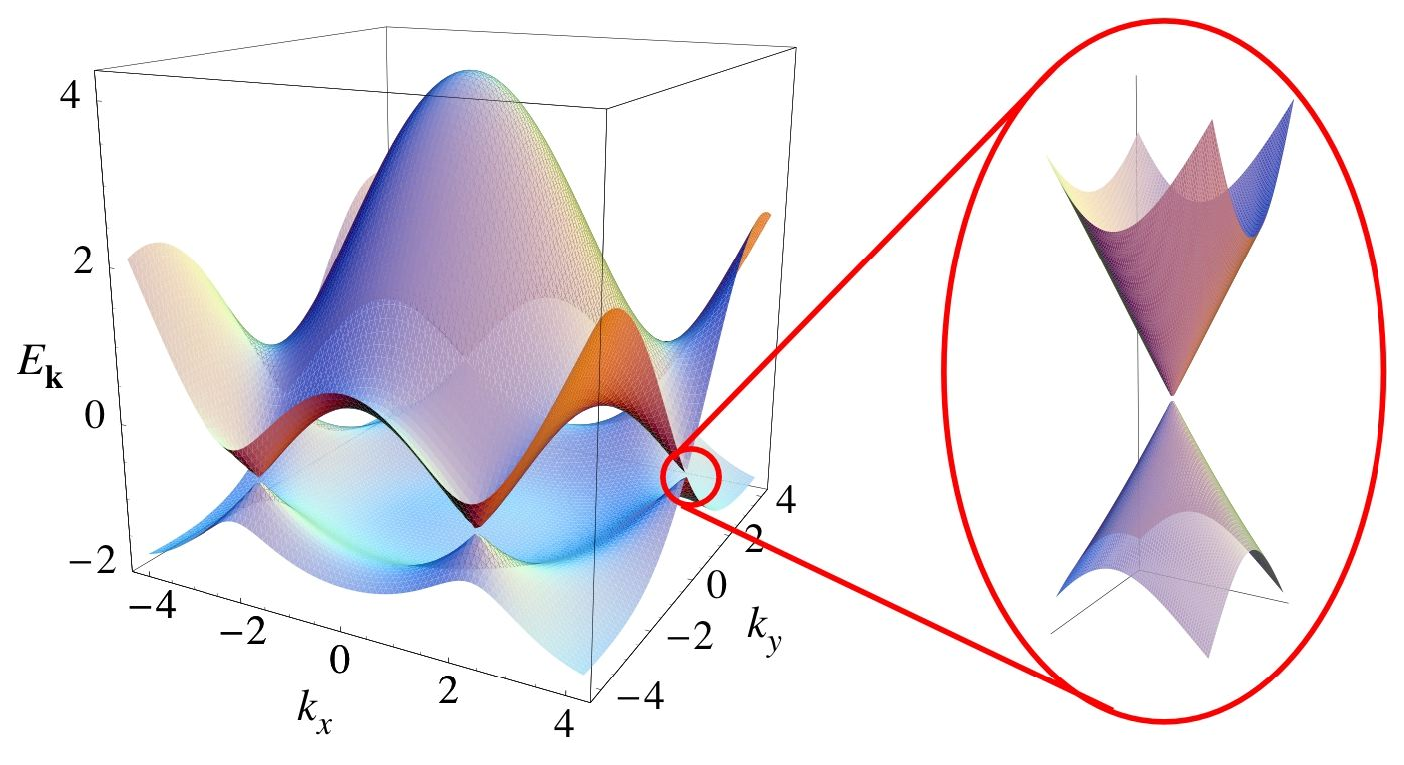
\includegraphics[width=0.5\linewidth]{Fig_dispersion_graphene.tl}}
	\caption{(a) Lattice structure of graphene. The blue sites are marked as A, and the red, hollow sites are marked as B. The distance between two carbon atoms is $a$, and the lattice constant of the triangular lattice is $b = 2 a \cos{30^{\degree}} = a\sqrt{3}$. (b) Band structure of monolayer Graphene. The Dirac cones near the $\vec{K}$ points has been shown in the inset. Figure reprinted with permissions from \cite{TheElPropGraphene}}
	\label{fig:GrapheneBandStructure}
\end{figure}

\subsection{Brillouin Zone and Band Structure}
The 2D hexagonal structure does not form a lattice because the sites labelled A and B do not feel the same environment around them. However, we can describe the periodic structure of the system in terms of a triangular lattice with a basis of A and B atoms \cite{book:SimonSolidState}. The Brillouin Zone is also hexagonal. Usually the origin of the reciprocal space is denoted as $\Gamma$. Among the six corners, any two next nearest corners can be connected by a reciprocal lattice vectors, and they are equivalent. As a result, only two of the six corners are independent. They are usually denoted by $\vec{K} (\frac{2\pi}{3b},\frac{2\pi}{\sqrt{3} b})$ and $\vec{K}'(\frac{4\pi}{3b},0)$. Experimentally, graphene shows linear dispersion about these points.

To calculate the band structure of monolayer graphene, we can use a tight binding model with nearest neighbor hopping and equal on-site energy on all the sites (which we can set to zero). Then the Hamiltonian is,
$H_0 = -t \sum_{\vec{R}} \sum_{\vec{r} \in {\text{nearest neighbors}}} \ket{B(\vec{r}+\vec{R})} \bra{A(\vec{R})} + h.c.$.

We can write this in the reciprocal space,
$$H_0 = -t \sum_{\vec{k}} \ket{\vec{k}}\bra{\vec{k}} \left[\sigma_x \left(1 + \cos(\frac{k_x b}{2} + \frac{k_y b \sqrt{3}}{2}) + \cos(k_x b)\right) + \sigma_y \left( \sin(\frac{k_x b}{2} + \frac{k_y b \sqrt{3}}{2}) + \sin(k_x b)\right)\right],$$
where $\ket{A} \equiv \begin{pmatrix}
1 \\
0 
\end{pmatrix}$, 
$\ket{B} \equiv \begin{pmatrix}
0 \\
1 
\end{pmatrix}$,
$\sigma_x = 
\begin{pmatrix}
	0 & 1 \\
	1 & 0
\end{pmatrix} \equiv \ket{A} \bra{B} + \ket{B} \bra{A}$, and 
$\sigma_y = 
\begin{pmatrix}
	0 & -i \\
	i & 0
\end{pmatrix} \equiv -i\ket{A} \bra{B} + i\ket{B} \bra{A}$.

The energy eigenvalues of a Hamiltonian of the form $H = \vec{d} \cdot \vec{\sigma}$ are $\pm \sqrt{d_x^2 + d_y^2 + d_z^2}$. Using this formula, we can calculate the energy eigenvalues,
$\varepsilon_{_{\vec{k}}}  = \pm t \sqrt{3 + 2 \cos{\frac{k_x b}{2}} \cos{(k_y b \frac{\sqrt{3}}{2})} + 2 \cos{k_x b}}$.

The bandstructure is plotted in Fig. \ref{fig:GrapheneBandStructure}. The energy eigenvalues become 0 at $\vec{K} (\frac{2\pi}{3b},\frac{2\pi}{\sqrt{3} b})$ and $\vec{K}'(\frac{4\pi}{3b},0)$ points. If we Taylor expand the energy eigenvalues about these points, the leading order terms are linear, $$\varepsilon_{q} = \left[\frac{\sqrt{3}}{2} t b\right] q,$$ where $\vec{q} = \left| \vec{k} - \vec{K} \right|$, or $\left| \vec{k} - \vec{K} \right|'$.

This dispersion is similar to that of a massless relativistic particle, and in two dimension, the energy-momentum relation forms a cone, termed as the Dirac cone (see Fig. \ref{fig:GrapheneBandStructure}(b)).

We can break the symmetry between the A, B sublattice points by introducing different on-site energies. This can be achieved by growing graphene on a Boron Nitride substrate, or by instead using a single layer Boron Nitride crystal instead (it also forms a hexagonal structure similar to graphene, with B and N atoms on the A and B sites, or vice versa.)

Then, the tight binding Hamiltonian would be,
$H = H_0 + \sum_{\vec{R}} \varepsilon_A \ket{A(\vec{R})} \bra{A(\vec{R})} + \varepsilon_B \ket{B(\vec{R})} \bra{B(\vec{R})}$. Leaving out the constant  $\frac{\varepsilon_A + \varepsilon_B}{2}$, we get,
\begin{equation}\label{Eq:GrapheneHopping}
	\begin{aligned}
H &=  \sum_{\vec{k}} \ket{\vec{k}}\bra{\vec{k}} [-t \sigma_x \left(1 + \cos(\frac{k_x b}{2} + \frac{k_y b \sqrt{3}}{2}) + \cos(k_x b)\right) \\
& -t \sigma_y \left( \sin(\frac{k_x b}{2}  + \frac{k_y b \sqrt{3}}{2}) + \sin(k_x b)\right)  + m \sigma_z ],
	\end{aligned}
\end{equation} with $m$ being $\frac{\varepsilon_A - \varepsilon_B}{2}$.

The dispersion about $\vec{K}$ or $\vec{K}'$ points would be, $\varepsilon_{q} = \sqrt{m^2 + \frac{3 t^2 b^2}{4} q^2} $, which is similar to $E = \sqrt{p^2 c^2 + m^2 c^4}$, the dispersion relation of a massive relativistic particle.

\subsection{Berry Curvature and Chern Number}
The Hamiltonian of any two-level system can be written as $\vec{d} \cdot \vec{\sigma}$, with $\vec{d} = (d_x, d_y, d_z)$ and $\vec{\sigma} = (\sigma_x, \sigma_y, \sigma_z)$. If $d_{x,y,z}$ are functions of $\vec{k}$, then the $z$ component of Berry curvature of the ground state can be written as (see \cite{shankar2018topological} for proof),
\begin{equation}\label{Eq:BerryTwoBandFormula}
	\Omega_z = 
	\frac{1}{2} \hat{d} \cdot \left(\frac{\partial \hat{d}}{\partial k_x} \times \frac{\partial \hat{d}}{\partial k_y} \right)
\end{equation}
(and cyclically exchange $x$, $y$, $z$ for other components).
Since the model has time reversal symmetry, $\vec{\Omega}(-\vec{k}) = -\vec{\Omega}(\vec{k})$, and the Chern number of monolayer graphene would be $0$, and there would be no anomalous Hall response.
\subsection{Selective Valley Population and Valley Chern Number}
While the Chern number of the whole Band is zero (it is also zero if the bands are partially populated, because in equilibrium, the two valleys would be equally populated, and they have opposite Berry curvatures), the valleys can be selectively populated \cite{valleyPolBilayerGraphene} with circularly polarized light.
Let us first see what is the Chern number of a single Dirac cone (stretched up to infinite momentum) is.
\subsubsection{Chern Number of a Single, Infinite Dirac Cone}
Consider the Hamiltonian $H(\vec{k}) = k_x \sigma_x + k_y \sigma_y + m \sigma_z$. It has a dispersion relation $\varepsilon_{_{\vec{k}}} = \pm \sqrt{k_x^2 + k_y^2 + m^2}$. Here $\vec{d} = (k_x, k_y, m)$. Using the formula in Eq. \eqref{Eq:BerryTwoBandFormula}, we get, $\vec{\Omega} = \frac{m}{2\left({k_x}^{2}+{k_y}^{2}+m^{2}\right)^{3 / 2}} \hat{z}$.
The corresponding Chern number is, $$\mathcal{C} = \frac{1}{2\pi} \int_{0}^{\infty} \frac{m}{2\left(k^2+m^{2}\right)^{3 / 2}} 2 \pi k dk = \frac{1}{2}.$$
This fractional Chern number is not of much concern, because we are not integrating over a closed, periodic surface.

Note that $\mathcal{C} = 0$ for $m = 0$, but it is $\frac{1}{2}$ for any finite but non-zero $m$.

If we look at the other band, its Berry curvature and Chern numbers would be exactly the negative of that obtained in this band.
\subsection{Chern Number of a Single Valley in the Brillouin Zone of monolayer graphene}

\begin{figure}[h!]
	\centering
	\subfigure[]{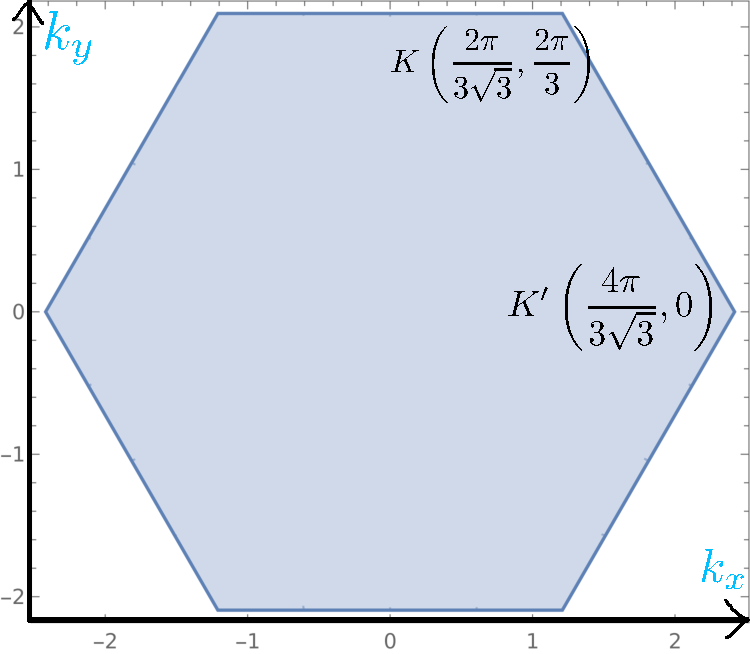
\includegraphics[width=0.35\linewidth]{fullBZ.pdf}}
	\subfigure[]{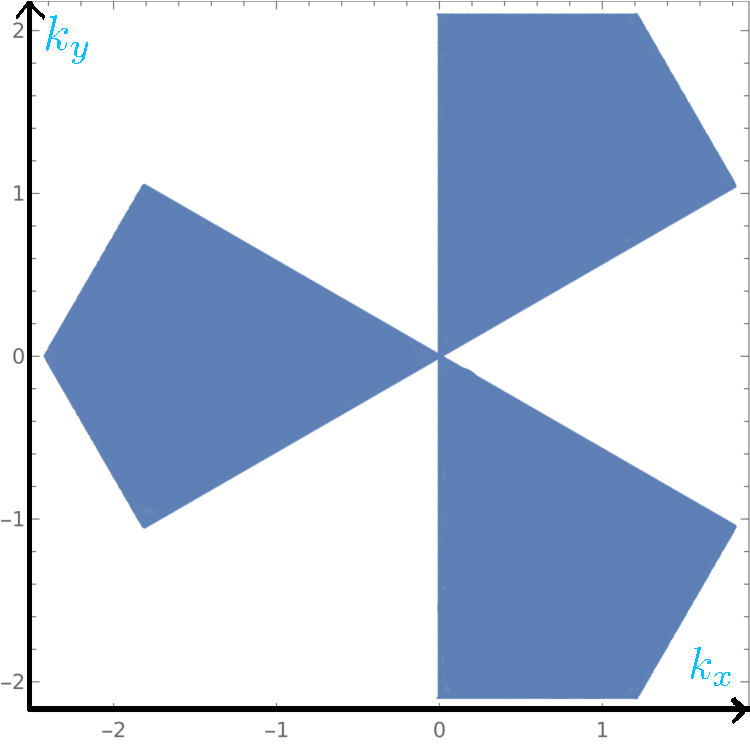
\includegraphics[width=0.31\linewidth]{fanBZ.pdf}}
	\caption{(a) The Brillouin Zone of a triangular lattice. (b) A single valley in the Brillouin Zone.
	}~\label{Fig:BZ}
\end{figure}
For simplicity, we can choose $t = -1$ in Eq. \eqref{Eq:GrapheneHopping} (in other words, we scale the whole Hamiltonian, and the parameter $m$ accordingly), and find the Chern Number for a single Valley in the Brillouin Zone. This can inded be experimentally achieved with cirlularly polarized electromagnetic waves \cite{valleyPolBilayerGraphene}. This calculation is done in Mathematica (code available at \cite{code:mathematicaCode}). 
Using the formula \eqref{Eq:BerryTwoBandFormula}, the Berry curvature for monolayer graphene only has a $z$ component, and it is,
$$\Omega_z = -\frac{3 \sqrt{3} m \sin \left(\frac{1}{2}(\sqrt{3} k_x -3 k_y)\right)}{4\left(4 \cos \left(\frac{\sqrt{3} k_x}{2}\right) \cos \left(\frac{3 k_y}{2}\right)+2 \cos (\sqrt{3} k_x)+m^{2}+3\right)^{3 / 2}}.$$
It is maximum at the $\vec{K}$, $\vec{K}'$ points.
We define a valley as the collection of points in the BZ, which are closer to one Dirac point than the other (see Fig. \ref{Fig:BZ}(b)).

In the numerical calculation, it was found that the valley Chern number is zero when the mass term $m = 0$, while $\mathcal{C} \rightarrow \mp \frac{1}{2}$ as $m \rightarrow 0^+$ and $0^-$. And, for the other valley, $\mathcal{C} \rightarrow \pm \frac{1}{2}$ as $m \rightarrow 0^+$ and $0^-$. For large values of $m$, the valley Chern number gradually decreases, and approaches $0$.

\begin{figure}[h!]
	\centering
	\subfigure[]{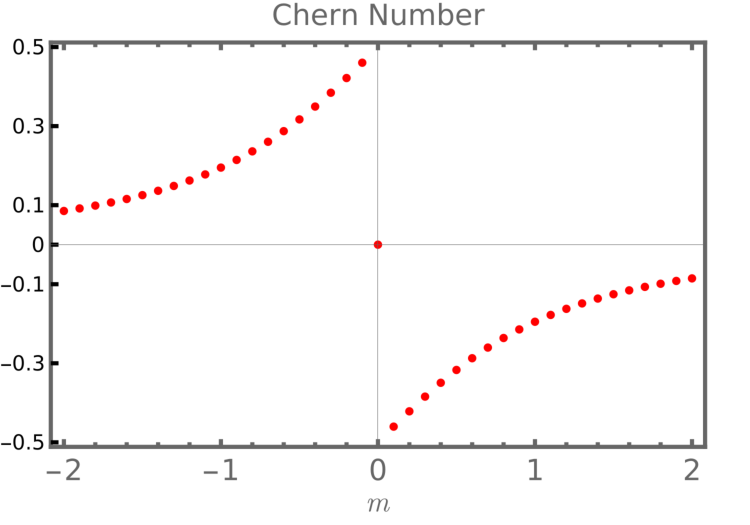
\includegraphics[width=0.46\linewidth]{chernnumber1.pdf}}
	\subfigure[]{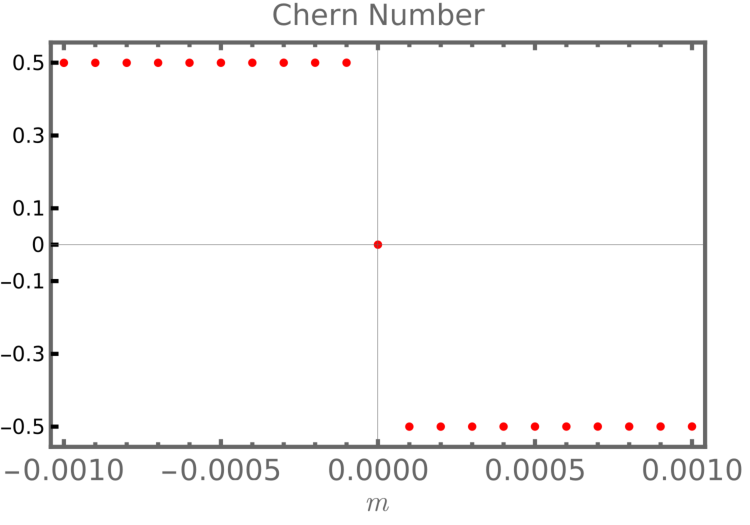
\includegraphics[width=0.46\linewidth]{chernZoom.pdf}}
	\caption{(a) Valley Chern Number as a function of $m$. (b) $\mathcal{C} \rightarrow \pm 0.5$ for very small, but non-zero values of $m$.
	}~\label{Fig:inner_products}
\end{figure}

This fractional value of valley Chern number is, again, not of any concern because we did not integrate over the whole Brillouin Zone.

Note the valley Chern number is $0$ exactly at $m= 0$, but it is $\pm \frac{1}{2}$ in the limit of $m \rightarrow 0^\mp$.

\section{Bilayer Graphene and Effective Two Band Hamiltonian}
In bilayer graphene, the electron can hop between the two layers, as well as within individual layers. Due to the interlayer hopping, the Dirac cones of the two layers would be hybridized.

We denote the localized Wannier functions as, $\ket{A,1} = (1,0,0,0)^T, \ket{A,2} = (0,1,0,0)^T, \ket{B,1} = (0,0,1,0)^T$ and $\ket{B,2} = (0,0,0,1)^T$, where $A,B$ stand for the the sublattice, and $1,2$ denote the layer index.
Here we use the model proposed by Zhang, MacDonald and Mele \cite{Zhang10546}, where the effective Hamiltonian near a Dirac Cone can be written as a sum of three terms,
$$ H = H_1 + H_{int} + H_2. $$
Here $H_1$ is the intra-layer hopping Hamiltonian of monolayer graphene, $H_1 = \nu q_{x} \sigma_{x} \tau_{0}+q_{y} \sigma_{y} \tau_{0}$, where $\nu = \pm 1$ depending on whether the Hamiltonian is describing the $\vec{K}$ or $\vec{K}'$ valley. The matrices $\sigma_{x,y,z}$ act on the $A, B$ degree of freedom, while the matrices $\tau_{x,y,z}$ act on the degree of freedom of the two layers.
$H_{int}$ is the inter-layer hopping Hamiltonian \footnote{\textit{int} stands for inter-layer, \textbf{not} interaction. The electrons are assumed to be non-interacting in this model.}.
When A site on the top layer hybridize with the A sites in the bottom layer, we can write,
$H_{int} = \frac{\gamma\left(\sigma_{x} \tau_{x}+\sigma_{y} \tau_{y}\right)}{2}$, with $\gamma$ being the hopping amplitude.
\begin{figure}[h!]
	\centering
	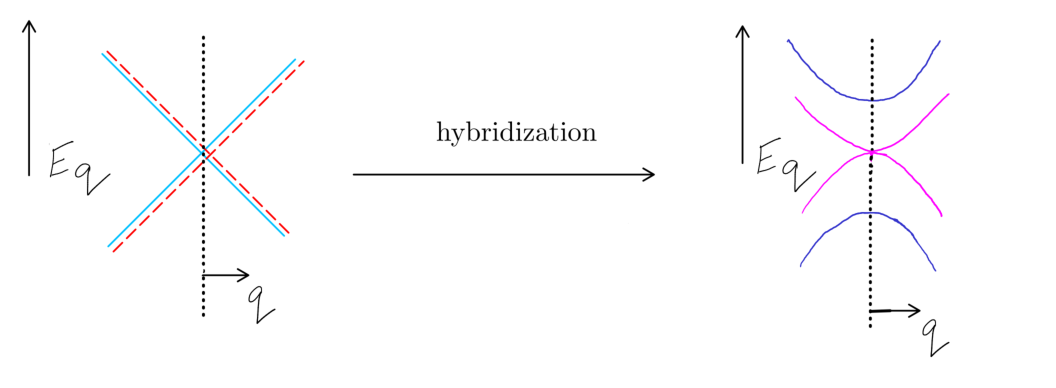
\includegraphics[width=0.7\linewidth]{hybridization.pdf}
	\caption{The Dirac cones of the two graphene layers (sky blue and red) are hybridized to form four bands. We want to calculate the effective Hamiltonian in the low energy subspace, comprising of the bands colored pink. It is found that the pink bands touch quadratically, when there is no external potential that breaks the symmetry between the two layers.}
	\label{fig:hybridization}
\end{figure}
We can also put an electric field perpendicular to the plane of the graphene sheets, and the two layers would have different potentials. This is modeled with the term, $H_2 = \Delta \sigma_0 \tau_z$. 
\subsection{Strategy for finding effective low energy Hamiltonian}
If we find the eigenvectors for a general value of $q_x$, $q_y$, and write the Hamiltonian in terms of them, the effective Hamiltonian would be diagonal in them, $H_{eff} = d_z \sigma_z$. But, the Berry curvature (Eq. \eqref{Eq:BerryTwoBandFormula}) is always zero for such a Hamiltonian. We have to fix a value of ($q_x$, $q_y$), find a low energy basis, and then find the effective Hamiltonian in this basis.
To find the effective low energy subspace, we consider $H_0$ as a perturbation (notice that $H_0 = 0$ at $q_x = q_y =0$.) Let us put $\gamma = 1$ for simplicity (i.e., we scale all other quantities with $\gamma$.)

Then, $H_{int} = \begin{pmatrix}
	0 & 0 & 0 & 0 \\
	0 & 0 & 1 & 0 \\
	0 & 1 & 0 & 0 \\
	0 & 0 & 0 & 0 
\end{pmatrix}$, and $ H_{int} + H_2 = \begin{pmatrix}
	\Delta & 0 & 0 & 0 \\
	0 & -\Delta & 1 & 0 \\
	0 & 1 & \Delta & 0 \\
	0 & 0 & 0 & -\Delta 
\end{pmatrix} $.

The eigenvectors of $H_{int}$ are, $\underbrace{\ket{\phi_1}}_{E = 0} = (1,0,0,0)^T$, $\underbrace{\ket{\phi_2}}_{E = 0} = (0,0,0,1)^T$,
$\underbrace{\ket{\phi_3}}_{E = 1} = \frac{1}{\sqrt{2}}(0,1,1,0)^T$,
$\underbrace{\ket{\phi_4}}_{E = -1} = \frac{1}{\sqrt{2}}(0,1,-1,0)^T$.

Let $P = \ket{\phi_1}\bra{\phi_1} + \ket{\phi_2}\bra{\phi_2}$, the projector in the low energy subspace, and $Q = 1 - P = \ket{\phi_3}\bra{\phi_3} + \ket{\phi_4}\bra{\phi_4}$, the projector in the high energy subspace.
Then, the effective form of $H_1$ in the low energy subspace would be, using the standard formula of degenerate perturbation theory,
$$H_{1,2} = P H_{int} P + P H_1 Q \frac{1}{P H_{int} P - Q H_{int} Q} Q H_1 P .$$
Since $P H_{int} P$ is already 0, we have, $H_{1,2} =- P H_1 Q \frac{1}{H_{int}} Q H_1 P$. With all the quantities already defined, this calculation is straightforward to do, and we get (see Appendix \ref{app:EffHamiltonian} for details), $H_{1,2} = \begin{pmatrix}
	0 & -(\nu q_x - i q_y)^2\\
	-(\nu q_x + i q_y)^2 & 0
\end{pmatrix} = -(q_x^2 - q_y^2) \tilde{\sigma}_x - 2 \nu q_x q_y \tilde{\sigma}_y$.


$\ket{\phi_1}$ and $\ket{\phi_2}$, defined above, are also eigenvectors of $H_2$, with eigenvalues $\Delta$ and $-\Delta$, respectively.

$$ (H_2)_{\ket{\phi_1}, \ket{\phi_2}} = \begin{pmatrix}
	\Delta & 0 \\
	0 & -\Delta
\end{pmatrix} = \Delta \tilde{\sigma}_z
$$
Since this term is already diagonal, we don't need to do calculate second order perturbation of this term.

Then the effective Hamiltonian in the low energy subspace is,
\begin{equation}\label{Eq:EffectiveLowEnergyTwoBandHamiltonian}
	\left(H_{eff}\right)_{\ket{\phi_1}, \ket{\phi_2}} = -(q_x^2 - q_y^2) \tilde{\sigma}_x - 2 \nu q_x q_y \tilde{\sigma}_y + \Delta \tilde{\sigma}_z 
\end{equation}
With this effective Hamiltonian \footnote{Note that when the external potential $\Delta = 0$, the dispersion relation is, $\vec{E}_q = \pm (q_x^2 + q_y^2)$, i.e. the \textit{bands touch \textbf{quadratically}}. However, in this model, when the bands touch, the Berry curvature becomes 0 (so does the Chern number). However, in the limit of even infinitesimally small external potential, there is a non-zero Chern number of magnitude 1.}, we can employ the formula in Eq. \eqref{Eq:BerryTwoBandFormula}, and find, $\boxed{\vec{\Omega}(\vec{q}) = \frac{2 \nu \Delta (q_x^2 + q_y^2)}{((q_x^2 + q_y^2)^2 + \Delta^2)^{\frac{3}{2}}}    \hat{z}}$.
Its integral over the whole BZ is 0, because the two valleys $\vec{K}$ and $\vec{K}'$ have opposite signs of $\nu$. This is expected, because the model has time reversal symmetry, and the overall band Chern number is 0.


However, if we can selectively fill one of the valleys (this can be done with circularly polarized light), then we can get a non-zero anomalous Hall response. The Berry curvature falls off very quickly as a function of $q$, and to estimate the Chern number of a single valley, we can integrate from $q = 0$ to $\infty$.

The Chern number of a single valley is then, $\boxed{\mathcal{C}_{\nu} \approx \frac{1}{2\pi} \int_0^{\infty} \frac{2 \nu \Delta q^2}{(q^4 + \Delta^2)^{\frac{3}{2}}} 2 \pi q dq = \text{sign}(\Delta) \nu = \pm 1}$.

\section{A class of models with non-linear band touching and non-zero Berry curvature}

Consider the general class of models with a Hamiltonian,
$H(\vec{k}) = k_x \sigma_x + k_y \sigma_y + \alpha (k_x^2 + k_y^2)^n \sigma_z$. The dispersion is a Dirac-like cone, where the mass can depend on the momentum, and the mass is zero at zero momentum.
The dispersion relation is, $\varepsilon_k = \pm \sqrt{k^2 + \alpha^2 k^{4n}}$. For $n > \frac{1}{2}$, while the band is linear near $k = 0$, it becomes curved for large momenta. While for $0<n<\frac{1}{2}$, the band is non-linear near the origin, while it is almost linear for large momenta.

Using the formula Eq. \eqref{Eq:BerryTwoBandFormula}, the Berry curvature of the ground state is found to be,

$$\Omega_z = \frac{\alpha (1 - 2n) k^{2n}}{2(k^2 + \alpha^2 k^{4n})^{\frac{3}{2}}}.$$
For this model, the valley Chern number is, $\mathcal{C} = +0.5$ for $0<n<0.5$, and $\mathcal{C} = -0.5$ for $n>0.5$.
\section{Fractional Chern Numbers?}
\subsection{Argument why Chern number should be an integer when Berry curvature is integrated over the first Brillouin Zone}\label{sebsec:integer-chern-argument}

\begin{figure}[h!]
	\centering
	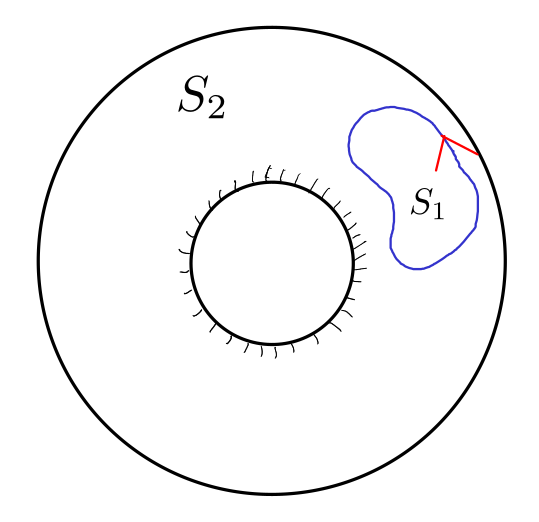
\includegraphics[width=0.3\linewidth]{torus}
	\caption{The Brillouin Zone can be mapped to a Torus.}
	\label{fig:torus}
\end{figure}
The Brillouin Zone is periodic in $k_x$ and $k_y$, and can be mapped to a torus. Suppose a Bloch wavepacket moves along the blue curve, and returns to its initial position (see Fig. \ref{fig:torus}). Then, the geometric phase acquired by the electron would be, $\oint \vec{A}(\vec{k})\cdot d\vec{k}$. Using Stokes' theorem, we can rewrite this as, $\int_{S_1} \nabla \times \vec{A}(\vec{k}) d^2 k$ , and the phase factor is, $e^{i\int_{S_1} \nabla \times \vec{A}(\vec{k}) d^2 k}$. But, we could apply Stokes' theorem on the other surface, $S_2$, and rewrite the phase factor as, $e^{-i\int_{S_2} \nabla \times \vec{A}(\vec{k}) d^2 k}$. The negative sign appears due to the opposite orientation.
However, since the overall phase factor has to be unique (because it can be found with interference experiments), we must have, $e^{i\int_{S_1} \nabla \times \vec{A}(\vec{k}) d^2 k} = e^{-i\int_{S_2} \nabla \times \vec{A}(\vec{k}) d^2 k}$, which implies, $e^{i\int_{B Z} \nabla \times \vec{A}(\vec{k}) d^2 k} = 1$.

Then, we must have, $\int_{B Z} \nabla \times \vec{A}(\vec{k}) d^2 k = 2 n \pi$, with $n \in \mathbb{Z}$, implying that the Chern number $\mathcal{C}=\frac{1}{2\pi} \int_{B Z} \nabla \times \vec{A}(\vec{k}) d^2 k$ is an integer.

\subsection{Possible explanation for half-integer Chern numbers}
We see half integer Chern numbers when there is a band gap closing, which causes $\vec{\Omega}$ to diverge at the point of band gap closing. Our argument in the previous section does not anymore hold because we cannot apply the result of Stokes' theorem, as $\vec{\Omega}$ is not well defined at all points on the Brillouin Zone.

And when the we consider a continuum model, with a infinite range of momentum, it is not a closed surface, and here the half integer Chern number is not an issue. 


\chapter{Results}
In this thesis, the full expressions of electric and energy current densities are worked out up to linear order in externally applied fields (electric field, chemical potential gradient and temperature gradient) when there is a non-zero Berry curvature and a non-zero external magnetic field. All the missing steps in existing research papers are worked out in details.

It was verified that in the linear regime, the anomalous Hall and the anomalous Nernst effects are caused by the equilibrium part of the electronic distribution (the Fermi distribution), whereas the regular Ohmic transport, the regular Hall effect, and the regular Nernst effects are caused by the non-equilibrium part of the distribution. The Einstein relation and the Onsager relations are verified separately for the contributions from the equilibrium and the non-equilibrium parts of the distribution, so that they would also hold for the overall transport.

The Einstein and the Onsager relations only hold for the transport currents, which is obtained by subtracting the circulating magnetization currents from the total current. It was found that for the Einstein relation to hold, the energy magnetization has to satisfy a condition, which was not pointed out in existing literature up to the best knowledge of the author.

For a 2D system with a non-zero Berry curvature in reciprocal space, and there is a non-zero magnetic field, the full non-equilibrium part of the distribution was analytically calculated up to linear order in the external fields, by treating the magnetic field as a perturbation in the Boltzmann transport equation. This distribution function (Eq. \eqref{Eq:g_non_zero_chem_temp_grad}) can be used to quantitatively compute the Ohmic conductivity, the Hall and the Nernst response, the Seebeck and Peltier coefficients, and other transport properties. I could not find this expression of the non-equilibrium distribution (when both the non-zero magnetic field and Berry curvature are non-zero) in existing literature.

In the later part of the thesis, some microscopic models with non-zero Berry curvatures were explored and their Chern numbers were calculated. It was found that a linear band touching cannot give rise to a non-zero Berry curvature. To get a non-zero Berry curvature and a non-zero valley Chern number, we either need a band gap (in other words a massive Dirac cone), or the bands must touch non-linearly (i.e. there must be a curvature in the dispersion). A microscopic model was proposed where the bands touch non-linearly and it has a non-zero Berry curvature, leading to a finite Chern number.

A detailed derivation of the effective two band Hamiltonian (Eq. \eqref{Eq:EffectiveLowEnergyTwoBandHamiltonian}) near the Dirac cones of bilayer graphene was provided. It was calculated from an effective four-band Hamiltonian. The procedure of this calculation was not outlined in existing literature. It was found that in order to find the correct form of the effective Hamiltonian and Berry curvature, one needs to go to the center of the valley and fix the momentum in the Hamiltonian, and work with its eigenbasis, treating the change in momentum from that point as a perturbation. Instead, if one takes the eigenbasis of the total four band Hamiltonian at arbitrary momenta, and considers the effective Hamiltonian as the low energy subspace of that, the resulting effective Hamiltonian would always be diagonal (because it is written in the eigenbasis) and the Berry curvature obtained from the resulting effective two band Hamiltonian would be identically zero. This is because in that case, one is also rotating one's coordinate axes when going to a new momentum eigenbasis. But to calculate Berry curvature, first one needs to fix the coordinate axes of the crystal momenta, and this is the method to correctly obtain the Berry curvature.

\chapter*{\center Appendices}%
\addcontentsline{toc}{chapter}{\numberline{}Appendices}%
\appendix

\chapter{Calculation of expectation value of the position of the wavepacket}~\label{app:center-at-zero-time}
We want to build a wavepacket centered about $\vec{r}= \vec{r}_0, \vec{k}= \vec{k}_0$. The calculation of this appendix is loosely based on Ref. \cite{ralph2020berry}.


Let  $w(\vec{k} - \vec{k}_0)$ be a real weight function, sharply peaked at $\vec{k}_0$. If we take a wavepacket of the form $\int d\vec{k} w(\vec{k} - \vec{k}_0) e^{-i \vec{k} \cdot \vec{r}_0 } \left(e^{i \vec{k} \cdot\vec{r}} u_{n,\vec{k}}(\vec{r})\right)$, it may not be sharply peaked at $\vec{r} = \vec{r}_0$, because, although the functions $e^{i \vec{k} \cdot(\vec{r} - \vec{r}_0)}$ interfere constructively about $\vec{r} = \vec{r}_0$, the functions $u_{n,\vec{k}}(\vec{r}_0)$ may have different phases for different values of $\vec{k}$. To take account of this, let us consider the wavefunction, 
\begin{equation}\label{Eq:wavefunction-X}
	\phi_{\vec{X}}(\vec{r}, t=0) = \int d\vec{k} w(\vec{k} - \vec{k}_0) e^{i \vec{X}(\vec{k_0})\cdot (\vec{k} - \vec{k}_0)} e^{-i \vec{k} \cdot \vec{r}_0 } \left(e^{i \vec{k} \cdot\vec{r}} u_{n,\vec{k}}(\vec{r})\right)
\end{equation}

\section{Normalization}\label{app:sec:Bloch-normalization}
 Let us choose the normalization of the individual Bloch wavefunctions such that

\begin{equation}\label{Eq:BlochNormalization}
	\int_{\text{unit cell}} d\vec{r} |u_{n,\vec{k}}(\vec{r})|^2 = 1
\end{equation}

Then, $\bra{\phi_{\vec{X}}(\vec{r}, t=0)}\ket{\phi_{\vec{X}}(\vec{r}, t=0)}$
$$ = \int_{\text{all space}} d\vec{r} \int \int d\vec{k}_2 d\vec{k}_1  w(\vec{k}_1 - \vec{k}_0) w(\vec{k}_2 - \vec{k}_0) e^{i \vec{X}(\vec{k_0})\cdot (\vec{k}_1 - \vec{k}_2)} e^{i (\vec{k}_1 - \vec{k}_2) \cdot (\vec{r} - \vec{r}_0) }  u^*_{n,\vec{k}_2}(\vec{r}) u_{n,\vec{k}_1}(\vec{r})$$

Let us perform the $\vec{r}$ integral first. We can utilize the periodicity of $u_{n,\vec{k}_1}$ and rewrite, 
$$\int_{\text{all space}} d\vec{r} e^{i (\vec{k}_1 - \vec{k}_2) \cdot (\vec{r} - \vec{r}_0) }  u^*_{n,\vec{k}_2}(\vec{r}) u_{n,\vec{k}_1}(\vec{r})$$
$$ =  \sum_{ \vec{R}}  e^{i (\vec{k}_1 - \vec{k}_2)\cdot \vec{R} } \int_{\text{unit cell}} d\vec{r} e^{i (\vec{k}_1 - \vec{k}_2) \cdot (\vec{r} - \vec{r}_0) }  u^*_{n,\vec{k}_2}(\vec{r}) u_{n,\vec{k}_1}(\vec{r}) $$
where the index $\vec{R}$ runs over the coordinates of the unit cells, and the integral is over a single unit cell (and it is the same for every unit cell). The sum is zero unless $\vec{k}_1 - \vec{k}_2$ is a reciprocal lattice vector (because otherwise, the phase factors $e^{i (\vec{k}_1 - \vec{k}_2)\cdot \vec{R} }$ would all cancel each other). Since both $\vec{k}_1$ and $\vec{k}_2$ belong to the first Brillouin zone, we must have $\vec{k}_1 = \vec{k}_2$.  For a finite system with $N$ unit cells, $\vec{k}$ can only take discrete values, and the sum is $N \delta_{\vec{k}_1,\vec{k}_2}$. When $N$ is large, the points in reciprocal space are dense, and we can approximate, $\sum_{ \vec{R}}  e^{i (\vec{k}_1 - \vec{k}_2)\cdot \vec{R} } \rightarrow \frac{1}{V_c} \int d \vec{r} e^{i (\vec{k}_1 - \vec{k}_2)\cdot \vec{r} } = \frac{(2 \pi)^d}{V_c} \delta (\vec{k}_1 - \vec{k}_2)$, where $V_c$ is the volume of the $d$ dimensional unit cell. We can further write $\frac{(2 \pi)^d}{V_c} = V_{\text{BZ}}$, where $V_{\text{BZ}}$ is the volume of the Brillouin zone.

Also, when $\vec{k}_1 = \vec{k}_2$, the periodic part of the sum, $\int_{\text{unit cell}} d\vec{r} e^{i (\vec{k}_1 - \vec{k}_2) \cdot (\vec{r} - \vec{r}_0) }  u^*_{n,\vec{k}_2}(\vec{r}) u_{n,\vec{k}_1}(\vec{r}) = 1$, due to normalization of Bloch wavefunctions (Eq. \eqref{Eq:BlochNormalization}). Finally, we get,
$$\int_{\text{all space}} d\vec{r} e^{i (\vec{k}_1 - \vec{k}_2) \cdot (\vec{r} - \vec{r}_0) }  u^*_{n,\vec{k}_2}(\vec{r}) u_{n,\vec{k}_1}(\vec{r}) = V_{\text{BZ}} \delta (\vec{k}_1 - \vec{k}_2) $$

Then, $\bra{\phi_{\vec{X}}(\vec{r}, t=0)}\ket{\phi_{\vec{X}}(\vec{r}, t=0)}$
$$ =  V_{\text{BZ}} \int \int d\vec{k}_2 d\vec{k}_1   \delta (\vec{k}_1 - \vec{k}_2) w(\vec{k}_1 - \vec{k}_0) w(\vec{k}_2 - \vec{k}_0) e^{i \vec{X}(\vec{k_0})\cdot (\vec{k}_1 - \vec{k}_2)} = V_{\text{BZ}} \int d\vec{k} [w(\vec{k} - \vec{k}_0)]^2$$

Then, have to scale $w(\vec{k} - \vec{k}_0)$ such that 
\begin{equation}\label{Eq:WavepacketNormalization}
	\int d\vec{k} [w(\vec{k} - \vec{k}_0)]^2 = \frac{1}{V_\text{BZ}}
\end{equation}


\section{Calculation of $\expval{\vec{r}}$}\label{app:calculation-of-<r>}

\textbf{Result}: For this wavefunction,
\begin{equation}\label{Eq:app:expectation-value-of-r}
\expval{\vec{r}}_{\phi_{\vec{X}}} = \bra{\phi_X(t=0)} \vec{r} \ket{\phi_X(t=0)} = \vec{r}_0 - \vec{X}(\vec{k}_0) + \vec{A}(\vec{k}_0)
\end{equation}
where  $\vec{A}(\vec{k}_0)$ is the Berry connection.

\textbf{Proof}: For convenience, let us calculate $\bra{\phi_X(\vec{r}, t=0)} \vec{r} - \vec{r}_0 \ket{\phi_X(\vec{r}, t=0)}$
 $$ = \int \int d\vec{k}_1 d\vec{k}_2 w(\vec{k}_2 - \vec{k}_0) w(\vec{k}_1 - \vec{k}_0) e^{-i \vec{X}(\vec{k}_0)\cdot (\vec{k}_2 - \vec{k}_0)} e^{-i \vec{k}_2 \cdot (\vec{r} - \vec{r}_0)} u^*_{n,\vec{k}_2}(\vec{r}) (\vec{r} - \vec{r}_0)e^{i \vec{X}(\vec{k}_0)\cdot (\vec{k}_1 - \vec{k}_0)} e^{i \vec{k}_1 \cdot (\vec{r} - \vec{r}_0)} u_{n,\vec{k}_1}(\vec{r})$$
 
 Let us rewrite, $(\vec{r} - \vec{r}_0)e^{i \vec{k}_1 \cdot (\vec{r} - \vec{r}_0)} = \frac{1}{i} \nabla_{_{\vec{k}_1}} e^{i \vec{k}_1 \cdot (\vec{r} - \vec{r}_0)}$.
 
 Then, $w(\vec{k}_1 - \vec{k}_0) (\vec{r} - \vec{r}_0)e^{i \vec{X}(\vec{k}_0)\cdot (\vec{k}_1 - \vec{k}_0)} e^{i \vec{k}_1 \cdot (\vec{r} - \vec{r}_0)} u_{n,\vec{k}_1}(\vec{r})$
 $$ = \frac{1}{i} \left[\nabla_{_{\vec{k}_1}} e^{i \vec{k}_1 \cdot (\vec{r} - \vec{r}_0)}\right] w(\vec{k}_1 - \vec{k}_0) e^{i \vec{X}(\vec{k}_0)\cdot (\vec{k}_1 - \vec{k}_0)}  u_{n,\vec{k}_1}(\vec{r})$$
 $$ = \frac{1}{i} \nabla_{_{\vec{k}_1}} \left[ e^{i \vec{k}_1 \cdot (\vec{r} - \vec{r}_0)} w(\vec{k}_1 - \vec{k}_0) e^{i \vec{X}(\vec{k}_0)\cdot (\vec{k}_1 - \vec{k}_0)}  u_{n,\vec{k}_1}(\vec{r})\right] - \frac{1}{i}  e^{i \vec{k}_1 \cdot (\vec{r} - \vec{r}_0)} \nabla_{_{\vec{k}_1}} \left[w(\vec{k}_1 - \vec{k}_0) e^{i \vec{X}(\vec{k}_0)\cdot (\vec{k}_1 - \vec{k}_0)}  u_{n,\vec{k}_1}(\vec{r})\right]. $$
 
 The first term would be zero when integrated over $\vec{k}_1$, because the sharply peaked weight $w(\vec{k}_1 - \vec{k}_0) \rightarrow 0$, far away from $\vec{k}_0$. Let us then look at the second term, $- \frac{1}{i}  e^{i \vec{k}_1 \cdot (\vec{r} - \vec{r}_0)} \nabla_{_{\vec{k}_1}} \left[w(\vec{k}_1 - \vec{k}_0) e^{i \vec{X}(\vec{k}_0)\cdot (\vec{k}_1 - \vec{k}_0)}  u_{n,\vec{k}_1}(\vec{r})\right]$
 $$ = - \frac{1}{i}  e^{i \vec{k}_1 \cdot (\vec{r} - \vec{r}_0)} e^{i \vec{X}(\vec{k}_0)\cdot (\vec{k}_1 - \vec{k}_0)} \left[ \nabla_{_{\vec{k}_1}} w(\vec{k}_1 - \vec{k}_0)  u_{n,\vec{k}_1}(\vec{r}) +  w(\vec{k}_1 - \vec{k}_0)  \nabla_{_{\vec{k}_1}} u_{n,\vec{k}_1}(\vec{r}) + i \vec{X}(\vec{k}_0) w(\vec{k}_1 - \vec{k}_0) u_{n,\vec{k}_1}(\vec{r}) \right]$$
 
 Let us first take the first of the three terms in the third bracket, and calculate its contribution to $\expval{\vec{r} - \vec{r}_0}_{\phi_{\vec{X}}}$, which we denote as $\expval{\vec{r} - \vec{r}_0}_1$
 $$= - \int_{\vec{r}} \int_{\vec{k}_1} \int_{\vec{k}_2} w(\vec{k}_2 - \vec{k}_0) e^{-i \vec{X}(\vec{k}_0)\cdot (\vec{k}_2 - \vec{k}_0)} e^{-i \vec{k}_2 \cdot (\vec{r} - \vec{r}_0)} u^*_{n,\vec{k}_2}(\vec{r}) \left[e^{i \vec{X}(\vec{k}_0)\cdot (\vec{k}_1 - \vec{k}_0)} e^{i \vec{k}_1 \cdot (\vec{r} - \vec{r}_0)} \nabla_{_{\vec{k}_1}} w(\vec{k}_1 - \vec{k}_0) u_{n,\vec{k}_1}(\vec{r})\right]$$
 Now, when we integrate over $\vec{r}$, we would get a factor of $\delta(\vec{k}_1 - \vec{k}_2)$, which would force $k_1 = k_2$.
 Then, we would get a factor, $\int d\vec{k} w(\vec{k} - \vec{k}_0) \nabla_{_{\vec{k}}} w(\vec{k} - \vec{k}_0)$. The first term being sharply peaked at $\vec{k}_0$ would pick out the second term at $\vec{k}_0 = \vec{k}$. But  $\nabla_{_{\vec{k}}} w(\vec{k} - \vec{k}_0) |_(\vec{k} - \vec{k}_0) = 0$, as $\vec{k}_0$ is a maxima of   $w(\vec{k} - \vec{k}_0)$. As a result, this term is 0.
 
 Now consider the second term,$ \expval{\vec{r} - \vec{r}_0}_2$
 $$ = - \frac{1}{i} \int_{\vec{r}} \int_{\vec{k}_1} \int_{\vec{k}_2}  w(\vec{k}_2 - \vec{k}_0) e^{-i \vec{X}(\vec{k}_0)\cdot (\vec{k}_2 - \vec{k}_0)} e^{-i \vec{k}_2 \cdot (\vec{r} - \vec{r}_0)} u^*_{n,\vec{k}_2}(\vec{r}) \left[e^{i \vec{X}(\vec{k}_0)\cdot (\vec{k}_1 - \vec{k}_0)} e^{i \vec{k}_1 \cdot (\vec{r} - \vec{r}_0)}  w(\vec{k}_1 - \vec{k}_0) \nabla_{_{\vec{k}_1}} u_{n,\vec{k}_1}(\vec{r})\right]$$
 When we integrate over $\vec{r}$, we get, 
 $$\int_{\text{all space}} d\vec{r} e^{i (\vec{k}_1 - \vec{k}_2) \cdot (\vec{r} - \vec{r}_0) }  u^*_{n,\vec{k}_2}(\vec{r}) \nabla_{_{\vec{k}_1}} u_{n,\vec{k}_1}(\vec{r})$$
 $$ =  \sum_{ \vec{R}}  e^{i (\vec{k}_1 - \vec{k}_2)\cdot \vec{R} } \int_{\text{unit cell}} d\vec{r} e^{i (\vec{k}_1 - \vec{k}_2) \cdot (\vec{r} - \vec{r}_0) }  u^*_{n,\vec{k}_2}(\vec{r}) \nabla_{_{\vec{k}_1}} u_{n,\vec{k}_1}(\vec{r}) $$
 $$ = V_\text{BZ} \delta(\vec{k}_1 - \vec{k}_2) \int_{\text{unit cell}} d\vec{r} e^{i (\vec{k}_1 - \vec{k}_2) \cdot (\vec{r} - \vec{r}_0) }  u^*_{n,\vec{k}_2}(\vec{r}) \nabla_{_{\vec{k}_1}} u_{n,\vec{k}_1}(\vec{r})$$
 $$ = V_\text{BZ} \delta(\vec{k}_1 - \vec{k}_2) \int_{\text{unit cell}} d\vec{r}  u^*_{n,\vec{k}_1}(\vec{r}) \nabla_{_{\vec{k}_1}} u_{n,\vec{k}_1}(\vec{r})$$
 $$ = V_\text{BZ} \delta(\vec{k}_1 - \vec{k}_2) \frac{1}{i} \vec{A}(\vec{k}_1)$$
 
 Putting this back in the expression of $\expval{\vec{r} - \vec{r}_0}_2$, and carrying out the integral over the delta function, we get,
 $$\expval{\vec{r} - \vec{r}_0}_2 = -\frac{1}{i}\int_{\vec{k}_1} [w(\vec{k}_1 - \vec{k}_0)]^2 \frac{1}{i} \vec{A}(\vec{k}_1) V_\text{BZ} \approx \vec{A}(\vec{k}_0) \int_{\vec{k}_1} [w(\vec{k}_1 - \vec{k}_0)]^2 V_\text{BZ} = \vec{A}(\vec{k}_0),$$ using the normalization condition in Eq. \eqref{Eq:WavepacketNormalization}.
 
 Let us know take the final term inside the third bracket, $i \vec{X}(\vec{k}_0) w(\vec{k}_1 - \vec{k}_0) u_{n,\vec{k}_1}(\vec{r})$. Its contribution to $\expval{\vec{r} - \vec{r}_0}$ is, $ \expval{\vec{r} - \vec{r}_0}_3$
 $$ = -\frac{1}{i} \int_{\vec{r}} \int_{\vec{k}_1} \int_{\vec{k}_2} w(\vec{k}_2 - \vec{k}_0) e^{-i \vec{X}(\vec{k}_0)\cdot (\vec{k}_2 - \vec{k}_0)} e^{-i \vec{k}_2 \cdot (\vec{r} - \vec{r}_0)} u^*_{n,\vec{k}_2}(\vec{r}) \left[e^{i \vec{X}(\vec{k}_0)\cdot (\vec{k}_1 - \vec{k}_0)} e^{i \vec{k}_1 \cdot (\vec{r} - \vec{r}_0)} i \vec{X}(\vec{k}_0) w(\vec{k}_1 - \vec{k}_0) u_{n,\vec{k}_1}(\vec{r})\right]$$
 $$= -\vec{X}(\vec{k}_0) \bra{\phi_{\vec{X}}(t=0)}\ket{\phi_{\vec{X}}(t=0)} = -\vec{X}(\vec{k}_0)$$
 
 Adding all the non-zero terms, we get,
$ \expval{\vec{r} - \vec{r}_0}_{\phi_{\vec{X}}} = \vec{A}(\vec{k}_0) -\vec{X}(\vec{k}_0) $, from which Eq. \eqref{Eq:app:expectation-value-of-r} follows.

\section{Wavepacket centered at $\vec{r}_0$}
We found that the wavepacket in Eq. \eqref{Eq:wavefunction-X} is centered at $\vec{r}_0 - \vec{X(\vec{k}_0)} + \vec{A(\vec{k}_0)}$. Then, to get a wavepacket centered at $\vec{r}_0$, we need to choose $\vec{X} = \vec{A}$, and the desired wavefunction is,
\begin{equation}\label{Eq:wavefunction-r0}
	\phi_{\vec{X}}(\vec{r}, t=0) = \int d\vec{k} w(\vec{k} - \vec{k}_0) e^{i \vec{A}(\vec{k_0})\cdot (\vec{k} - \vec{k}_0)} e^{-i \vec{k} \cdot \vec{r}_0 } \left(e^{i \vec{k} \cdot\vec{r}} u_{n,\vec{k}}(\vec{r})\right)
\end{equation}
\section{Calculation of the center of the time evolved wavepacket}~\label{app:center-at-new-time}
Recall the the state $e^{i \vec{k}\cdot\vec{r}} u_{\vec{k}}(\vec{r})$ evolves as, $e^{i {\vec{k + \Delta\vec{{k}}}\cdot\vec{r}}} e^{i \vec{A}(\vec{k})\cdot \Delta{\vec{k}}} e^{- \frac{i\varepsilon_{_{\vec{k}}} \Delta t}{\hbar}}u_{\vec{k}+\Delta\vec{ k}}(\vec{r})$. Then the wavefunction of the wavepacket is,
$$
	\psi(\vec{r}, \Delta t) = \int d\vec{k} w(\vec{k} - \vec{k}_0) e^{i \vec{A}(\vec{k_0})\cdot (\vec{k} - \vec{k}_0)} e^{-i \vec{k} \cdot \vec{r}_0 } \left(e^{i (\vec{k} + \Delta\vec{k})\cdot\vec{r}} e^{i \vec{A}(\vec{k})\cdot \vec{\Delta{k}}} e^{-i \frac{\varepsilon_{_{\vec{k}}} \Delta t}{\hbar}} u_{n, \vec{k}+\Delta \vec{k}} \right).$$
	Let $\vec{k} + \Delta \vec{k} = \vec{k}'$. Note that up to linear order in $\Delta t$, $\Delta \vec{k} = \Delta \vec{k}'$. Then, after changing variables in the integral,
	$$
	\begin{aligned}\psi(\vec{r}, \Delta t) &= \int d\vec{k}' w(\vec{k}' - \Delta\vec{k} - \vec{k}_0) e^{i \vec{A}(\vec{k_0})\cdot (\vec{k}' - \Delta \vec{k} - \vec{k}_0)} e^{-i (\vec{k}' - \Delta \vec{k})  \cdot \vec{r}_0 } \left(e^{i \vec{k}'\cdot\vec{r}} e^{i \vec{A}(\vec{k}'-\Delta\vec{k})\cdot \Delta\vec{k}} e^{-i \frac{\varepsilon_{_{\vec{k}}} \Delta t}{\hbar}} u_{n, \vec{k}'} \right)
	\\
	&= e^{i \left(\Delta \vec{k}_0 \cdot \vec{r}_0 - \frac{\varepsilon_{_{\vec{k}}} \Delta t}{\hbar}\right)} \int d\vec{k}' w(\vec{k}' - \Delta\vec{k} - \vec{k}_0) e^{i \vec{A}(\vec{k_0})\cdot (\vec{k}' - \vec{k}_0)} e^{i \vec{k}'\cdot(\vec{r} - \vec{r}_0)} e^{i \left[\vec{A}(\vec{k}'-\Delta\vec{k}) - \vec{A}(\vec{k}_0)\right]\cdot \Delta\vec{k}} e^{-i \frac{\nabla \varepsilon_{_{\vec{k}} \cdot (\vec{k}' - \vec{k}_0)}}{\hbar}} u_{n, \vec{k}'} 
\end{aligned}
$$
The weight function will force $\Delta \vec{k} = \left. \Delta \vec{k} \right|_{\vec{k} = \vec{k}_0} \equiv \Delta \vec{k}_0$.
We first simplify, $\vec{A}(\vec{k}' - \Delta \vec{k}) - \vec{A}(\vec{k}_0) = \left((\vec{k}' - \Delta \vec{k} - \vec{k}_0) \cdot \nabla_{\vec{k}} \right) \vec{A}(\vec{k}_0)$.
Then, 
$$
\begin{aligned}
	\Delta \vec{k}_0 \cdot [\vec{A}(\vec{k}' - \Delta \vec{k}') - \vec{A}(\vec{k}_0)] &= \Delta \vec{k}_0 \cdot [\left((\vec{k}' - \Delta \vec{k} - \vec{k}_0) \cdot \nabla_{\vec{k}} \right) \vec{A}(\vec{k}_0)] \\
	& = \Delta {\vec{k}_0}_\mu (\vec{k}' - \Delta \vec{k} - \vec{k}_0)_\nu \partial_\nu \vec{A}_\mu (\vec{k}_0) \\
	& = (\vec{k}' - \Delta \vec{k} - \vec{k}_0) \left. \cdot \nabla_{\vec{k}} \left(\vec{A}(\vec{k}) \cdot \Delta \vec{k}_0 \right) \right|_{\vec{k} = \vec{k}_0}
\end{aligned}$$
Using the result from Eq. \eqref{Eq:app:expectation-value-of-r},
$$
\begin{aligned}
\expval{\vec{r} - \vec{r}_0}(t=\Delta t) &= \vec{A}(\vec{k}_0 + \Delta \vec{k}_0) - \vec{A}(\vec{k}_0) - \nabla_{\vec{k}_0}(\vec{A}(\vec{k}_0)\cdot \Delta \vec{k}_0) + \frac{1}{\hbar} \nabla_{_{\vec{k}_0}} \varepsilon_{_{\vec{k}_0}} \Delta t \\
&= (\Delta \vec{k}_0 \cdot \nabla) \vec{A}(\vec{k}_0) - \nabla_{\vec{k}_0}(\vec{A}(\vec{k}_0)\cdot \Delta \vec{k}_0) + \frac{1}{\hbar} \nabla_{_{\vec{k}_0}} \varepsilon_{_{\vec{k}_0}} \Delta t \\
&= -\Delta \vec{k}_0 \times (\nabla \times \vec{A}(\vec{k}_0)) + \frac{1}{\hbar} \nabla_{_{\vec{k}_0}} \varepsilon_{_{\vec{k}_0}} \Delta t \\
&= -\Delta \vec{k}_0 \times \vec{\Omega} + \frac{1}{\hbar} \nabla_{_{\vec{k}_0}} \varepsilon_{_{\vec{k}_0}} \Delta t \\
\end{aligned}
$$
Then, $$\expval{\dot{\vec{r}}} = \frac{\expval{\vec{r} - \vec{r}_0}(t=\Delta t) - \expval{\vec{r} - \vec{r}_0}(t=0)}{\Delta t} = \frac{1}{\hbar} \nabla_{_{\vec{k}}} \varepsilon_{_{\vec{k}}} -\dot{\vec{k}} \times \vec{\Omega} .$$
\chapter{Evolution of phase space volume}~\label{app:phase-space-volume-evolution}
A volume element $\Delta V$ in phase space evolves as, $\frac{1}{\Delta V} \frac{d \Delta V}{dt} = \nabla_{\vec{r}}\cdot \dot{\vec{r}} + \nabla_{\vec{k}}\cdot \dot{\vec{k}}$.
We would show that $(1 + \frac{e}{\hbar} \vec{B}\cdot \vec{\Omega}) \Delta V$ is a constant of motion.

\subsection{Result: $\nabla_{\vec{k}} \cdot \vec{\Omega}(\vec{k}) = 0$}
Since $\vec{\Omega} = i \int_{\text{unit cell}} d\vec{r} \nabla_{\vec{k}} u_{\vec{k}}^* \times \nabla_{\vec{k}} u_{\vec{k}}$, 
$$\nabla_{\vec{k}} \cdot \vec{\Omega} = i \int_{\text{unit cell}} d\vec{r} \underbrace{(\nabla_{\vec{k}} \times \nabla_{\vec{k}} u_{\vec{k}}^*)}_0 \cdot \nabla_{\vec{k}} u_{\vec{k}} - \underbrace{(\nabla_{\vec{k}} \times \nabla_{\vec{k}} u_{\vec{k}})}_0 \cdot \nabla_{\vec{k}} u_{\vec{k}}^* = 0$$

Alternatively, $\nabla_{\vec{k}} \cdot \vec{\Omega} = \nabla_{\vec{k}} \cdot \left(\nabla_{\vec{k}} \times \vec{A} (\vec{k})\right) =0$.

\section{Calculation of evolution of volume element}
We would also use that the magnetic field is divergenceless, $\nabla_{\vec{r}} \cdot \vec{B} = 0$.
From Eq. \eqref{Eq:decoupled-rdot},
$$\dot{\vec{r}} = \frac{\frac{1}{\hbar} \nabla{_{_{\vec{k}}}} \varepsilon_{_{\vec{k}}} + \frac{e}{\hbar} \vec{E} \times \vec{\Omega} + \frac{e}{\hbar^2} (\vec{\Omega} \cdot \nabla{_{_{\vec{k}}}} \varepsilon_{_{\vec{k}}})\vec{B} }{1 + \frac{e}{\hbar} \vec{B}\cdot\vec{\Omega}}
$$
Only derivative of the denominator would contribute when we calculate its divergence. It follows that,
$$\nabla_{\vec{r}} \cdot \dot{\vec{r}} = -\frac{\nabla_{\vec{r}}(1 + \frac{e}{\hbar} \vec{B}\cdot\vec{\Omega})}{(1 + \frac{e}{\hbar} \vec{B}\cdot\vec{\Omega})} \cdot \dot{\vec{r}} = -{\nabla_{\vec{r}}\log(1 + \frac{e}{\hbar} \vec{B}\cdot\vec{\Omega})} \cdot \dot{\vec{r}}
$$

From Eq. \eqref{Eq:evolution-of-K},
$$\dot{\vec{k}} = -\frac{\frac{e}{\hbar} \vec{E} + \frac{e}{\hbar^2} \nabla{_{_{\vec{k}}}} \varepsilon_{_{\vec{k}}} \times \vec{B} + \frac{e^2}{\hbar^2} (\vec{E} \cdot \vec{B}) \vec{\Omega}}{1 + \frac{e}{\hbar} \vec{B}\cdot\vec{\Omega}}.$$

When we calculate its divergence, only the denominator contributes (the divergence of the numerator is 0), as $\Omega$ is divergenceless, and $\nabla_k \cdot (\varepsilon_{_{\vec{k}}} \times \vec{B}) = (\nabla_k \times \varepsilon_{_{\vec{k}}}) \cdot \vec{B} = 0$.

Then, 
$$\nabla_{{\vec{k}}} \cdot \dot{\vec{k}} = -\frac{\nabla_{\vec{r}}(1 + \frac{e}{\hbar} \vec{B}\cdot\vec{\Omega})}{(1 + \frac{e}{\hbar} \vec{B}\cdot\vec{\Omega})} \cdot \dot{\vec{k}} = -{\nabla_{\vec{k}}\log(1 + \frac{e}{\hbar} \vec{B}\cdot\vec{\Omega})} \cdot \dot{\vec{k}}
$$

Then,
$$\begin{aligned}
	\nabla_{\vec{r}}\cdot \dot{\vec{r}} + \nabla_{\vec{k}}\cdot \dot{\vec{k}} &= -{\nabla_{\vec{k}}\log(1 + \frac{e}{\hbar} \vec{B}\cdot\vec{\Omega})} \cdot \dot{\vec{k}}  -{\nabla_{\vec{r}}\log(1 + \frac{e}{\hbar} \vec{B}\cdot\vec{\Omega})} \cdot \dot{\vec{r}}\\ &= -\frac{d}{dt} \log(1 + \frac{e}{\hbar} \vec{B}\cdot\vec{\Omega})
\end{aligned}
$$
Therefore, $\frac{d}{dt} \log(\Delta V) = -\frac{d}{dt} \log(1 + \frac{e}{\hbar} \vec{B}\cdot\vec{\Omega})$, i.e. $\frac{d}{dt} \log[\Delta V(1 + \frac{e}{\hbar} \vec{B}\cdot\vec{\Omega})] = 0$.
It follows that $(1 + \frac{e}{\hbar} \vec{B}\cdot \vec{\Omega}) \Delta V$ is a constant of motion.
\chapter{Decoupling of equations of motion}~\label{app:decoupling-of-eom}
Recall the coupled equations of motion,
\begin{equation}\label{Eq:evolution-of-R-app}
	\dot{\vec{r}} = \frac{1}{\hbar} \nabla{_{_{\vec{k}}}} \varepsilon_{_{\vec{k}}} - \dot{\vec{k}} \times \vec{\Omega}
\end{equation}

\begin{equation}\label{Eq:evolution-of-K-app}
	\hbar \dot{\vec{k}} = -e\left(\vec{E} + \dot{\vec{r}} \times \vec{B} \right)
\end{equation}
Dotting \eqref{Eq:evolution-of-K-app} with $\vec{B}$, we get $\vec{B}\cdot \dot{\vec{k}} = -\frac{e}{\hbar} \vec{E}\cdot\vec{B}$.
Substituting the expression of $\dot{\vec{r}}$ from \eqref{Eq:evolution-of-R-app} into \eqref{Eq:evolution-of-K-app}, we get,
$$
\begin{aligned}
	\hbar \dot{\vec{k}} &= -e \vec{E} + e \vec{B} \times \left(\frac{1}{\hbar} \nabla{_{_{\vec{k}}}} \varepsilon_{_{\vec{k}}} - \dot{\vec{k}} \times \vec{\Omega} \right)\\
	& = -e \vec{E} + \frac{e}{\hbar} \vec{B} \times  \nabla{_{_{\vec{k}}}} \varepsilon_{_{\vec{k}}} - e (\vec{B} \cdot \vec{\Omega}) \dot{\vec{k}} + e (\vec{B} \cdot \dot{\vec{k}}) \vec{\Omega}\\
\end{aligned}
$$
Substituting the expression of $\vec{B} \cdot \dot{\vec{k}}$ into the above expression,
$$ \hbar \dot{\vec{k}} = -e \vec{E} + \frac{e}{\hbar} \vec{B} \times  \nabla{_{_{\vec{k}}}} \varepsilon_{_{\vec{k}}} - e (\vec{B} \cdot \vec{\Omega}) \dot{\vec{k}} - \frac{e^2}{\hbar} (\vec{E} \cdot \vec{B}) \vec{\Omega}
$$
Collecting the terms containing $\dot{\vec{k}}$,
$$
\hbar \dot{\vec{k}} \left(1 + \frac{e}{\hbar} \vec{B}\cdot\vec{\Omega}\right) = -e \vec{E} - \frac{e}{\hbar} \nabla{_{_{\vec{k}}}} \varepsilon_{_{\vec{k}}} \times \vec{B} - \frac{e^2}{\hbar} (\vec{E} \cdot \vec{B}) \vec{\Omega}
$$
Finally,
\begin{equation}~\label{Eq:decoupled-kdot-app}
\boxed{\dot{\vec{k}} = -\frac{\frac{e}{\hbar} \vec{E} + \frac{e}{\hbar^2} \nabla{_{_{\vec{k}}}} \varepsilon_{_{\vec{k}}} \times \vec{B} + \frac{e^2}{\hbar^2} (\vec{E} \cdot \vec{B}) \vec{\Omega}}{1 + \frac{e}{\hbar} \vec{B}\cdot\vec{\Omega}}}
\end{equation}
Substituting the expression of $\dot{\vec{k}}$ from Eq. \eqref{Eq:decoupled-kdot-app} to \eqref{Eq:evolution-of-R-app}, we get,
$$\begin{aligned}
\dot{\vec{r}} & = \frac{1}{\hbar} \nabla{_{_{\vec{k}}}} \varepsilon_{_{\vec{k}}} +\frac{ (\frac{e}{\hbar} \vec{E} + \frac{e}{\hbar^2} \nabla{_{_{\vec{k}}}} \varepsilon_{_{\vec{k}}} \times \vec{B}) \times \vec{\Omega}}{1 + \frac{e}{\hbar} \vec{B}\cdot\vec{\Omega}} \\
& = \frac{\frac{1}{\hbar} \nabla{_{_{\vec{k}}}} \varepsilon_{_{\vec{k}}} (1 + \frac{e}{\hbar} \vec{B}\cdot\vec{\Omega}) + \frac{e}{\hbar} \vec{E} \times \vec{\Omega} + \frac{e}{\hbar^2} (\vec{\Omega} \cdot \nabla{_{_{\vec{k}}}} \varepsilon_{_{\vec{k}}})\vec{B} - \frac{e}{\hbar^2} (\vec{\Omega} \cdot \vec{B})\nabla{_{_{\vec{k}}}} \varepsilon_{_{\vec{k}}}}{1 + \frac{e}{\hbar} \vec{B}\cdot\vec{\Omega}}
\end{aligned}
$$
Simplifying,
\begin{equation}~\label{Eq:decoupled-rdot-app}
\boxed{\dot{\vec{r}} = \frac{\frac{1}{\hbar} \nabla{_{_{\vec{k}}}} \varepsilon_{_{\vec{k}}} + \frac{e}{\hbar} \vec{E} \times \vec{\Omega} + \frac{e}{\hbar^2} (\vec{\Omega} \cdot \nabla{_{_{\vec{k}}}} \varepsilon_{_{\vec{k}}})\vec{B} }{1 + \frac{e}{\hbar} \vec{B}\cdot\vec{\Omega}}}
\end{equation}
\chapter{Calculations for the Boltzmann Transport Equation}~\label{app:BTE_Calc}
\section{Simplification of RHS of Eq. \eqref{Eq:BTE2}}~\label{app:sec:BTE_simp_RHS}
Since $f = \frac{1}{e^{\beta (\varepsilon_{_{\vec{k}}} - \mu)}+1}$, it follows that $\frac{\partial f}{\partial \vec{r}} = \frac{\partial f}{\partial \varepsilon} \left[-\frac{\nabla T}{T} (\varepsilon_{\vec{k}} - \mu) - \nabla \mu \right]$, and $\frac{\partial f}{\partial \vec{k}} = \frac{\partial f}{\partial \varepsilon} \frac{\partial \varepsilon}{\partial \vec{k}}$. Using
${\dot{\vec{r}} = \frac{\frac{1}{\hbar} \frac{\partial \varepsilon}{\partial \vec{k}} + \frac{e}{\hbar} (\vec{E}\times\vec{\Omega})}{1 + \frac{e}{\hbar} \vec{B}\cdot\vec{\Omega}}}$, and $\dot{\vec{k}} = -\frac{\frac{e}{\hbar} \vec{E} +\frac{e}{\hbar^2} \frac{\partial \varepsilon}{\partial \vec{k}} \times \vec{B}}{1 + \frac{e}{\hbar} \vec{B}\cdot\vec{\Omega}}$, we now calculate $\dot{\vec{r}} \cdot \frac{\partial }{\partial \vec{r}} f + \dot{\vec{k}} \cdot \frac{\partial}{\partial \vec{k}} f$. Here, $\frac{\partial f}{\partial \vec{r}}$ is linear in external fields, and $\dot{\vec{r}}$ has a term $\vec{E}\times\vec{\Omega}$, and we neglect their second order product.

Then we get, $-\dot{\vec{r}} \cdot \frac{\partial }{\partial \vec{r}} f - \dot{\vec{k}} \cdot \frac{\partial}{\partial \vec{k}} f = \frac{1}{1 + \frac{e}{\hbar} \vec{B}\cdot\vec{\Omega}} \frac{1}{\hbar} \frac{\partial \varepsilon}{\partial \vec{k}} \cdot \left[e\nabla \vec{E} + \nabla \mu + \frac{\nabla T}{T} (\varepsilon_{\vec{k}} - \mu)\right] \frac{\partial \varepsilon_{_{\vec{k}}}}{\partial \vec{k}}$.


\section{Solution of the BTE for $\vec{E} \neq 0$, $\nabla \mu =  \nabla T = 0$}~\label{app:sec:BTE_sol_nonzeroE}
In this limit, the equation becomes,
\begin{equation}~\label{Eq:app:BTE_zero_chem_pot_thermal_gradient}
	\frac{g}{\tau} -\frac{\frac{e}{\hbar^2} }{1 + \frac{e}{\hbar} \vec{B} \cdot \vec{\Omega}} \frac{\partial \varepsilon}{\partial \vec{k}} \times \vec{B} \cdot\frac{\partial}{\partial \vec{k}} g = \frac{\partial f}{\partial \varepsilon}\frac{1}{1 + \frac{e}{\hbar} \vec{B}\cdot \vec{\Omega}}
	\frac{1}{\hbar} \frac{\partial \varepsilon}{\partial \vec{k}}\cdot e \vec{E}
\end{equation}

We solve this equation, treating the second term in LHS as a perturbation (See Appendix \ref{app:perturbation_validation} for justification).
We write $g = g_0 + g_1$, such that $\frac{g_0}{\tau} = \frac{\partial f}{\partial \varepsilon}\frac{1}{1 + \frac{e}{\hbar} \vec{B}\cdot\vec{\Omega}}
\frac{1}{\hbar} \frac{\partial \varepsilon}{\partial \vec{k}}\cdot e \vec{E}$, and $\frac{g_1}{\tau} -\frac{\frac{e}{\hbar^2} }{1 + \frac{e}{\hbar} \vec{B}\cdot\vec{\Omega}} \frac{\partial \varepsilon}{\partial \vec{k}} \times \vec{B} \cdot\frac{\partial}{\partial \vec{k}} g_0 = 0$.
Then, $g_1$ is a linear function of $\vec{B}$, and it is justified to discard the term $\frac{\frac{e}{\hbar^2} }{1 + \frac{e}{\hbar} \vec{B}\cdot\vec{\Omega}} \frac{\partial \varepsilon}{\partial \vec{k}} \times \vec{B} \cdot\frac{\partial}{\partial \vec{k}} g_1$, as it would be quadratic in $\vec{B}$


Then, ${g_0} = \frac{\partial f} {\partial \varepsilon}\frac{1}{1 + \frac{e}{\hbar} \vec{B}\cdot\vec{\Omega}}
\frac{e \tau}{\hbar} \frac{\partial \varepsilon}{\partial \vec{k}}\cdot \vec{E}$. To find $g_1$, we need to calculate $\frac{\partial g_0}{\partial \vec{k}}$, i.e., the quantity 
$\frac{\partial}{\partial \vec{k}} \left[ \frac{\partial f} {\partial \varepsilon}\frac{1}{1 + \frac{e}{\hbar} \vec{B}\cdot\vec{\Omega}}
\frac{e \tau}{\hbar} \frac{\partial \varepsilon}{\partial \vec{k}}\cdot \vec{E} \right]$.

To calculate it, let us first calculate $\nabla \left[\phi \vec{A}\cdot\vec{C}\right]$, where $\phi$ is a scalar function, $\vec{A}$ is a vector function, and $\vec{C}$ is a constant vector.

$\nabla \left[\phi \vec{A}\cdot\vec{C}\right] = (\nabla \phi) (\vec{A}\cdot\vec{C}) + \phi (\vec{C}\cdot \nabla){A} + \phi (\vec{C}\times(\nabla\times\vec{A})) $. In our calculation, $\phi \sim \frac{\partial f} {\partial \varepsilon}\frac{1}{1 + \frac{e}{\hbar} \vec{B}\cdot\vec{\Omega}}
\frac{e \tau}{\hbar}$, $\vec{A} \sim \frac{\partial \varepsilon}{\partial \vec{k}}$, and $\vec{C} \sim \vec{E}$.

Then, $$\frac{\partial}{\partial \vec{k}} \left[ \frac{\partial f} {\partial \varepsilon}\frac{1}{1 + \frac{e}{\hbar} \vec{B}\cdot\vec{\Omega}}
\frac{e \tau}{\hbar} \frac{\partial \varepsilon}{\partial \vec{k}}\cdot \vec{E} \right] = \frac{\partial}{\partial \vec{k}} \left[ \frac{\frac{\partial f} {\partial \varepsilon} \tau}{1 + \frac{e}{\hbar} \vec{B}\cdot\vec{\Omega}}
\right] \frac{e \vec{E}}{\hbar} \cdot \frac{\partial \varepsilon}{\partial \vec{k}} + \frac{\frac{\partial f} {\partial \varepsilon} \tau}{1 + \frac{e}{\hbar} \vec{B}\cdot\vec{\Omega}} \left[(\frac{e}{\hbar} \vec{E}\cdot \frac{\partial }{\partial \vec{k}} )\frac{\partial \varepsilon}{\partial \vec{k}} + \frac{e}{\hbar} \vec{E}\times (\frac{\partial }{\partial \vec{k}} \times \frac{\partial \varepsilon}{\partial \vec{k}}) \right].$$
The last term is zero because it is the curl of a gradient, $\frac{\partial }{\partial \vec{k}} \times \frac{\partial \varepsilon}{\partial \vec{k}} = \nabla_{_{\vec{k}}} \times (\nabla_{_{\vec{k}}} \varepsilon) = 0$.

Finally, the solution is, obtained by adding $g_0$ and $g_1$,
\begin{equation}\label{Eq:app:gnonzeroE}
	g = \frac{\partial f} {\partial \varepsilon}\frac{1}{1 + \frac{e}{\hbar} \vec{B}\cdot\vec{\Omega}}
	\frac{\tau}{\hbar} \frac{\partial \varepsilon}{\partial \vec{k}}\cdot e \vec{E} + \frac{\frac{e \tau}{\hbar^2} }{1 + \frac{e}{\hbar} \vec{B}\cdot\vec{\Omega}} \frac{\partial \varepsilon}{\partial \vec{k}} \cdot \vec{B} \times \left[ \frac{\partial}{\partial \vec{k}} \left[ \frac{\frac{\partial f} {\partial \varepsilon} \tau}{1 + \frac{e}{\hbar} \vec{B}\cdot\vec{\Omega}}
	\right] \frac{e \vec{E}}{\hbar} \cdot \frac{\partial \varepsilon}{\partial \vec{k}} + \frac{\frac{\partial f} {\partial \varepsilon} \tau}{1 + \frac{e}{\hbar} \vec{B}\cdot\vec{\Omega}} \left[(\frac{e}{\hbar} \vec{E}\cdot \frac{\partial }{\partial \vec{k}} )\frac{\partial \varepsilon}{\partial \vec{k}} \right] \right]
\end{equation}
\section{Solution of the BTE for $\vec{E} =  0$, $\nabla \mu \neq 0$, $\nabla T \neq 0$}~\label{app:sec:BTE_sol_nonzeroGradMuGradT}
Under these conditions, the equation becomes,
$$
\frac{g}{\tau} -\frac{\frac{e}{\hbar^2} \frac{\partial \varepsilon}{\partial \vec{k}} \times \vec{B}}{1 + \frac{e}{\hbar} \vec{B}\cdot\vec{\Omega}} \cdot\frac{\partial}{\partial \vec{k}} g = \frac{\partial f}{\partial \varepsilon}\frac{1}{1 + \frac{e}{\hbar} \vec{B}\cdot\vec{\Omega}}
\frac{1}{\hbar} \frac{\partial \varepsilon}{\partial \vec{k}}\cdot\left[ \nabla{\mu} + \nabla T \frac{\varepsilon - \mu}{T}\right] $$

Let $g = g_0 + g_1$, with $g_0 = \frac{\partial f}{\partial \varepsilon}\frac{1}{1 + \frac{e}{\hbar} \vec{B}\cdot\vec{\Omega}}
\frac{\tau}{\hbar} \frac{\partial \varepsilon}{\partial \vec{k}}\cdot\left[ \nabla{\mu} + \nabla T \frac{\varepsilon - \mu}{T}\right]$ and $\frac{g_1}{\tau} -\frac{\frac{e}{\hbar^2} \frac{\partial \varepsilon}{\partial \vec{k}} \times \vec{B}}{1 + \frac{e}{\hbar} \vec{B}\cdot\vec{\Omega}} \cdot\frac{\partial}{\partial \vec{k}} g_0 = 0$. 

The form is otherwise similar to the form of the equations in Appendix \ref{app:sec:BTE_sol_nonzeroE}, but here we have a factor of $(\varepsilon - \mu)$ with $\nabla T$. As a result, we would get \textit{additional factors} like $\frac{\partial \varepsilon}{\partial \vec{k}}\cdot \nabla T$ when we calculate $\frac{\partial g_0}{\partial \vec{k}}$ in order to calculate $g_1$. We may think that such additional factors may violate the Onsager relation. But such factors would cancel beautifully due to a vector triple product being zero, and the Onsager relation continues to hold.

Then,
$$\frac{\partial g_0}{\partial \vec{k}} = 
\frac{\partial}{\partial \vec{k}} \left[ \frac{\frac{\partial f} {\partial \varepsilon} \tau}{1 + \frac{e}{\hbar} \vec{B}\cdot\vec{\Omega}}
\right] \frac{\nabla \mu + \frac{\varepsilon - \mu}{T}}{\hbar} \cdot \frac{\partial \varepsilon}{\partial \vec{k}} + \frac{\frac{\partial f} {\partial \varepsilon} \tau}{1 + \frac{e}{\hbar} \vec{B}\cdot\vec{\Omega}} \left[\left(\frac{\nabla \mu + \frac{\varepsilon - \mu}{T}}{\hbar} \cdot \frac{\partial }{\partial \vec{k}} \right)\frac{\partial \varepsilon}{\partial \vec{k}} + \frac{1}{\hbar} (\nabla \mu + \frac{\varepsilon - \mu}{T})\times \underbrace{(\frac{\partial }{\partial \vec{k}} \times \frac{\partial \varepsilon}{\partial \vec{k}})}_0 \right]
$$
$$+ \frac{\frac{\partial f} {\partial \varepsilon} \tau}{1 + \frac{e}{\hbar} \vec{B}\cdot\vec{\Omega}} \left[\frac{1}{\hbar} (\frac{\partial \varepsilon}{\partial \vec{k}} \cdot \frac{\partial }{\partial \vec{k}}) (\frac{\varepsilon \nabla T}{T}) + \frac{1}{\hbar} \frac{\partial \varepsilon}{\partial \vec{k}} \times \left(  \frac{\partial }{\partial \vec{k}} \times \left(\frac{\varepsilon \nabla T}{T}\right) \right) \right]$$

The term inside the final third bracket can be further simplified.

$$ (\frac{\partial \varepsilon}{\partial \vec{k}} \cdot \frac{\partial }{\partial \vec{k}}) (\frac{\varepsilon \nabla T}{T}) + \frac{\partial \varepsilon}{\partial \vec{k}} \times \left(  \frac{\partial }{\partial \vec{k}} \times \left(\frac{\varepsilon \nabla T}{T}\right) \right) = (\frac{\partial \varepsilon}{\partial \vec{k}} \cdot \frac{\partial \varepsilon}{\partial \vec{k}}) (\frac{ \nabla T}{T}) + \frac{\partial \varepsilon}{\partial \vec{k}} \times \left(  \frac{\partial \varepsilon}{\partial \vec{k}} \times \left(\frac{\nabla T}{T}\right) \right)$$
$$  =(\frac{\partial \varepsilon}{\partial \vec{k}} \cdot \frac{\partial \varepsilon}{\partial \vec{k}}) (\frac{ \nabla T}{T}) + \left(  \frac{\partial \varepsilon}{\partial \vec{k}} \cdot \frac{\nabla T}{T}\right) \frac{\partial \varepsilon}{\partial \vec{k}} -  (\frac{\partial \varepsilon}{\partial \vec{k}} \cdot \frac{\partial \varepsilon}{\partial \vec{k}}) (\frac{ \nabla T}{T})$$
$$= \left(  \frac{\partial \varepsilon}{\partial \vec{k}} \cdot \frac{\nabla T}{T}\right) \frac{\partial \varepsilon}{\partial \vec{k}}.$$

When we calculate $g_1 = \tau \frac{\frac{e}{\hbar^2} \frac{\partial \varepsilon}{\partial \vec{k}} \times \vec{B}}{1 + \frac{e}{\hbar} \vec{B}\cdot\vec{\Omega}} \cdot\frac{\partial}{\partial \vec{k}} g_0$, this term cancels because $\frac{\partial \varepsilon}{\partial \vec{k}} \times \vec{B}  \frac{\partial \varepsilon}{\partial \vec{k}} = 0$.
\chapter{Validity of the perturbation theory on Boltzmann Transport Equation}~\label{app:perturbation_validation}
Let us do a order of the magnitude calculation of the term containing the magnetic field. Classically, $\dot{\vec{k}}\cdot\frac{\partial}{\partial \vec{k}} g \sim \dot{\vec{p}}\cdot\frac{\partial}{\partial \vec{p}} g \sim e (\vec{v}\times{B})\cdot\frac{\partial}{m\partial \vec{v}} g \sim \vec{\omega} \times \vec{v}\cdot \frac{\partial g}{\partial \vec{v}} \sim \omega g$.

When $\omega \ll \frac{1}{\tau}$ (in the limit of low magnetic field), it is justified to treat $\omega g$ as a perturbation over $\frac{g}{\tau}$, in the LHS of Eq. \eqref{Eq:BTE2}.
\section{How low magnetic is `low'?}
For $\omega = \frac{1}{\tau}$, $B_{crit} = \frac{m^*}{\tau e}$, and a magnetic field much lower than this qualifies as a ``low'' magnetic field. If we take $m^* = m_e$ and $\tau \sim 10^{-14} s$ (chapter 3 of \cite{book:SimonSolidState}), $B_{crit} \sim 570 T$ (which is found in a typical metal), which is order of magnitudes above the magnetic field accessible in labs. In typical metals, $m^* > m_e$, the bare electron mass, and the critical magnetic field is even higher.

In very clean samples, $\tau$ can be as high as $10^{-12} s$, and even there, the critical magnetic field would be  $5.7 T$, which too is hard to achieve in most labs.
In less clean samples, the critical magnetic field is much more.

Conclusion: Unless the sample is very clean, the magnetic fields produced in labs qualify as ``low'', and in this regime, this perturbation theory remains valid.
\chapter{Mass of the Bloch wavepackets}\label{app:mass-of-wavepackets}
The Heisenberg equation of motion for the expectation value of the velocity is,
$\frac{d}{dt}\expval{\hat{\vec{r}}} = \frac{i}{\hbar} \expval{\left[H, \vec{r}\right]}$.

For the Hamiltonian $H = \frac{\hat{\vec{p}}^2}{2m} + V(r)$ (under zero magnetic field), this is just $\frac{\expval{\vec{\hat{p}}}}{m}$, where $m$ is the bare electron mass (not the effective mass). And this relation between the velocity and the momentum is valid for the Bloch wavepackets.

This is why, we can write $\hat{\vec{j}}_e = - e \frac{\hat{\vec{p}}}{m}$ while calculating the electric current density, with $m$ being the bare electron mass.

\section{Where does the effective mass appear, then?}
The effective mass tensor appears in the quantum analog of Newton's second law,

 $\vec{F}_{\text{external}} = \stackrel{\leftrightarrow}{M^*} \cdot \frac{d^2}{d t^2} \expval{\vec{\hat{r}}}$. See chapter 12 of Ashcroft and Mermin (\cite{book:AshcroftMermin76}) for more details.

\chapter{Derivations of properties of Magnetic moments}\label{app:all-about-mag-mom}
\section{$\mathcal{M}_{ij} = \bra{\psi_{\vec{k},\vec{r}_1}} \frac{1}{2}\{-e\frac{\hat{p}_j}{m}, (\vec{\hat{r}} - \vec{r}_1)_i\} \ket{\psi_{\vec{k},\vec{r}_1}} $ is a totally antisymmetric tensor}
Recall that the effective Hamiltonian acting on $u_{n, \vec{k}}$ is, $H(\vec{k})  = \left[\frac{\hbar^2}{2m}(\vec{k} - i \nabla)^2 + V(\vec{r}) \right] = e^{-i \vec{k}\cdot\vec{r}} \hat{H} e^{i \vec{k}\cdot\vec{r}}$, with $\hat{H}$ being the original Hamiltonian.

Let us define $\tilde{\vec{P}}(\vec{k})= \frac{m}{\hbar} \frac{\partial H(\vec{k})}{\partial \vec{k}} = \hbar(\vec{k} - i\nabla) = e^{-i \vec{k}\cdot\vec{r}} \hat{\vec{P}} e^{i \vec{k}\cdot\vec{r}}$. We would first prove some preliminary results which we would need later on.

\subsection{Calculation of $\bra{u_{\vec{k}}} \tilde{\vec{P}}(\vec{k}) \ket{u_{\vec{k}}}$}
The idea of this calculation is based on \cite{chang1996}.

$$
\begin{aligned}
	\expval{\tilde{\vec{P}}(\vec{k})} = \bra{u_{\vec{k}}} \tilde{\vec{P}}(\vec{k}) \ket{u_{\vec{k}}} &= \frac{m}{\hbar} \bra{u_{\vec{k}}} \frac{\partial H(\vec{k})}{\partial \vec{k}} \ket{u_{\vec{k}}} \\
	&= \frac{m}{\hbar} \left[\bra{u} \frac{\partial}{\partial \vec{k}} \left(H(\vec{k}) \ket{u}\right) - \bra{u}H(\vec{k})\ket{\frac{\partial}{\partial \vec{k}} u}\right] \\
	&= \frac{m}{\hbar} \left[\bra{u} \frac{\partial}{\partial \vec{k}} \left(\varepsilon_{_{\vec{k}}} \ket{u}\right) - \varepsilon_{_{\vec{k}}} \bra{u}\ket{\frac{\partial}{\partial \vec{k}} u}\right]\\
	&= \frac{m}{\hbar} \left[\bra{u}  \left(\varepsilon_{_{\vec{k}}} \ket{\frac{\partial}{\partial \vec{k}}u}\right)  +  \bra{u}  \left(\frac{\partial \varepsilon_{_{\vec{k}}}}{\partial \vec{k}} \ket{u}\right) - \varepsilon_{_{\vec{k}}} \bra{u}\ket{\frac{\partial}{\partial \vec{k}} u}\right]\\
	&= \frac{m}{\hbar} \frac{\partial \varepsilon_{_{\vec{k}}}}{\partial \vec{k}}
\end{aligned},
$$
which is just the (bare) electron mass times its velocity. Note that the Berry curvature term does not appear here because we took a single Bloch eigenstate, not an wavepacket. A method to find $\expval{\tilde{\vec{P}}(\vec{k})}$ using operator algebra for a wavepacket (for which there will be a Berry curvature term) has been outlined in appendices of \cite{ralph2020berry} (we instead analyzed how to wavepacket evolves to find that expression, in section \ref{sec:Modification-semiclassical}).

\subsection{Calculation of $\bra{\frac{\partial}{\partial \vec{k}} u_{\vec{k}}} \tilde{\vec{P}}(\vec{k}) \ket{u_{\vec{k}}}$}
This calculation is based on \cite{chang1996}.

$$
\begin{aligned}
	\bra{\frac{\partial}{\partial k_\mu} u_{\vec{k}}} \tilde{P}_\nu (\vec{k}) \ket{u_{\vec{k}}} &= \frac{m}{\hbar} \bra{\frac{\partial}{\partial k_\mu} u_{\vec{k}}} \frac{\partial H(\vec{k})}{\partial k_\nu} \ket{u_{\vec{k}}} \\
	&= \frac{m}{\hbar} \left[\bra{\frac{\partial}{\partial k_\mu} u} \frac{\partial}{\partial k_\nu} \left(H(\vec{k}) \ket{u}\right) - \bra{\frac{\partial}{\partial k_\mu} u}H(\vec{k})\ket{\frac{\partial}{\partial k_\nu} u}\right] \\
	&= \frac{m}{\hbar} \left[\bra{\frac{\partial}{\partial k_\mu} u} \frac{\partial}{\partial k_\nu} \left(\varepsilon_{_{\vec{k}}} \ket{u}\right) - \bra{\frac{\partial}{\partial k_\mu} u}H(\vec{k})\ket{\frac{\partial}{\partial k_\nu} u}\right]\\
	&= \frac{m}{\hbar} \left[\bra{\frac{\partial}{\partial k_\mu} u}  \left(\varepsilon_{_{\vec{k}}} \ket{\frac{\partial}{\partial k_\nu}u}\right)  +  \bra{\frac{\partial}{\partial k_\mu} u}  \left(\frac{\partial \varepsilon_{_{\vec{k}}}}{\partial k_\nu} \ket{u}\right) - \varepsilon_{_{\vec{k}}} \bra{\frac{\partial}{\partial k_\mu} u}\ket{\frac{\partial}{\partial k_\nu} u}\right]\\
	&= \frac{m}{\hbar} \left[\bra{\frac{\partial}{\partial k_\mu} u}  \varepsilon_{_{\vec{k}}} - H(\vec{k}) \ket{\frac{\partial}{\partial k_\nu}u}\right]  +  \frac{m}{\hbar} \frac{\partial \varepsilon_{_{\vec{k}}}}{\partial k_\nu} \bra{\frac{\partial}{\partial k_\mu} u} \ket{u} \\
	&= \frac{m}{\hbar} \left[\bra{\frac{\partial}{\partial k_\mu} u}  \varepsilon_{_{\vec{k}}} - H(\vec{k}) \ket{\frac{\partial}{\partial k_\nu}u}\right]  +  i {A}_\mu(\vec{k}) \expval{{P}_\nu(\vec{k})}
\end{aligned},
$$
\subsection{Calculation of ${}_{\text{all space}}\bra{ u_{\vec{k}_1}} e^{-i \vec{k}\cdot(\hat{\vec{r}} - \vec{r}_0)} (\vec{r} - \vec{r}_0)_\mu \hat{\vec{P}}_\nu e^{i \vec{k}\cdot(\vec{r} - \vec{r}_0)} \ket{u_{\vec{k}_2}}_{\text{all space}}$}
We use the relation, $\hat{\vec{P}} (e^{i \vec{k}\cdot(\vec{r} - \vec{r}_0)} \ket{u_{\vec{k}_2}}) = e^{i \vec{k}\cdot(\vec{r} - \vec{r}_0)} \tilde{\vec{P}}(\vec{k}_2) \ket{u_{\vec{k}_2}}$.
Then,
$$
\begin{aligned}
	& {}_{\text{all space}}\bra{ u_{\vec{k}_1,n}} e^{-i \vec{k}\cdot(\hat{\vec{r}} - \vec{r}_0)} (\vec{r} - \vec{r}_0)_\mu \hat{\vec{P}}_\nu e^{i \vec{k}\cdot(\vec{r} - \vec{r}_0)} \ket{u_{\vec{k}_2,n}}_{\text{all space}} \\
	&= {}_{\text{all space}}\bra{ u_{\vec{k}_1,n}} e^{i (\vec{k}_2 - \vec{k}_1)\cdot(\hat{\vec{r}} - \vec{r}_0)} (\vec{r} - \vec{r}_0)_\mu \tilde{\vec{P}}_\nu (\vec{k}_2) \ket{u_{\vec{k}_2,n}}_{\text{all space}}
\end{aligned}
$$
Since $\ket{u_{\vec{k}_2, n}}$ for different values of $n$ are eigenstates of $H(\vec{k}_2)$ for fixed value of $\vec{k}_2$, they form a complete set. $\mathcal{I} = \sum_n \ket{u_{\vec{k}_2, n}} {}_{\text{cell }}  {}_{\text{cell}}\bra{u_{\vec{k}_2, n}}$, and we insert this in the expression above.

$$
\begin{aligned}
& {}_{\text{all space}}\bra{ u_{\vec{k}_1,n}} e^{i (\vec{k}_2 - \vec{k}_1)\cdot(\hat{\vec{r}} - \vec{r}_0)} (\vec{r} - \vec{r}_0)_\mu \tilde{\vec{P}}_\nu (\vec{k}_2) \ket{u_{\vec{k}_2,n}}_{\text{all space}} \\
&= 
{}_{\text{all space}}\bra{ u_{\vec{k}_1,n}} i \left(\frac{\partial}{\partial {k_1}_\mu}e^{i (\vec{k}_2 - \vec{k}_1)\cdot(\vec{r} - \vec{r}_0)}\right)  \tilde{\vec{P}}_\nu (\vec{k}_2) \ket{u_{\vec{k}_2,n}}_{\text{all space}} \\
& = \sum_{n'} {}_{\text{all space}}\bra{ u_{\vec{k}_1,n}} i \left(\frac{\partial}{\partial {k_1}_\mu}e^{i (\vec{k}_2 - \vec{k}_1)\cdot(\vec{r} - \vec{r}_0)}\right) \ket{u_{\vec{k}_2,n'}} {}_{\text{cell }}  {}_{\text{cell}} \bra{u_{\vec{k}_2,n'}} \tilde{\vec{P}}_\nu (\vec{k}_2) \ket{u_{\vec{k}_2,n}}_{\text{all space}} \\
& = \sum_{n'} {}_{\text{all space}}\bra{ u_{\vec{k}_1,n}} i \left(\frac{\partial}{\partial {k_1}_\mu}e^{i (\vec{k}_2 - \vec{k}_1)\cdot(\vec{r} - \vec{r}_0)}\right) \ket{u_{\vec{k}_2,n'}}_{\text{all space}}   {}_{\text{cell}} \bra{u_{\vec{k}_2,n'}} \tilde{\vec{P}}_\nu (\vec{k}_2) \ket{u_{\vec{k}_2,n}}{}_{\text{cell }}
\end{aligned}
$$
where we used the periodicity of the Bloch wavefunctions to shift the normalization factor. Now we would manipulate the derivative with respect to ${\vec{k}_1}_\mu$.
$$
\begin{aligned}
& = i \sum_{n'} \left(\frac{\partial}{\partial {k_1}_\mu}{}_{\text{all space}}\bra{ u_{\vec{k}_1,n}} e^{i (\vec{k}_2 - \vec{k}_1)\cdot(\vec{r} - \vec{r}_0)}\right) \ket{u_{\vec{k}_2,n'}}_{\text{all space}} {}_{\text{cell}} \bra{u_{\vec{k}_2,n'}} \tilde{\vec{P}}_\nu (\vec{k}_2) \ket{u_{\vec{k}_2,n}}{}_{\text{cell }} \\
& - i \sum_{n'} {}_{\text{all space}}\bra{\frac{\partial}{\partial {k_1}_\mu}u_{\vec{k}_1,n}} e^{i (\vec{k}_2 - \vec{k}_1)\cdot(\vec{r} - \vec{r}_0)} \ket{u_{\vec{k}_2,n'}}{}_{\text{cell }}  {}_{\text{cell}} \bra{u_{\vec{k}_2,n'}} \tilde{\vec{P}}_\nu (\vec{k}_2) \ket{u_{\vec{k}_2,n}}{}_{\text{all space}} \\
\end{aligned}
$$
In the second term, we again use $\mathcal{I} = \sum_n \ket{u_{\vec{k}_2, n}} {}_{\text{cell }}  {}_{\text{cell}}\bra{u_{\vec{k}_2, n}}$.
$$
\begin{aligned}
	& = i \sum_{n'} \frac{\partial}{\partial {k_1}_\mu}\left({}_{\text{all space}}\bra{ u_{\vec{k}_1,n}} e^{i (\vec{k}_2 - \vec{k}_1)\cdot(\vec{r} - \vec{r}_0)} \ket{u_{\vec{k}_2,n'}}_{\text{all space}}\right) {}_{\text{cell}} \bra{u_{\vec{k}_2,n'}} \tilde{\vec{P}}_\nu (\vec{k}_2) \ket{u_{\vec{k}_2,n}}{}_{\text{cell }} \\
	& - i {}_{\text{  all space}}\bra{\frac{\partial}{\partial {k_1}_\mu}u_{\vec{k}_1,n}} e^{i (\vec{k}_2 - \vec{k}_1)\cdot(\vec{r} - \vec{r}_0)} \tilde{\vec{P}}_\nu (\vec{k}_2) \ket{u_{\vec{k}_2,n}}{}_{\text{all space}} \\
\end{aligned}
$$
Now we apply the result in \ref{app:sec:Bloch-normalization}, $\int_{\text{all space}} e^{-(\vec{k}_1-\vec{k}_2)} f(\text{periodic}) = V_{\text{BZ}} \delta(\vec{k}_1 - \vec{k}_2) \int_{\text{unit cell}} f(\text{periodic})$. Now we choose units such that $V_{\text{BZ}} = 1$ for simplicity of subsequent calculation (anyway it would be absorbed in the normalization, as in Eq. \eqref{Eq:WavepacketNormalization}). We get,
$$
\begin{aligned}
	& = i \sum_{n'} \frac{\partial}{\partial {k_1}_\mu}\left(\delta(\vec{k}_1 - \vec{k}_2){}_{\text{cell}}\bra{ u_{\vec{k}_1,n}} \ket{u_{\vec{k}_2,n'}}_{\text{cell}}\right) {}_{\text{cell}} \bra{u_{\vec{k}_2,n'}} \tilde{\vec{P}}_\nu (\vec{k}_2) \ket{u_{\vec{k}_2,n}}{}_{\text{cell }} \\
	& - i \delta(\vec{k}_1 - \vec{k}_2) {}_{\text{  cell}}\bra{\frac{\partial}{\partial {k_1}_\mu}u_{\vec{k}_1,n}} \tilde{\vec{P}}_\nu (\vec{k}_2) \ket{u_{\vec{k}_2,n}}{}_{\text{cell}} \\
	& = i \sum_{n'} \frac{\partial}{\partial {k_1}_\mu}\left(\delta(\vec{k}_1 - \vec{k}_2)\right){}_{\text{cell}}\bra{ u_{\vec{k}_1,n}} \ket{u_{\vec{k}_2,n'}}_{\text{cell}} {}_{\text{cell}} \bra{u_{\vec{k}_2,n'}} \tilde{\vec{P}}_\nu (\vec{k}_2) \ket{u_{\vec{k}_2,n}}{}_{\text{cell }} \\
	&+ i \sum_{n'} \delta(\vec{k}_1 - \vec{k}_2) {}_{\text{cell}}\bra{\frac{\partial}{\partial {k_1}_\mu} u_{\vec{k}_1,n}} \ket{u_{\vec{k}_2,n'}}_{\text{cell}} {}_{\text{cell}} \bra{u_{\vec{k}_2,n'}} \tilde{\vec{P}}_\nu (\vec{k}_2) \ket{u_{\vec{k}_2,n}}{}_{\text{cell }} \\
	& - i \delta(\vec{k}_1 - \vec{k}_2) {}_{\text{  cell}}\bra{\frac{\partial}{\partial {k_1}_\mu}u_{\vec{k}_1,n}} \tilde{\vec{P}}_\nu (\vec{k}_2) \ket{u_{\vec{k}_2,n}}{}_{\text{cell}} \\
\end{aligned}
$$
The second and the third term cancel after summing over $n'$.
$$
\begin{aligned}
	& =  i \sum_{n'} \left[\frac{\partial}{\partial {k_1}_\mu}\delta(\vec{k}_1 - \vec{k}_2)\right]{}_{\text{cell}}\bra{ u_{\vec{k}_1,n}} \ket{u_{\vec{k}_2,n'}}_{\text{cell}} {}_{\text{cell}} \bra{u_{\vec{k}_2,n'}} \tilde{\vec{P}}_\nu (\vec{k}_2) \ket{u_{\vec{k}_2,n}}{}_{\text{cell }} \\
	& = \boxed{ i \left[\frac{\partial}{\partial {k_1}_\mu}\delta(\vec{k}_1 - \vec{k}_2)\right]{}_{\text{cell}}\bra{ u_{\vec{k}_1,n}} \tilde{\vec{P}}_\nu (\vec{k}_2) \ket{u_{\vec{k}_2,n}}{}_{\text{cell }} }
\end{aligned}
$$

\subsection{$\bra{\psi_{\vec{k},\vec{r}_0}} \{(\vec{r} - \vec{r}_0)_\mu \hat{P}_\nu\} \ket{\psi_{\vec{k},\vec{r}_0}}$ is antisymmetric in $\mu$, $\nu$ for a Bloch wavepacket $\psi_{\vec{k},\vec{r}_0}$, implying $\mathcal{M}_{ij}$ is totally antisymmetric}
It is mentioned in \cite{PhysRevLett.124.066601} that $\mathcal{M}_{\mu \nu} = \bra{\psi_{\vec{k},\vec{r}_0}} \frac{1}{2}\{(\vec{r} - \vec{r}_0)_\mu \hat{P}_\nu\} \ket{\psi_{\vec{k},\vec{r}_0}}$ is a completely antisymmetric tensor. Here we prove it. A similar calculation to find the orbital angular momentum of a wavepacket can be found at Appendix B of \cite{chang1996}.

First we calculate the quantity without the anticommutator.
$$
\begin{aligned}
	& \bra{\psi_{\vec{k},\vec{r}_0}} (\vec{r} - \vec{r}_0)_\mu \hat{P}_\nu \ket{\psi_{\vec{k},\vec{r}_0}} \\
	& = \int \int d\vec{k}_1 d\vec{k}_2 w(\vec{k}_1 - \vec{k}_0) w(\vec{k}_2 - \vec{k}_0) e^{-i \vec{A}(\vec{k}_0)\cdot(\vec{k}_1 - \vec{k}_0)} e^{i \vec{A}(\vec{k}_0)\cdot(\vec{k}_2 - \vec{k}_0)} \\
	& {}_{\text{all space}}\bra{ u_{\vec{k}_1}} e^{-i \vec{k}\cdot(\hat{\vec{r}} - \vec{r}_0)} (\vec{r} - \vec{r}_0)_\mu \hat{\vec{P}}_\nu e^{i \vec{k}\cdot(\vec{r} - \vec{r}_0)} \ket{u_{\vec{k}_2}}_{\text{all space}}
\end{aligned}
$$
Now we use the boxed result from the previous section,
$$
\begin{aligned}
	& = \int \int d\vec{k}_1 d\vec{k}_2 w(\vec{k}_1 - \vec{k}_0) w(\vec{k}_2 - \vec{k}_0) e^{-i \vec{A}(\vec{k}_0)\cdot(\vec{k}_1 - \vec{k}_0)} e^{i \vec{A}(\vec{k}_0)\cdot(\vec{k}_2 - \vec{k}_0)} \\
	& i \left[\frac{\partial}{\partial {k_1}_\mu}\delta(\vec{k}_1 - \vec{k}_2)\right]{}_{\text{cell}}\bra{ u_{\vec{k}_1,n}} \tilde{\vec{P}}_\nu (\vec{k}_2) \ket{u_{\vec{k}_2,n}}{}_{\text{cell }}
\end{aligned}
$$
After integrating by parts to shift the derivative from the delta function to the other quantities,
$$
\begin{aligned}
	& = \int \int d\vec{k}_1 d\vec{k}_2 w(\vec{k}_1 - \vec{k}_0) w(\vec{k}_2 - \vec{k}_0) e^{-i \vec{A}(\vec{k}_0)\cdot(\vec{k}_1 - \vec{k}_0)} e^{i \vec{A}(\vec{k}_0)\cdot(\vec{k}_2 - \vec{k}_0)} \\
	& i \left[\frac{\partial}{\partial {k_1}_\mu}\delta(\vec{k}_1 - \vec{k}_2)\right]{}_{\text{cell}}\bra{ u_{\vec{k}_1,n}} \tilde{\vec{P}}_\nu (\vec{k}_2) \ket{u_{\vec{k}_2,n}}{}_{\text{cell }}
\end{aligned}
$$
$$
\begin{aligned}
	& = -i \int \int d\vec{k}_1 d\vec{k}_2 w(\vec{k}_1 - \vec{k}_0) w(\vec{k}_2 - \vec{k}_0) e^{-i \vec{A}(\vec{k}_0)\cdot(\vec{k}_1 - \vec{k}_0)} e^{i \vec{A}(\vec{k}_0)\cdot(\vec{k}_2 - \vec{k}_0)} \\
	& \delta(\vec{k}_1 - \vec{k}_2) \left[ {}_{\text{cell}}\bra{\frac{\partial}{\partial {k_1}_\mu} u_{\vec{k}_1,n}} \tilde{\vec{P}}_\nu (\vec{k}_2) \ket{u_{\vec{k}_2,n}}{}_{\text{cell }} - i \vec{A}_\mu (\vec{k}_0) {}_{\text{  cell}}\bra{ u_{\vec{k}_1,n}} \tilde{\vec{P}}_\nu (\vec{k}_2) \ket{u_{\vec{k}_2,n}}{}_{\text{cell }} \right]
\end{aligned}
$$
Using the result ${}_{\text{cell}}\bra{\frac{\partial}{\partial {k_1}_\mu} u_{\vec{k}_1,n}} \tilde{\vec{P}}_\nu (\vec{k}_2) \ket{u_{\vec{k}_2,n}}{}_{\text{cell }} = \frac{m}{\hbar} \left[\bra{\frac{\partial}{\partial k_\mu} u}  \varepsilon_{_{\vec{k}}} - H(\vec{k}) \ket{\frac{\partial}{\partial k_\nu}u}\right]  +  i {A}_\mu(\vec{k}) \expval{{P}_\nu(\vec{k})}$ from the previous section, and integrating over the delta function, we get,
$$
\begin{aligned}
	& -i \int d\vec{k}_1  [w(\vec{k}_1 - \vec{k}_0)]^2  \frac{m}{\hbar} \left[\bra{\frac{\partial}{\partial k_\mu} u}  \varepsilon_{_{\vec{k}}} - H(\vec{k}) \ket{\frac{\partial}{\partial k_\nu}u}\right] \\
	& \boxed{= -i \frac{m}{\hbar} \left[\bra{\frac{\partial}{\partial k_\mu} u}  \varepsilon_{_{\vec{k}}} - H(\vec{k}) \ket{\frac{\partial}{\partial k_\nu}u}\right]}
\end{aligned}
$$
\subsubsection{Case: $\mu \neq \nu$}
In this case, $(\vec{r} - \vec{r}_0)_\mu \hat{P}_\nu$ Hermitian (because $(\vec{r} - \vec{r}_0)_\mu$ and $ \hat{P}_\nu$ commute, and they are individually Hermitian), and its expectation value must be real. Then, $ \bra{\frac{\partial}{\partial k_\mu} u}  \varepsilon_{_{\vec{k}}} - H(\vec{k}) \ket{\frac{\partial}{\partial k_\nu}u}$ must be purely imaginary.

Now, $\varepsilon_{_{\vec{k}}} - H(\vec{k})$ is Hermitian. Then, $ \bra{\frac{\partial}{\partial k_\mu} u}  \varepsilon_{_{\vec{k}}} - H(\vec{k}) \ket{\frac{\partial}{\partial k_\nu}u}^* =  \bra{\frac{\partial}{\partial k_\nu} u}  \varepsilon_{_{\vec{k}}} - H(\vec{k}) \ket{\frac{\partial}{\partial k_\mu}u}$.

But since this is purely imaginary, $ \bra{\frac{\partial}{\partial k_\mu} u}  \varepsilon_{_{\vec{k}}} - H(\vec{k}) \ket{\frac{\partial}{\partial k_\nu}u}^* = -  \bra{\frac{\partial}{\partial k_\mu} u}  \varepsilon_{_{\vec{k}}} - H(\vec{k}) \ket{\frac{\partial}{\partial k_\nu}u}$.

Combining the two, we get, $\bra{\frac{\partial}{\partial k_\mu} u}  \varepsilon_{_{\vec{k}}} - H(\vec{k}) \ket{\frac{\partial}{\partial k_\nu}u} = -  \bra{\frac{\partial}{\partial k_\nu} u}  \varepsilon_{_{\vec{k}}} - H(\vec{k}) \ket{\frac{\partial}{\partial k_\mu}u}$.

Also, since $(\vec{r} - \vec{r}_0)_\mu$ and $ \hat{P}_\nu$ commute, $(\vec{r} - \vec{r}_0)_\mu  \hat{P}_\nu =\frac{1}{2} \{ (\vec{r} - \vec{r}_0)_\mu, \hat{P}_\nu \}$.

Consequently, for $\mu \neq \nu$, $\boxed{\bra{\psi_{\vec{k},\vec{r}_0}} \frac{1}{2}\{(\vec{r} - \vec{r}_0)_\mu \hat{P}_\nu\} \ket{\psi_{\vec{k},\vec{r}_0}} = - \bra{\psi_{\vec{k},\vec{r}_0}} \frac{1}{2}\{(\vec{r} - \vec{r}_0)_\nu \hat{P}_\mu\} \ket{\psi_{\vec{k},\vec{r}_0}}}$, and $\boxed{\mathcal{M}_{\mu \nu} = -\mathcal{M}_{\nu \mu}}$.

\subsubsection{Case: $\mu = \nu$}
\textit{In this section, no sum is implied for repeated indices,}
In this case, $(\vec{r} - \vec{r}_0)_\mu \hat{P}_\mu$ is not anymore Hermitian. However, $\left[\bra{\frac{\partial}{\partial k_\mu} u}  \varepsilon_{_{\vec{k}}} - H(\vec{k}) \ket{\frac{\partial}{\partial k_\mu}u}\right]$ must be real. Consequently, $-i \frac{m}{\hbar} \left[\bra{\frac{\partial}{\partial k_\mu} u}  \varepsilon_{_{\vec{k}}} - H(\vec{k}) \ket{\frac{\partial}{\partial k_\mu}u}\right] = \expval{(\vec{r} - \vec{r}_0)_\mu \hat{P}_\mu}$ is purely imaginary, say, $iy$.
Then, $\expval{\hat{P}_\mu (\vec{r} - \vec{r}_0)_\mu } = -iy$, and $$\expval{(\vec{r} - \vec{r}_0)_\mu \hat{P}_\mu + \hat{P}_\mu (\vec{r} - \vec{r}_0)_\mu  } = 0.$$
It follows that $\boxed{\mathcal{M}_{\mu \mu} = 0}$, for all $\mu$.

Note: Since we know that $\expval{(\vec{r} - \vec{r}_0)_\mu \hat{P}_\mu}$ is purely imaginary, and also, $[(\vec{r} - \vec{r}_0)_\mu \hat{P}_\mu - \hat{P}_\mu (\vec{r} - \vec{r}_0)_\mu] = i\hbar$, it follows that $\expval{(\vec{r} - \vec{r}_0)_\mu \hat{P}_\mu} = \frac{i\hbar}{2}$.

Therefore, $\mathcal{M}$ is a completely antisymmetric tensor.
\section{$m_i = \frac{1}{2} \mathcal{M}_{jk}  \epsilon_{ijk}$ is the magnetic moment}
Since only the $j\neq k$ terms contribute in $\mathcal{M}_{jk} \epsilon_{ijk}$, and $\hat{p}_k$ commutes with $\hat{r}_j$ for $j\neq k$, we can get rid of the anticommutator,
$$
\begin{aligned}
	m_i = \frac{1}{2}\bra{\psi_{\vec{k},\vec{r}_1}} \frac{1}{2}\{-e\frac{\hat{p}_k}{m}, (\vec{\hat{r}} - \vec{r}_1)_j\} \ket{\psi_{\vec{k},\vec{r}_1}} \epsilon_{ijk} & = -\frac{e}{2m} \epsilon_{ijk} \bra{\psi_{\vec{k},\vec{r}_1}}(\vec{\hat{r}} - \vec{r}_1)_j \hat{p}_k  \ket{\psi_{\vec{k},\vec{r}_1}} \\
	& = -\frac{e}{2m}  \bra{\psi_{\vec{k},\vec{r}_1}}\left((\vec{\hat{r}} - \vec{r}_1) \times \hat{\vec{p}}\right)_i \ket{\psi_{\vec{k},\vec{r}_1}}
\end{aligned}
$$
which is the $i$-th component of magnetic moment, defined in Eq. \eqref{Eq:OrbitalMagneticMomentExpression}.

\chapter{Calculation of Effective Hamiltonian}\label{app:EffHamiltonian}

\printbibliography

\end{document}